\documentclass{article}
\usepackage{lmodern}


% if you need to pass options to natbib, use, e.g.:
%     \PassOptionsToPackage{numbers, compress}{natbib}
% before loading neurips_2025
\usepackage{xcolor}
\usepackage{graphicx}
\usepackage{subcaption}
\usepackage{tikz}
\usepackage{array}

% Define a new color environment
\newenvironment{cyanpar}{\color{cyan}}{}

\usepackage{caption}
\usepackage{subcaption}
\usepackage{array}
\usepackage{multirow}

\usepackage{amsmath,amsfonts,bm}

\newcommand{\figleft}{{\em (Left)}}
\newcommand{\figcenter}{{\em (Center)}}
\newcommand{\figright}{{\em (Right)}}
\newcommand{\figtop}{{\em (Top)}}
\newcommand{\figbottom}{{\em (Bottom)}}
\newcommand{\captiona}{{\em (a)}}
\newcommand{\captionb}{{\em (b)}}
\newcommand{\captionc}{{\em (c)}}
\newcommand{\captiond}{{\em (d)}}

\newcommand{\newterm}[1]{{\bf #1}}


\def\figref#1{figure~\ref{#1}}
\def\Figref#1{Figure~\ref{#1}}
\def\twofigref#1#2{figures \ref{#1} and \ref{#2}}
\def\quadfigref#1#2#3#4{figures \ref{#1}, \ref{#2}, \ref{#3} and \ref{#4}}
\def\secref#1{section~\ref{#1}}
\def\Secref#1{Section~\ref{#1}}
\def\twosecrefs#1#2{sections \ref{#1} and \ref{#2}}
\def\secrefs#1#2#3{sections \ref{#1}, \ref{#2} and \ref{#3}}
\def\eqref#1{equation~\ref{#1}}
\def\Eqref#1{Equation~\ref{#1}}
\def\plaineqref#1{\ref{#1}}
\def\chapref#1{chapter~\ref{#1}}
\def\Chapref#1{Chapter~\ref{#1}}
\def\rangechapref#1#2{chapters\ref{#1}--\ref{#2}}
\def\algref#1{algorithm~\ref{#1}}
\def\Algref#1{Algorithm~\ref{#1}}
\def\twoalgref#1#2{algorithms \ref{#1} and \ref{#2}}
\def\Twoalgref#1#2{Algorithms \ref{#1} and \ref{#2}}
\def\partref#1{part~\ref{#1}}
\def\Partref#1{Part~\ref{#1}}
\def\twopartref#1#2{parts \ref{#1} and \ref{#2}}

\def\ceil#1{\lceil #1 \rceil}
\def\floor#1{\lfloor #1 \rfloor}
\def\1{\bm{1}}
\newcommand{\train}{\mathcal{D}}
\newcommand{\valid}{\mathcal{D_{\mathrm{valid}}}}
\newcommand{\test}{\mathcal{D_{\mathrm{test}}}}

\def\eps{{\epsilon}}


\def\reta{{\textnormal{$\eta$}}}
\def\ra{{\textnormal{a}}}
\def\rb{{\textnormal{b}}}
\def\rc{{\textnormal{c}}}
\def\rd{{\textnormal{d}}}
\def\re{{\textnormal{e}}}
\def\rf{{\textnormal{f}}}
\def\rg{{\textnormal{g}}}
\def\rh{{\textnormal{h}}}
\def\ri{{\textnormal{i}}}
\def\rj{{\textnormal{j}}}
\def\rk{{\textnormal{k}}}
\def\rl{{\textnormal{l}}}
\def\rn{{\textnormal{n}}}
\def\ro{{\textnormal{o}}}
\def\rp{{\textnormal{p}}}
\def\rq{{\textnormal{q}}}
\def\rr{{\textnormal{r}}}
\def\rs{{\textnormal{s}}}
\def\rt{{\textnormal{t}}}
\def\ru{{\textnormal{u}}}
\def\rv{{\textnormal{v}}}
\def\rw{{\textnormal{w}}}
\def\rx{{\textnormal{x}}}
\def\ry{{\textnormal{y}}}
\def\rz{{\textnormal{z}}}

\def\rvepsilon{{\mathbf{\epsilon}}}
\def\rvtheta{{\mathbf{\theta}}}
\def\rva{{\mathbf{a}}}
\def\rvb{{\mathbf{b}}}
\def\rvc{{\mathbf{c}}}
\def\rvd{{\mathbf{d}}}
\def\rve{{\mathbf{e}}}
\def\rvf{{\mathbf{f}}}
\def\rvg{{\mathbf{g}}}
\def\rvh{{\mathbf{h}}}
\def\rvu{{\mathbf{i}}}
\def\rvj{{\mathbf{j}}}
\def\rvk{{\mathbf{k}}}
\def\rvl{{\mathbf{l}}}
\def\rvm{{\mathbf{m}}}
\def\rvn{{\mathbf{n}}}
\def\rvo{{\mathbf{o}}}
\def\rvp{{\mathbf{p}}}
\def\rvq{{\mathbf{q}}}
\def\rvr{{\mathbf{r}}}
\def\rvs{{\mathbf{s}}}
\def\rvt{{\mathbf{t}}}
\def\rvu{{\mathbf{u}}}
\def\rvv{{\mathbf{v}}}
\def\rvw{{\mathbf{w}}}
\def\rvx{{\mathbf{x}}}
\def\rvy{{\mathbf{y}}}
\def\rvz{{\mathbf{z}}}

\def\erva{{\textnormal{a}}}
\def\ervb{{\textnormal{b}}}
\def\ervc{{\textnormal{c}}}
\def\ervd{{\textnormal{d}}}
\def\erve{{\textnormal{e}}}
\def\ervf{{\textnormal{f}}}
\def\ervg{{\textnormal{g}}}
\def\ervh{{\textnormal{h}}}
\def\ervi{{\textnormal{i}}}
\def\ervj{{\textnormal{j}}}
\def\ervk{{\textnormal{k}}}
\def\ervl{{\textnormal{l}}}
\def\ervm{{\textnormal{m}}}
\def\ervn{{\textnormal{n}}}
\def\ervo{{\textnormal{o}}}
\def\ervp{{\textnormal{p}}}
\def\ervq{{\textnormal{q}}}
\def\ervr{{\textnormal{r}}}
\def\ervs{{\textnormal{s}}}
\def\ervt{{\textnormal{t}}}
\def\ervu{{\textnormal{u}}}
\def\ervv{{\textnormal{v}}}
\def\ervw{{\textnormal{w}}}
\def\ervx{{\textnormal{x}}}
\def\ervy{{\textnormal{y}}}
\def\ervz{{\textnormal{z}}}

\def\rmA{{\mathbf{A}}}
\def\rmB{{\mathbf{B}}}
\def\rmC{{\mathbf{C}}}
\def\rmD{{\mathbf{D}}}
\def\rmE{{\mathbf{E}}}
\def\rmF{{\mathbf{F}}}
\def\rmG{{\mathbf{G}}}
\def\rmH{{\mathbf{H}}}
\def\rmI{{\mathbf{I}}}
\def\rmJ{{\mathbf{J}}}
\def\rmK{{\mathbf{K}}}
\def\rmL{{\mathbf{L}}}
\def\rmM{{\mathbf{M}}}
\def\rmN{{\mathbf{N}}}
\def\rmO{{\mathbf{O}}}
\def\rmP{{\mathbf{P}}}
\def\rmQ{{\mathbf{Q}}}
\def\rmR{{\mathbf{R}}}
\def\rmS{{\mathbf{S}}}
\def\rmT{{\mathbf{T}}}
\def\rmU{{\mathbf{U}}}
\def\rmV{{\mathbf{V}}}
\def\rmW{{\mathbf{W}}}
\def\rmX{{\mathbf{X}}}
\def\rmY{{\mathbf{Y}}}
\def\rmZ{{\mathbf{Z}}}

\def\ermA{{\textnormal{A}}}
\def\ermB{{\textnormal{B}}}
\def\ermC{{\textnormal{C}}}
\def\ermD{{\textnormal{D}}}
\def\ermE{{\textnormal{E}}}
\def\ermF{{\textnormal{F}}}
\def\ermG{{\textnormal{G}}}
\def\ermH{{\textnormal{H}}}
\def\ermI{{\textnormal{I}}}
\def\ermJ{{\textnormal{J}}}
\def\ermK{{\textnormal{K}}}
\def\ermL{{\textnormal{L}}}
\def\ermM{{\textnormal{M}}}
\def\ermN{{\textnormal{N}}}
\def\ermO{{\textnormal{O}}}
\def\ermP{{\textnormal{P}}}
\def\ermQ{{\textnormal{Q}}}
\def\ermR{{\textnormal{R}}}
\def\ermS{{\textnormal{S}}}
\def\ermT{{\textnormal{T}}}
\def\ermU{{\textnormal{U}}}
\def\ermV{{\textnormal{V}}}
\def\ermW{{\textnormal{W}}}
\def\ermX{{\textnormal{X}}}
\def\ermY{{\textnormal{Y}}}
\def\ermZ{{\textnormal{Z}}}

\def\vzero{{\bm{0}}}
\def\vone{{\bm{1}}}
\def\vmu{{\bm{\mu}}}
\def\vtheta{{\bm{\theta}}}
\def\va{{\bm{a}}}
\def\vb{{\bm{b}}}
\def\vc{{\bm{c}}}
\def\vd{{\bm{d}}}
\def\ve{{\bm{e}}}
\def\vf{{\bm{f}}}
\def\vg{{\bm{g}}}
\def\vh{{\bm{h}}}
\def\vi{{\bm{i}}}
\def\vj{{\bm{j}}}
\def\vk{{\bm{k}}}
\def\vl{{\bm{l}}}
\def\vm{{\bm{m}}}
\def\vn{{\bm{n}}}
\def\vo{{\bm{o}}}
\def\vp{{\bm{p}}}
\def\vq{{\bm{q}}}
\def\vr{{\bm{r}}}
\def\vs{{\bm{s}}}
\def\vt{{\bm{t}}}
\def\vu{{\bm{u}}}
\def\vv{{\bm{v}}}
\def\vw{{\bm{w}}}
\def\vx{{\bm{x}}}
\def\vy{{\bm{y}}}
\def\vz{{\bm{z}}}

\def\evalpha{{\alpha}}
\def\evbeta{{\beta}}
\def\evepsilon{{\epsilon}}
\def\evlambda{{\lambda}}
\def\evomega{{\omega}}
\def\evmu{{\mu}}
\def\evpsi{{\psi}}
\def\evsigma{{\sigma}}
\def\evtheta{{\theta}}
\def\eva{{a}}
\def\evb{{b}}
\def\evc{{c}}
\def\evd{{d}}
\def\eve{{e}}
\def\evf{{f}}
\def\evg{{g}}
\def\evh{{h}}
\def\evi{{i}}
\def\evj{{j}}
\def\evk{{k}}
\def\evl{{l}}
\def\evm{{m}}
\def\evn{{n}}
\def\evo{{o}}
\def\evp{{p}}
\def\evq{{q}}
\def\evr{{r}}
\def\evs{{s}}
\def\evt{{t}}
\def\evu{{u}}
\def\evv{{v}}
\def\evw{{w}}
\def\evx{{x}}
\def\evy{{y}}
\def\evz{{z}}

\def\mA{{\bm{A}}}
\def\mB{{\bm{B}}}
\def\mC{{\bm{C}}}
\def\mD{{\bm{D}}}
\def\mE{{\bm{E}}}
\def\mF{{\bm{F}}}
\def\mG{{\bm{G}}}
\def\mH{{\bm{H}}}
\def\mI{{\bm{I}}}
\def\mJ{{\bm{J}}}
\def\mK{{\bm{K}}}
\def\mL{{\bm{L}}}
\def\mM{{\bm{M}}}
\def\mN{{\bm{N}}}
\def\mO{{\bm{O}}}
\def\mP{{\bm{P}}}
\def\mQ{{\bm{Q}}}
\def\mR{{\bm{R}}}
\def\mS{{\bm{S}}}
\def\mT{{\bm{T}}}
\def\mU{{\bm{U}}}
\def\mV{{\bm{V}}}
\def\mW{{\bm{W}}}
\def\mX{{\bm{X}}}
\def\mY{{\bm{Y}}}
\def\mZ{{\bm{Z}}}
\def\mBeta{{\bm{\beta}}}
\def\mPhi{{\bm{\Phi}}}
\def\mLambda{{\bm{\Lambda}}}
\def\mSigma{{\bm{\Sigma}}}

\DeclareMathAlphabet{\mathsfit}{\encodingdefault}{\sfdefault}{m}{sl}
\SetMathAlphabet{\mathsfit}{bold}{\encodingdefault}{\sfdefault}{bx}{n}
\newcommand{\tens}[1]{\bm{\mathsfit{#1}}}
\def\tA{{\tens{A}}}
\def\tB{{\tens{B}}}
\def\tC{{\tens{C}}}
\def\tD{{\tens{D}}}
\def\tE{{\tens{E}}}
\def\tF{{\tens{F}}}
\def\tG{{\tens{G}}}
\def\tH{{\tens{H}}}
\def\tI{{\tens{I}}}
\def\tJ{{\tens{J}}}
\def\tK{{\tens{K}}}
\def\tL{{\tens{L}}}
\def\tM{{\tens{M}}}
\def\tN{{\tens{N}}}
\def\tO{{\tens{O}}}
\def\tP{{\tens{P}}}
\def\tQ{{\tens{Q}}}
\def\tR{{\tens{R}}}
\def\tS{{\tens{S}}}
\def\tT{{\tens{T}}}
\def\tU{{\tens{U}}}
\def\tV{{\tens{V}}}
\def\tW{{\tens{W}}}
\def\tX{{\tens{X}}}
\def\tY{{\tens{Y}}}
\def\tZ{{\tens{Z}}}


\def\gA{{\mathcal{A}}}
\def\gB{{\mathcal{B}}}
\def\gC{{\mathcal{C}}}
\def\gD{{\mathcal{D}}}
\def\gE{{\mathcal{E}}}
\def\gF{{\mathcal{F}}}
\def\gG{{\mathcal{G}}}
\def\gH{{\mathcal{H}}}
\def\gI{{\mathcal{I}}}
\def\gJ{{\mathcal{J}}}
\def\gK{{\mathcal{K}}}
\def\gL{{\mathcal{L}}}
\def\gM{{\mathcal{M}}}
\def\gN{{\mathcal{N}}}
\def\gO{{\mathcal{O}}}
\def\gP{{\mathcal{P}}}
\def\gQ{{\mathcal{Q}}}
\def\gR{{\mathcal{R}}}
\def\gS{{\mathcal{S}}}
\def\gT{{\mathcal{T}}}
\def\gU{{\mathcal{U}}}
\def\gV{{\mathcal{V}}}
\def\gW{{\mathcal{W}}}
\def\gX{{\mathcal{X}}}
\def\gY{{\mathcal{Y}}}
\def\gZ{{\mathcal{Z}}}

\def\sA{{\mathbb{A}}}
\def\sB{{\mathbb{B}}}
\def\sC{{\mathbb{C}}}
\def\sD{{\mathbb{D}}}
\def\sF{{\mathbb{F}}}
\def\sG{{\mathbb{G}}}
\def\sH{{\mathbb{H}}}
\def\sI{{\mathbb{I}}}
\def\sJ{{\mathbb{J}}}
\def\sK{{\mathbb{K}}}
\def\sL{{\mathbb{L}}}
\def\sM{{\mathbb{M}}}
\def\sN{{\mathbb{N}}}
\def\sO{{\mathbb{O}}}
\def\sP{{\mathbb{P}}}
\def\sQ{{\mathbb{Q}}}
\def\sR{{\mathbb{R}}}
\def\sS{{\mathbb{S}}}
\def\sT{{\mathbb{T}}}
\def\sU{{\mathbb{U}}}
\def\sV{{\mathbb{V}}}
\def\sW{{\mathbb{W}}}
\def\sX{{\mathbb{X}}}
\def\sY{{\mathbb{Y}}}
\def\sZ{{\mathbb{Z}}}

\def\emLambda{{\Lambda}}
\def\emA{{A}}
\def\emB{{B}}
\def\emC{{C}}
\def\emD{{D}}
\def\emE{{E}}
\def\emF{{F}}
\def\emG{{G}}
\def\emH{{H}}
\def\emI{{I}}
\def\emJ{{J}}
\def\emK{{K}}
\def\emL{{L}}
\def\emM{{M}}
\def\emN{{N}}
\def\emO{{O}}
\def\emP{{P}}
\def\emQ{{Q}}
\def\emR{{R}}
\def\emS{{S}}
\def\emT{{T}}
\def\emU{{U}}
\def\emV{{V}}
\def\emW{{W}}
\def\emX{{X}}
\def\emY{{Y}}
\def\emZ{{Z}}
\def\emSigma{{\Sigma}}

\newcommand{\etens}[1]{\mathsfit{#1}}
\def\etLambda{{\etens{\Lambda}}}
\def\etA{{\etens{A}}}
\def\etB{{\etens{B}}}
\def\etC{{\etens{C}}}
\def\etD{{\etens{D}}}
\def\etE{{\etens{E}}}
\def\etF{{\etens{F}}}
\def\etG{{\etens{G}}}
\def\etH{{\etens{H}}}
\def\etI{{\etens{I}}}
\def\etJ{{\etens{J}}}
\def\etK{{\etens{K}}}
\def\etL{{\etens{L}}}
\def\etM{{\etens{M}}}
\def\etN{{\etens{N}}}
\def\etO{{\etens{O}}}
\def\etP{{\etens{P}}}
\def\etQ{{\etens{Q}}}
\def\etR{{\etens{R}}}
\def\etS{{\etens{S}}}
\def\etT{{\etens{T}}}
\def\etU{{\etens{U}}}
\def\etV{{\etens{V}}}
\def\etW{{\etens{W}}}
\def\etX{{\etens{X}}}
\def\etY{{\etens{Y}}}
\def\etZ{{\etens{Z}}}

\newcommand{\pdata}{p_{\rm{data}}}
\newcommand{\ptrain}{\hat{p}_{\rm{data}}}
\newcommand{\Ptrain}{\hat{P}_{\rm{data}}}
\newcommand{\pmodel}{p_{\rm{model}}}
\newcommand{\Pmodel}{P_{\rm{model}}}
\newcommand{\ptildemodel}{\tilde{p}_{\rm{model}}}
\newcommand{\pencode}{p_{\rm{encoder}}}
\newcommand{\pdecode}{p_{\rm{decoder}}}
\newcommand{\precons}{p_{\rm{reconstruct}}}

\newcommand{\laplace}{\mathrm{Laplace}} %

\newcommand{\E}{\mathbb{E}}
\newcommand{\Ls}{\mathcal{L}}
\newcommand{\R}{\mathbb{R}}
\newcommand{\emp}{\tilde{p}}
\newcommand{\lr}{\alpha}
\newcommand{\reg}{\lambda}
\newcommand{\rect}{\mathrm{rectifier}}
\newcommand{\softmax}{\mathrm{softmax}}
\newcommand{\sigmoid}{\sigma}
\newcommand{\softplus}{\zeta}
\newcommand{\KL}{D_{\mathrm{KL}}}
\newcommand{\Var}{\mathrm{Var}}
\newcommand{\standarderror}{\mathrm{SE}}
\newcommand{\Cov}{\mathrm{Cov}}
\newcommand{\normlzero}{L^0}
\newcommand{\normlone}{L^1}
\newcommand{\normltwo}{L^2}
\newcommand{\normlp}{L^p}
\newcommand{\normmax}{L^\infty}

\newcommand{\parents}{Pa} %

\DeclareMathOperator*{\argmax}{arg\,max}
\DeclareMathOperator*{\argmin}{arg\,min}

\DeclareMathOperator{\sign}{sign}
\DeclareMathOperator{\Tr}{Tr}
\let\ab\allowbreak
% ready for submission
%\usepackage{neurips_2025}
\usepackage{graphicx} % Required for \resizebox
\usepackage{xspace}
\newcommand{\mmdit}{\textit{MM-DiT}\xspace}
% to compile a preprint version, e.g., for submission to aRxiv, add add the
% [preprint] option:
%     \usepackage[preprint]{neurips_2025}


% to compile a camera-ready version, add the [final] option, e.g.:
%     \usepackage[final]{neurips_2025}

%\PassOptionsToPackage{square,numbers}{natbib}

% to avoid loading the natbib package, add option nonatbib:
\usepackage[nonatbib]{neurips_2025}
\usepackage[square,numbers,sort]{natbib}

\usepackage[utf8]{inputenc} % allow utf-8 input
\usepackage[T1]{fontenc}    % use 8-bit T1 fonts
\usepackage{hyperref}       % hyperlinks
\usepackage{url}            % simple URL typesetting
\usepackage{booktabs}       % professional-quality tables
\usepackage{amsfonts}       % blackboard math symbols
\usepackage{nicefrac}       % compact symbols for 1/2, etc.
\usepackage{microtype}      % microtypography
\usepackage{xcolor}         % colors
\usepackage{amsmath}
\usepackage{wrapfig}
% \title{CannyEdit: Regional Image Editing with Canny Edge Guidance in Pretrained Diffusion Models}

% \title{CannyEdit: Regional Image Editing via Selective Canny Control in Pretrained Diffusion Models}

% \title{RTSC-Edit: Training-free Image Editing via \underline{R}egional \underline{T}ext Guidance and \underline{S}elective \underline{C}anny Control}

\usepackage{enumitem}

\usepackage[normalem]{ulem}
\newcommand{\kc}[1]{\textcolor{blue}{#1}}
\newcommand{\kcc}[1]{\textcolor{black}{#1}}

% \usepackage{lmodern}
% \usepackage[T1]{fontenc}

\title{CannyEdit: Selective Canny Control and Dual-Prompt Guidance for Training-free Image Editing}
% \title{CannyEdit: Seamless Image Editing via Selective Canny Control and Dual-Prompt Guidance}



% The \author macro works with any number of authors. There are two commands
% used to separate the names and addresses of multiple authors: \And and \AND.
%
% Using \And between authors leaves it to LaTeX to determine where to break the
% lines. Using \AND forces a line break at that point. So, if LaTeX puts 3 of 4
% authors names on the first line, and the last on the second line, try using
% \AND instead of \And before the third author name.


\author{%
  David S.~Hippocampus\thanks{Use footnote for providing further information
    about author (webpage, alternative address)---\emph{not} for acknowledging
    funding agencies.} \\
  Department of Computer Science\\
  Cranberry-Lemon University\\
  Pittsburgh, PA 15213 \\
  \texttt{hippo@cs.cranberry-lemon.edu} \\
  % examples of more authors
  % \And
  % Coauthor \\
  % Affiliation \\
  % Address \\
  % \texttt{email} \\
  % \AND
  % Coauthor \\
  % Affiliation \\
  % Address \\
  % \texttt{email} \\
  % \And
  % Coauthor \\
  % Affiliation \\
  % Address \\
  % \texttt{email} \\
  % \And
  % Coauthor \\
  % Affiliation \\
  % Address \\
  % \texttt{email} \\
}




\begin{document}

\maketitle


\begin{abstract}
Recent advances in text-to-image (T2I) models have enabled training-free regional image editing by leveraging the generative priors of foundation models. However, existing methods struggle to balance text adherence in edited regions, context fidelity in unedited areas, and seamless integration of edits. We introduce \textbf{\textit{CannyEdit}}, a novel training-free framework that addresses these challenges through two key innovations: (1) \textbf{\textit{Selective Canny Control}}, which masks the structural guidance of Canny ControlNet in user-specified editable regions while strictly preserving the source image’s details in unedited areas via inversion-phase ControlNet information retention. This enables precise, text-driven edits without compromising contextual integrity. (2) \textbf{\textit{Dual-Prompt Guidance}}, which combines local prompts for object-specific edits with a global target prompt to maintain coherent scene interactions. On real-world image editing tasks (addition, replacement, removal), CannyEdit outperforms prior methods like KV-Edit, achieving a 2.93–10.49\% improvement in the balance of text adherence and context fidelity. In terms of editing seamlessness, user studies reveal only 49.2\% of general users and 42.0\% of experts identified CannyEdit's results as AI-edited when paired with real images without edits, versus 76.08–89.09\% for competitor methods. The code and benchmark used in this paper will be made publicly available upon acceptance.
\end{abstract}
%demonstrating superior seamlessness. Our work establishes a flexible, training-free paradigm for high-fidelity regional editing, advancing the practical deployment of T2I models in real-world applications.


\begin{figure}[h!]
\begin{tabular}{@{\hskip 1pt} p{\dimexpr\textwidth/9\relax}
                   @{\hskip 1pt} p{\dimexpr\textwidth/9\relax}
                   @{\hskip 1pt} p{\dimexpr\textwidth/9\relax}
                   @{\hskip 1pt} p{\dimexpr\textwidth/9\relax}
                   @{\hskip 5pt} p{\dimexpr\textwidth/9\relax}
                   @{\hskip 1pt} p{\dimexpr\textwidth/9\relax}
                   @{\hskip 1pt} p{\dimexpr\textwidth/9\relax}
                   @{\hskip 1pt} p{\dimexpr\textwidth/9\relax} @{}}

\multicolumn{4}{c}{\tiny (a) \textbf{Add} a woman with her dog and a student reading book on the lawn.} & 
\multicolumn{4}{c}{\tiny (b) \textbf{Add} a person running on the street}  \\
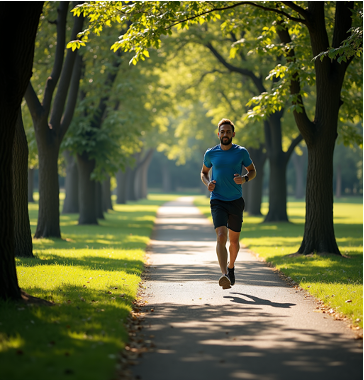
\includegraphics[width=\linewidth,  height=1.5cm]{figures/f1/1_1.png} &
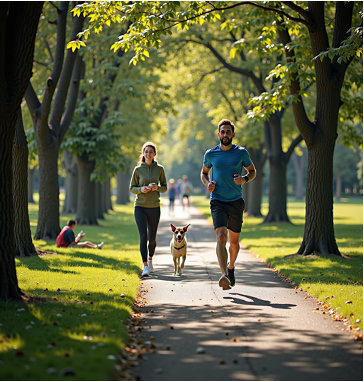
\includegraphics[width=\linewidth,  height=1.5cm]{figures/f1/1_2.png} &
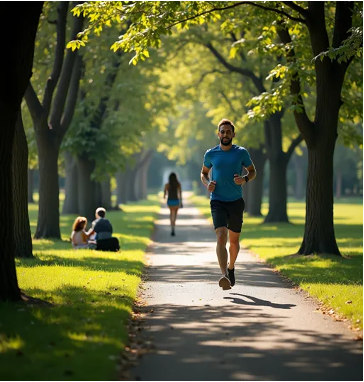
\includegraphics[width=\linewidth,  height=1.5cm]{figures/f1/1_3.png} &
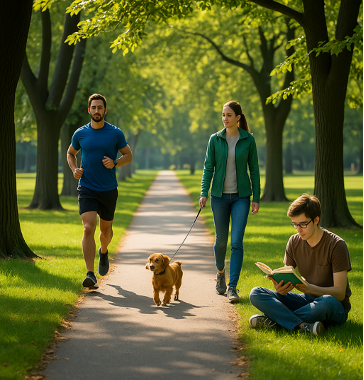
\includegraphics[width=\linewidth,  height=1.5cm]{figures/f1/1_4.png} &
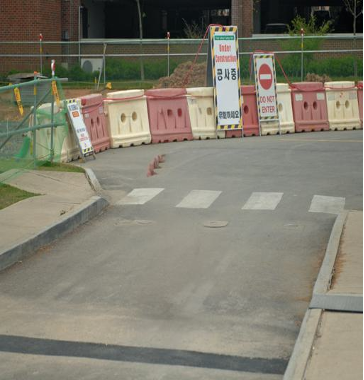
\includegraphics[width=\linewidth,  height=1.5cm]{figures/f1/4_1.png} &
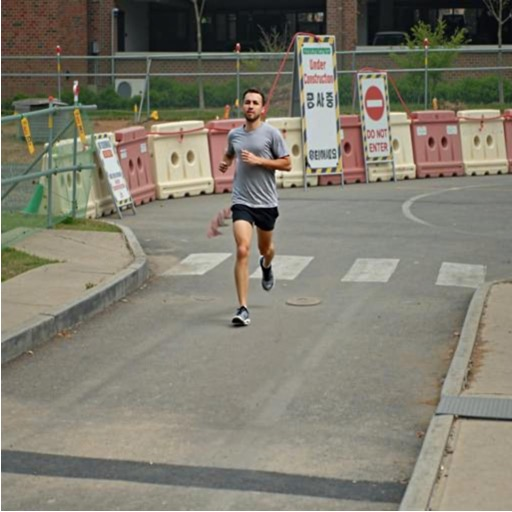
\includegraphics[width=\linewidth,  height=1.5cm]{figures/f1/4_2.jpg} &
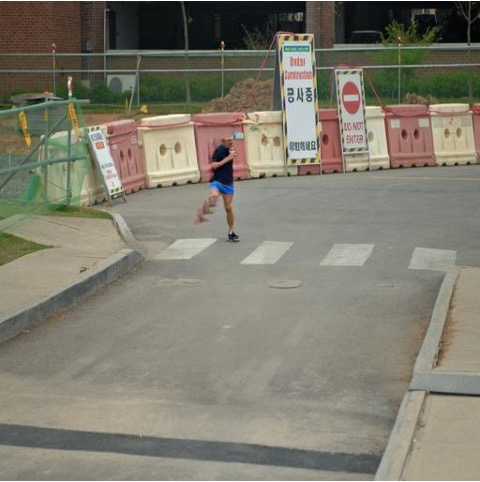
\includegraphics[width=\linewidth,  height=1.5cm]{figures/f1/4_3.jpg} &
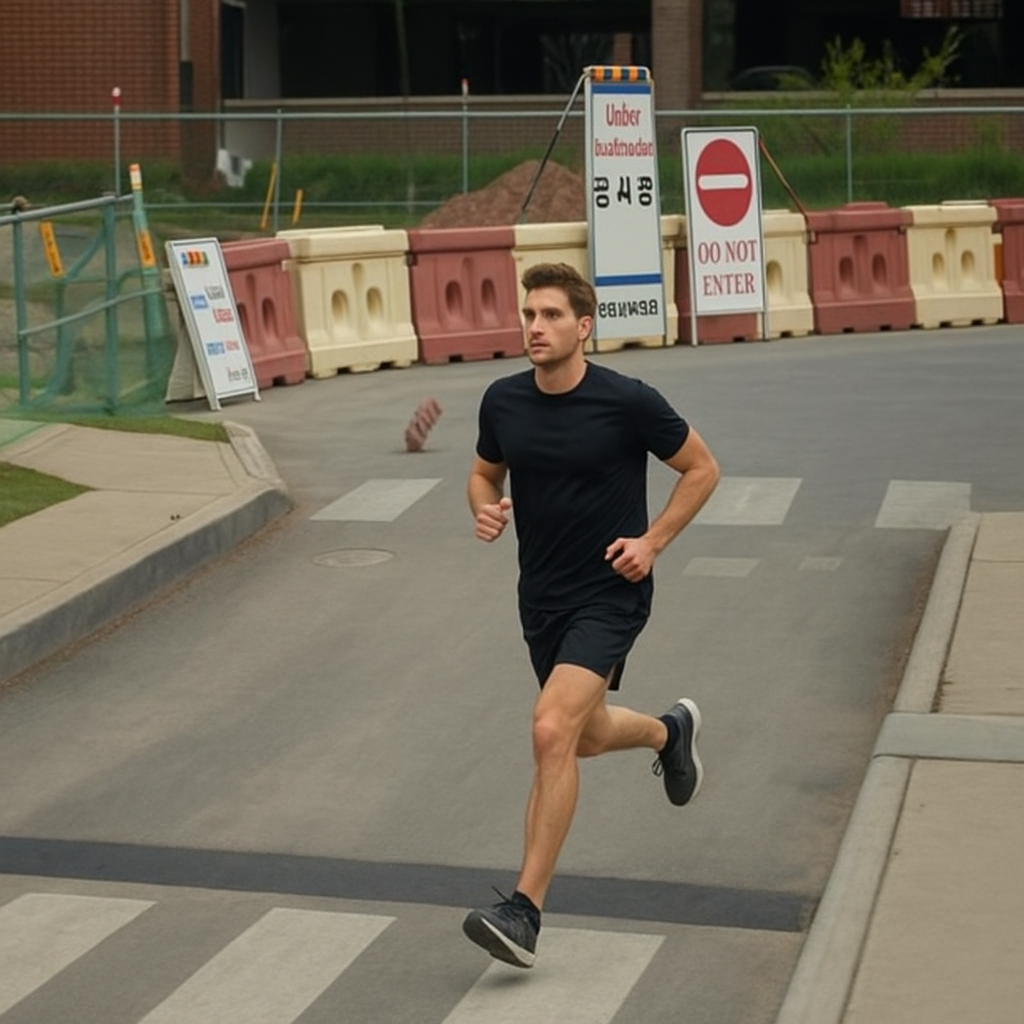
\includegraphics[width=\linewidth,  height=1.5cm]{figures/f1/4_4.png} \\[-1pt]

\multicolumn{4}{c}{\tiny (c) \textbf{Replace} the woman tennis player with a man tennis player.} & 
\multicolumn{4}{c}{\tiny (d) \textbf{Add} a baseball catcher on the field.} \\
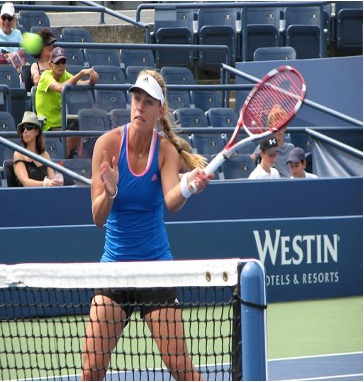
\includegraphics[width=\linewidth,  height=1.5cm]{figures/f1/2_1.jpg} &
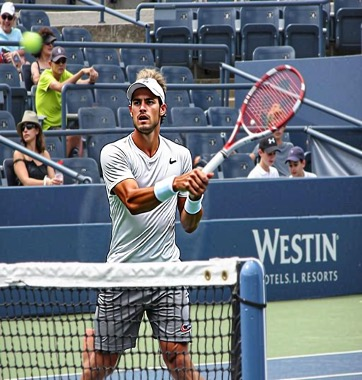
\includegraphics[width=\linewidth,  height=1.5cm]{figures/f1/2_2.jpg} &
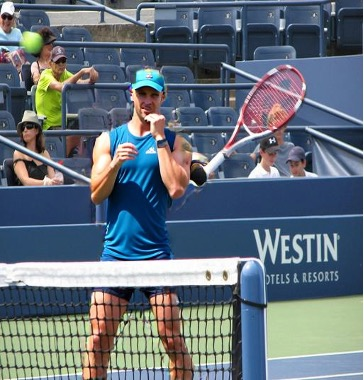
\includegraphics[width=\linewidth,  height=1.5cm]{figures/f1/2_3.jpg} &
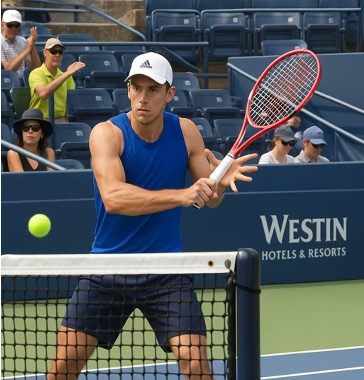
\includegraphics[width=\linewidth,  height=1.5cm]{figures/f1/2_4.jpg} &
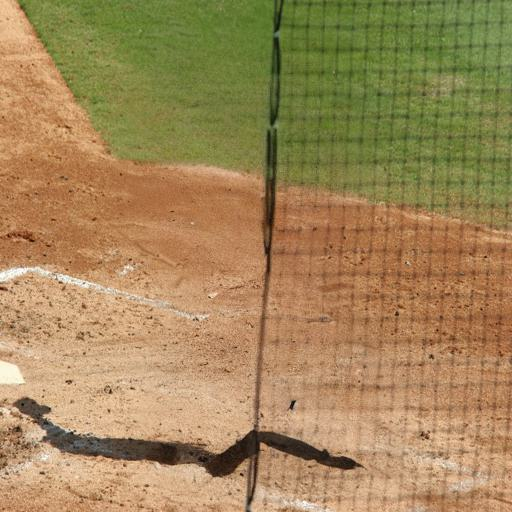
\includegraphics[width=\linewidth,  height=1.5cm]{figures/f1/5_1.jpeg} &
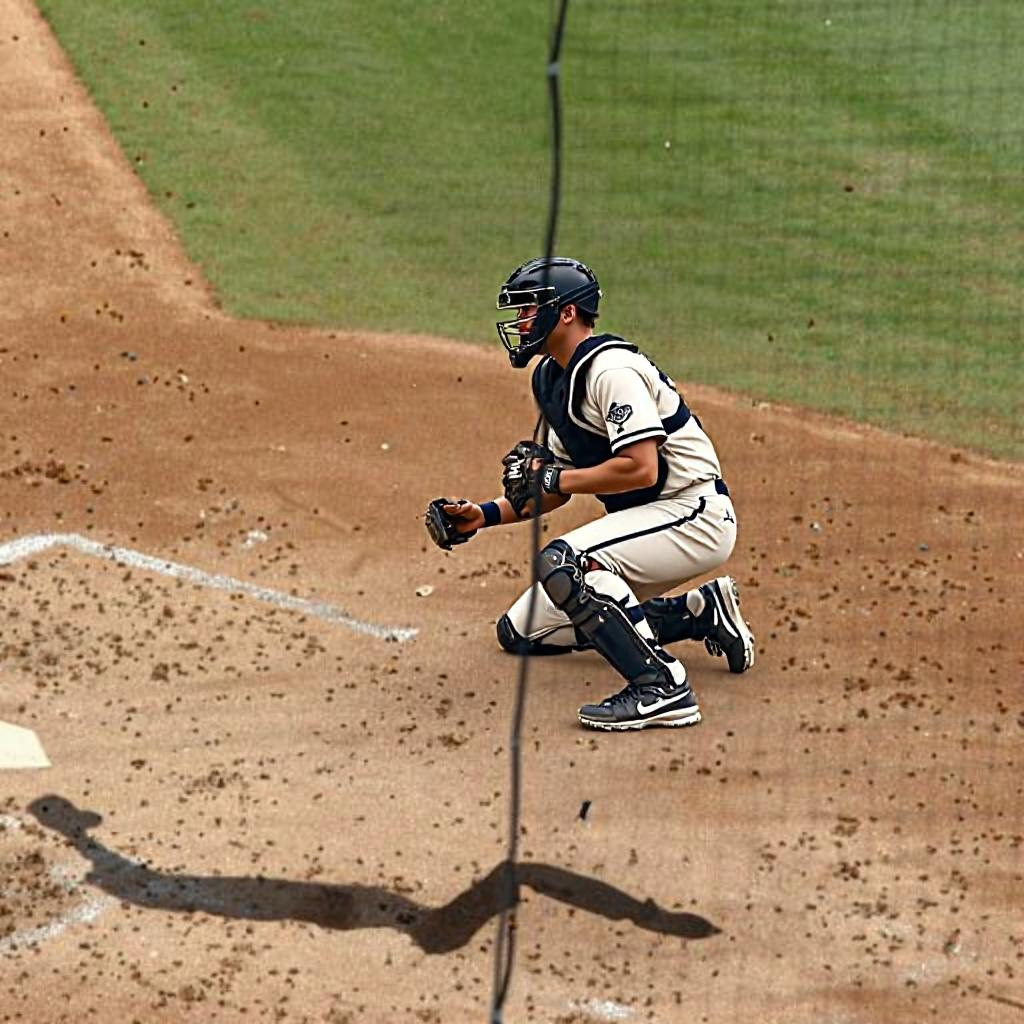
\includegraphics[width=\linewidth,  height=1.5cm]{figures/f1/5_2.jpeg} &
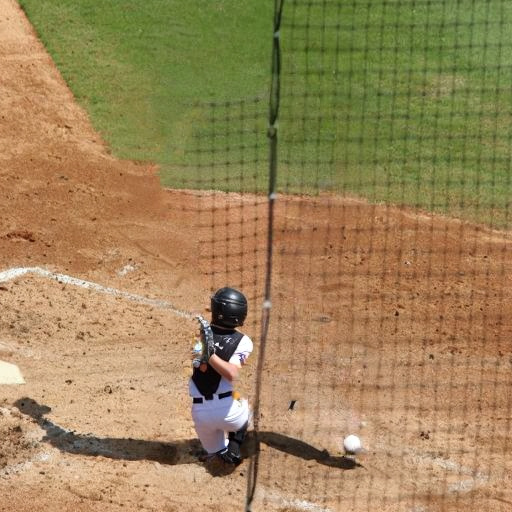
\includegraphics[width=\linewidth,  height=1.5cm]{figures/f1/5_3.jpeg} &
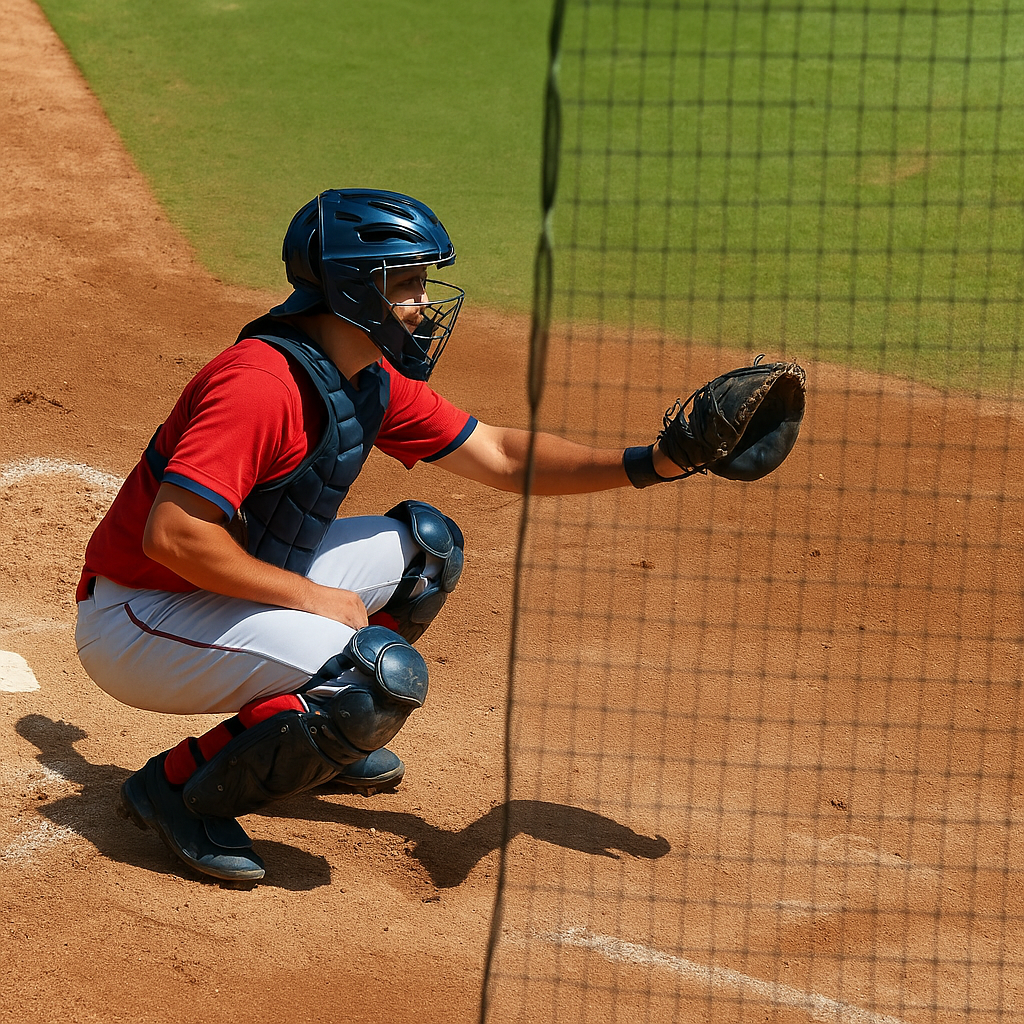
\includegraphics[width=\linewidth,  height=1.5cm]{figures/f1/5_4.png} \\[-1pt]

\multicolumn{4}{c}{\tiny (e) \textbf{Remove} the umbrellas.} &
\multicolumn{4}{c}{\tiny (f) \textbf{Replace} the pepper with three apples.} \\
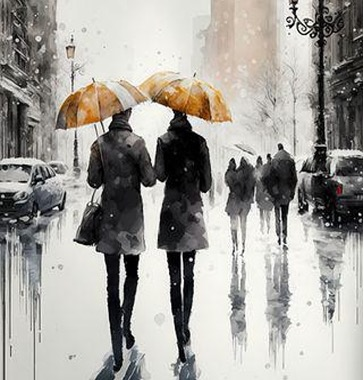
\includegraphics[width=\linewidth,  height=1.5cm]{figures/f1/3_1.jpg} &
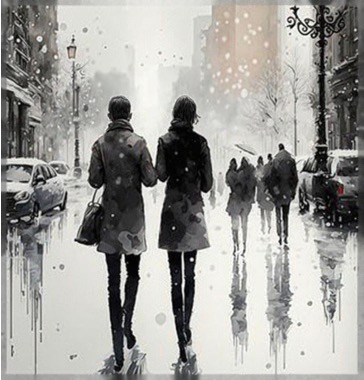
\includegraphics[width=\linewidth,  height=1.5cm]{figures/f1/3_2.jpg} &
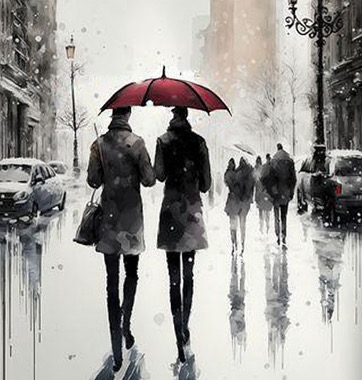
\includegraphics[width=\linewidth,  height=1.5cm]{figures/f1/3_3.jpg} &
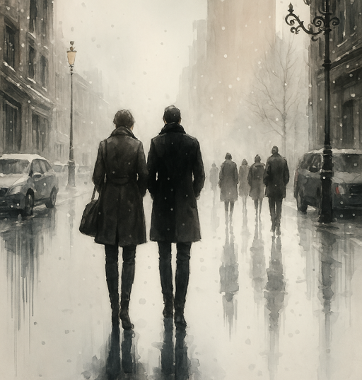
\includegraphics[width=\linewidth,  height=1.5cm]{figures/f1/3_4.png} &
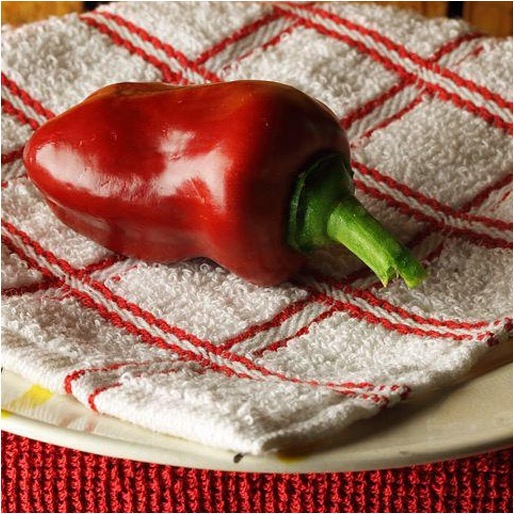
\includegraphics[width=\linewidth,  height=1.5cm]{figures/f1/6_1.jpg} &
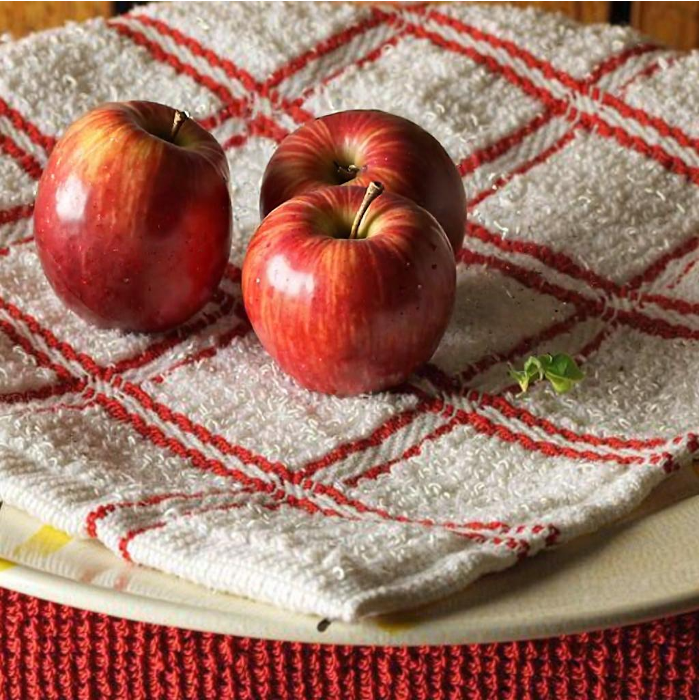
\includegraphics[width=\linewidth,  height=1.5cm]{figures/f1/6_2.png} &
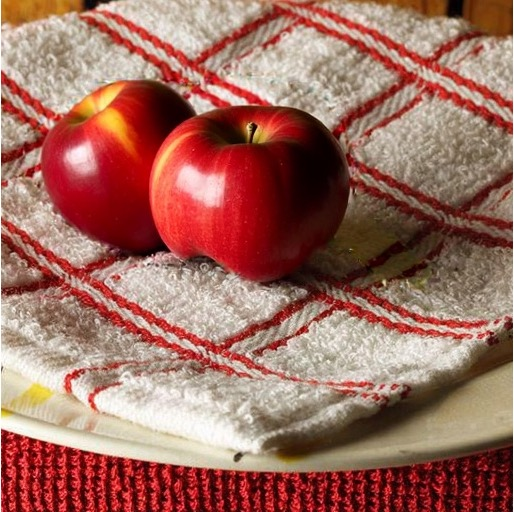
\includegraphics[width=\linewidth,  height=1.5cm]{figures/f1/6_3.jpg} &
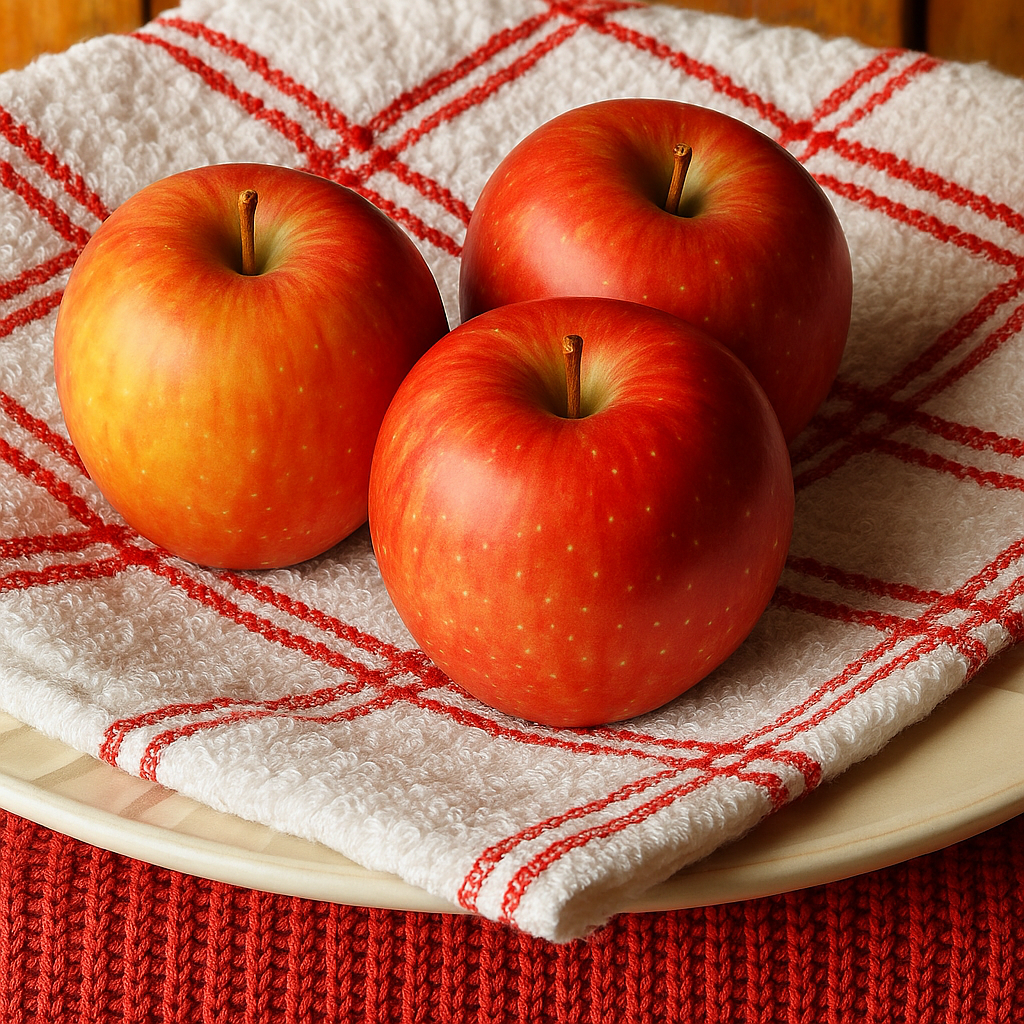
\includegraphics[width=\linewidth,  height=1.5cm]{figures/f1/6_4.png} \\
\multicolumn{1}{c}{{\scriptsize Input}} &\multicolumn{1}{c}{{\scriptsize CannyEdit}} &\multicolumn{1}{c}{{\scriptsize KV-Edit \citep{zhu2025kv}}}&\multicolumn{1}{c}{{\scriptsize GPT-4o \citep{OpenAI2025Introducing4O}}} &\multicolumn{1}{c}{{\scriptsize Input}} &\multicolumn{1}{c}{{\scriptsize CannyEdit}} &\multicolumn{1}{c}{{\scriptsize KV-Edit \citep{zhu2025kv}}}&\multicolumn{1}{c}{{\scriptsize GPT-4o \citep{OpenAI2025Introducing4O}}} \\
\end{tabular}
\caption{Examples of edits using our CannyEdit, KV-Edit~\citep{zhu2025kv}, and GPT-4o~\citep{OpenAI2025Introducing4O} (detailed text prompts and masks are omitted here; see Appendix~XX).}
\label{logo}
\end{figure}


% \begin{figure}[h!]
%     \centering
%     \includegraphics[width=0.9\linewidth]{figures/gpt2.png}
%     \caption{Examples of edits using CannyEdit, KV-Edit~\citep{zhu2025kv}, and GPT-4o~\citep{OpenAI2025Introducing4O} (detailed text prompts are omitted here; see Appendix~XX). The masks in (b) indicate the editing regions used by CannyEdit and KV-Edit. CannyEdit achieves strong text adherence, context preservation, and editing seamlessness, while KV-Edit struggles with instruction fidelity and editing seamlessness, and GPT-4o changes the image context excessively.}
%     \label{fig11}
% \end{figure}
% %
%\begin{figure}[t]
%    \centering
%    \includegraphics[width=0.99\linewidth]{figures/cat_example5.png}
%    \caption{Comparison of editing methods applied to the same example (a) of human subject insertion. The results of RFSolver-Edit \citep{wang2024taming}, (b.1–b.5), struggle to balance text adherence and context preservation. KV-Edit \citep{zhu2025kv}, using user-provided masks (c, d), enhances this balance but may introduce artifacts such as a {partially cropped subject} in (c.1), and {a partially generated extra cat} in (d.1). In contrast, our CannyEdit delivers seamless edits with robust text adherence and background consistency as shown in (c.2) and (d.2). With larger masks like in (d), our method refines the mask during generation to further improve context preservation, as demonstrated in (d.3).}
%    \label{fig1}
%\end{figure}
%
\section{Introduction}
\label{Sec:intro}
%

Recent advances in text-to-image (T2I) models have achieved substantial progress in quality and controllability \citep{rombach2022high,betker2023improving,chen2023pixart,esser2024scaling,blackforest2024FLUX}. These advancements have enabled diverse downstream applications, utilizing their enhanced quality, efficiency, and versatility. In this work, we address one of the most challenging applications: \emph{region-based image editing}, which entails modifying user-specified image areas (e.g., adding, replacing, or removing objects) while maintaining {overall image consistency}.
Region-based image editing extends standard T2I generation by introducing a critical constraint: the generated content must align not only with the text prompt {(\textbf{\textit{Text Adherence}})} but also with the existing visual context of the image {(\textbf{\textit{Context Fidelity}})}.{This problem is commonly known as the \textit{editability-fidelity trade-off}}.

% \textcolor{red}{(It seems \textit{context fidelity} is interchangeable with \textit{context preservation} in Fig. 2? May cause confusion.)}

%\kc{[``region-based'' seems more prevalent in the literature]} 

%Recent advances in text-to-image (T2I) models have demonstrated significant progress \citep{rombach2022high,betker2023improving,chen2023pixart,esser2024scaling,blackforest2024FLUX}. Building on these advancements, many downstream applications have emerged, leveraging the improved quality, efficiency, and versatility of these models.  In this paper, we focus on one of the most challenging applications: regional image editing. This task involves making specific edits (e.g., object adding, replacement or removal, see examples in Figure \ref{fig2}) to given areas of a generated or real-world image while keeping the rest of the image unchanged. It is effectively a conditioned T2I generation task, where the additional condition is the existing content in other parts of the image. 

%The key challenge is to ensure that the edits in the specific area not only match the input text but also blend coherently with the surrounding content. Ideally, if the editing is seamless, it should be difficult for viewers to discern the edited region or notice that the image has been modified by a model. 



A straightforward approach to region-based image editing involves collecting paired training data (before and after editing), along with corresponding text prompts, to train models for editing \citep{brooks2023instructpix2pix, zhang2023magicbrush, wasserman2024paint, li2024brushedit, hui2024hq, wei2024omniedit}. However, these methods often struggle to generalize beyond their training distribution--particularly in cases requiring realistic interactions, such as inserting people into complex scenes. This limitation is largely due to the lack of diverse, high-quality training data capturing such interactions.



% \sout{Consequently, by tapping into foundation T2I models’ ability to capture realistic object interactions from large-scale datasets, another line of research explores using these foundation models for regional editing in a training-free manner.}
To overcome this limitation, another line of research taps into the emergent capability of foundation T2I models to capture realistic object interactions learned from large-scale datasets.
The proposed methods are mostly designed to be training-free, hoping to fully preserve the robustness of the foundation models.
% \sout{While these methods were initially developed using UNet-based diffusion models \citep{hertz2022prompt, cao2023masactrl, tumanyan2023plug}, recent work has shifted to leveraging more advanced rectified-flow-based multi-modal diffusion transformers (MM-DiTs) \citep{rout2024semantic, wang2024taming, deng2024fireflow, tewel2025addit, zhu2025kv}.}
{These training-free approaches, initially developed upon UNet-based diffusion models~\citep{hertz2022prompt, cao2023masactrl, tumanyan2023plug}, has gradually shifted to leveraging more advanced rectified-flow-based multi-modal diffusion transformers (MM-DiTs)~\citep{rout2024semantic, wang2024taming, deng2024fireflow, tewel2025addit, zhu2025kv}.
A key advantage of MM-DiTs is that they offer a more flexible way to control the generation process, e.g., one can inject the query/key/value of source-image tokens (obtained via inversion \citep{deng2024fireflow,rout2024semantic,wang2024taming}) into that of the generated tokens at each denoising time step, improving context fidelity.}
{However, the improved context fidelity often comes at a cost of text adherence, as exemplified by results of RFSolver-Edit~\citep{wang2024taming} different injection steps in  Figure \ref{fig2} (b.1-b.5), where it struggles to strike a good balance between the two criteria. A quantitative study result on this is provided in Figure \ref{treadline}.}





% \sout{The newer DiT-based methods have demonstrated enhanced editing performance and greater flexibility compared to earlier approaches, leveraging the stronger generative capabilities of their base models. These methods primarily rely on injecting the source image's attention features (obtained via inversion~\citep{deng2024fireflow,rout2024semantic,wang2024taming}) into the generation of the edited image. While effective in certain cases, they face a critical challenge: balancing precise modifications to specific regions based on the target text prompt (\textbf{\textit{Text Adherence}}) while preserving the integrity of unedited areas (\textbf{\textit{Context Fidelity}}). This issue is termed the \textit{editability-fidelity trade-off}.}
% \sout{We show here that attaining an acceptable trade-off could be \textbf{infeasible} \kc{[``infeasible'' is a strong word]} for these methods, examplified by RFSolver-Edit \citep{wang2024taming}. Figure \ref{fig2} (a) presents quantitative results evaluating context fidelity and text adherence\footnote{Context fidelity is measured via cosine similarity of DINO embeddings \citep{caron2021emerging} between source and edited images. Text adherence is quantified as \( p_{\text{gdino}}(\textit{edited}) - p_{\text{gdino}}(\text{source}) \), where \( p_{\text{gdino}} \) denotes GroundingDINO's \citep{liu2024grounding} top-1 bounding box probability for the added subject.} for 15 editing examples of inserting a human subject into real-world images (Figure \ref{fig2}(b) provides a test example). The result shows that, under different attention injection steps of source image's features, RFSolver-Edit's outputs either adhere well to the text or preserve image context effectively, but no configuration achieves a strong balance. Visual examples of edits under different steps are shown in Figures \ref{fig2}(c.1–c.6).
% The root cause of this imbalance lies in the mixed visual information encoded in the source image's attention features. While injecting these features offers flexibility, it lacks precise control over what to \textcolor{orange}{be modified or preserved}.}

%We attribute the root cause of this inability to achieve a strong balance to the mixed nature of visual information encoded in the source image's attention features. While editing through the injection of such features offers flexibility, it falls short in providing precise control over which visual information should be modified and which should remain intact.

% \sout{To achieve a better trade-off, KV-Edit~\citep{zhu2025kv} introduces user-provided masks to separate edited and unedited regions during attention computation, updating features only in the edited region while preserving those of the unedited region from the source image. While improving the trade-off (orange points in Figure \ref{fig2}(a)), this approach can produce artifacts due to a disconnection between the background and edited regions, as seen in the partially cut subjects in Figure~\ref{fig2}(d.1) and the extra cat in Figure~\ref{fig2}(e.1).}

\begin{wrapfigure}{r}{0.5\textwidth}
  \vspace{-12pt} % Optional: to pull the figure up slightly
    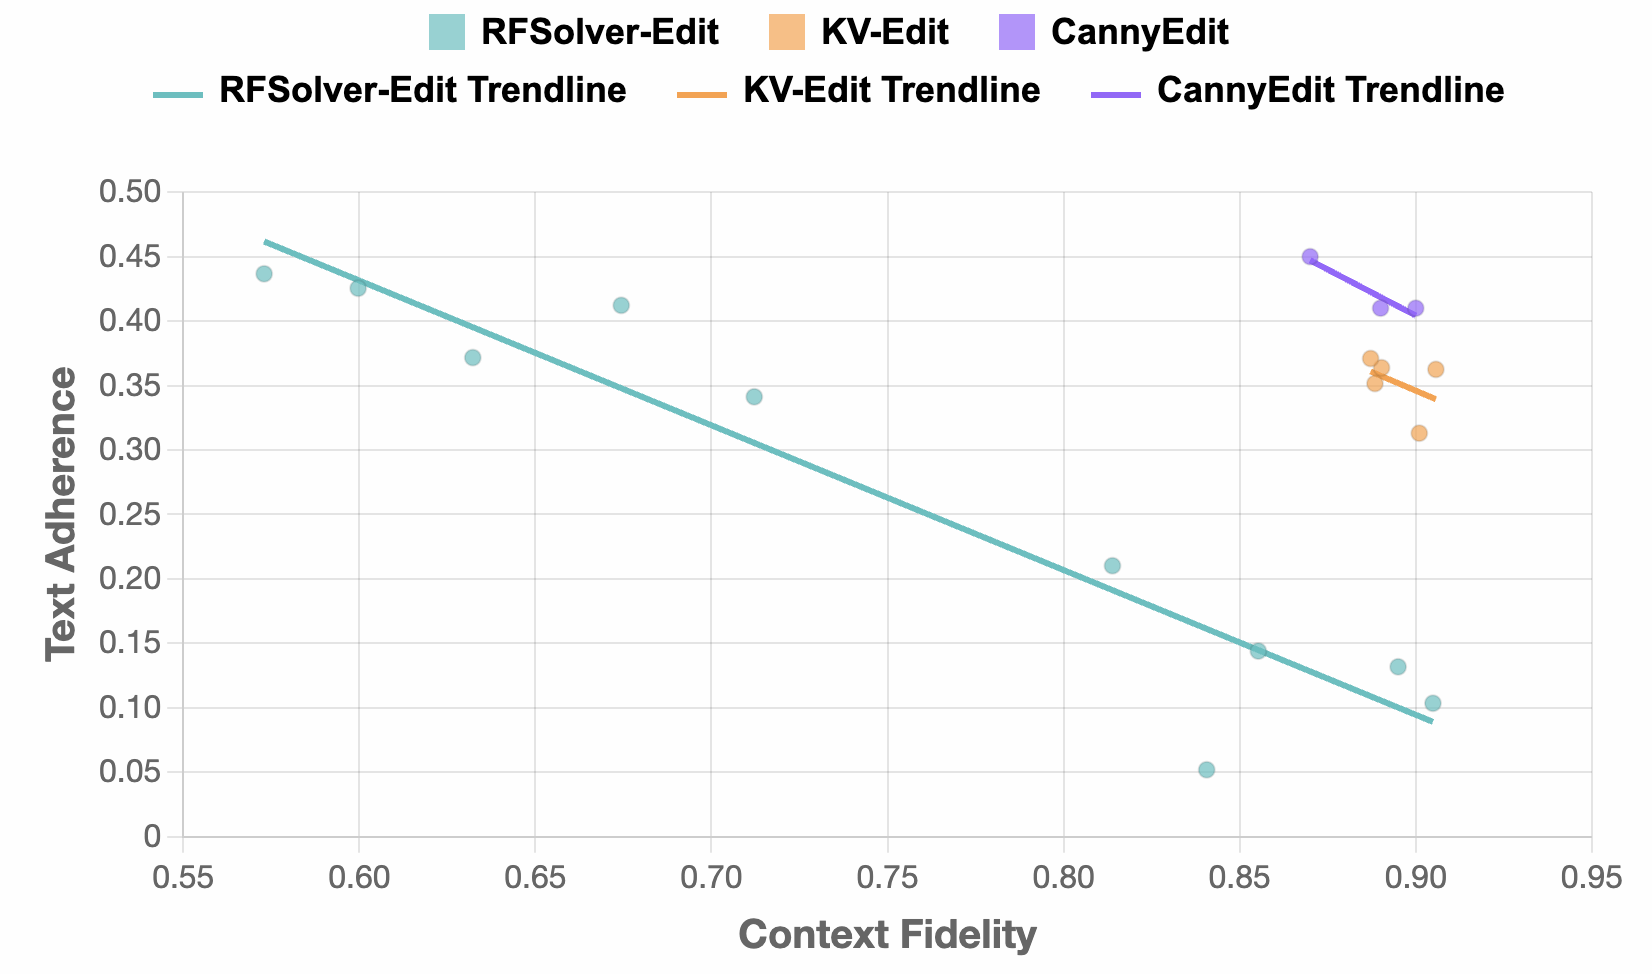
\includegraphics[width=1\linewidth]{figures/tl2.png}
\caption{\small Quantitative study of context fidelity and text adherence for RFSolver-Edit, KV-Edit, and CannyEdit on 15 human addition examples. Context fidelity is evaluated by cosine similarity of DINO \citep{caron2021emerging} embeddings between source and edited images, and text adherence is quantified via GroundingDINO~\citep{liu2024grounding}'s top-1 bounding-box confidence, defined as the confidence difference between edited and source images.  Different points for one method represent different hyperparameter settings.}
    \label{treadline}
      \vspace{-5pt} % Optional: reduce space below the figure
\end{wrapfigure}

To achieve a better trade-off, KV-Edit~\citep{zhu2025kv} introduces user-provided masks to separate regions to be edited from those to be preserved.
During generation, KV-Edit only updates the image tokens in the unmasked regions while keeping the masked regions intact.
Although this greatly improves the trade-off (as shown by the orange points in Figure~\ref{treadline}, KV-Edit sometimes produces conspicuous artifacts and inconsistencies at the mask boundary, especially when the mask is not precise.
Typical examples are shown in Figure~\ref{logo} (b, d) and Figure~\ref{fig2} (c.1, d.1).
% This creates a burden on the users, potentially impacting their experience.
The imperfection highlights another key quality aspect of region-based image editing: \textbf{\textit{Editing Seamlessness}}, which is essential to good user experience.
{We hypothesize that the boundary artifacts of KV-Edit originate from its hard context replacement strategy, which ensures context fidelity but breaks the interdependency necessary for smooth boundary transitions.}




   % 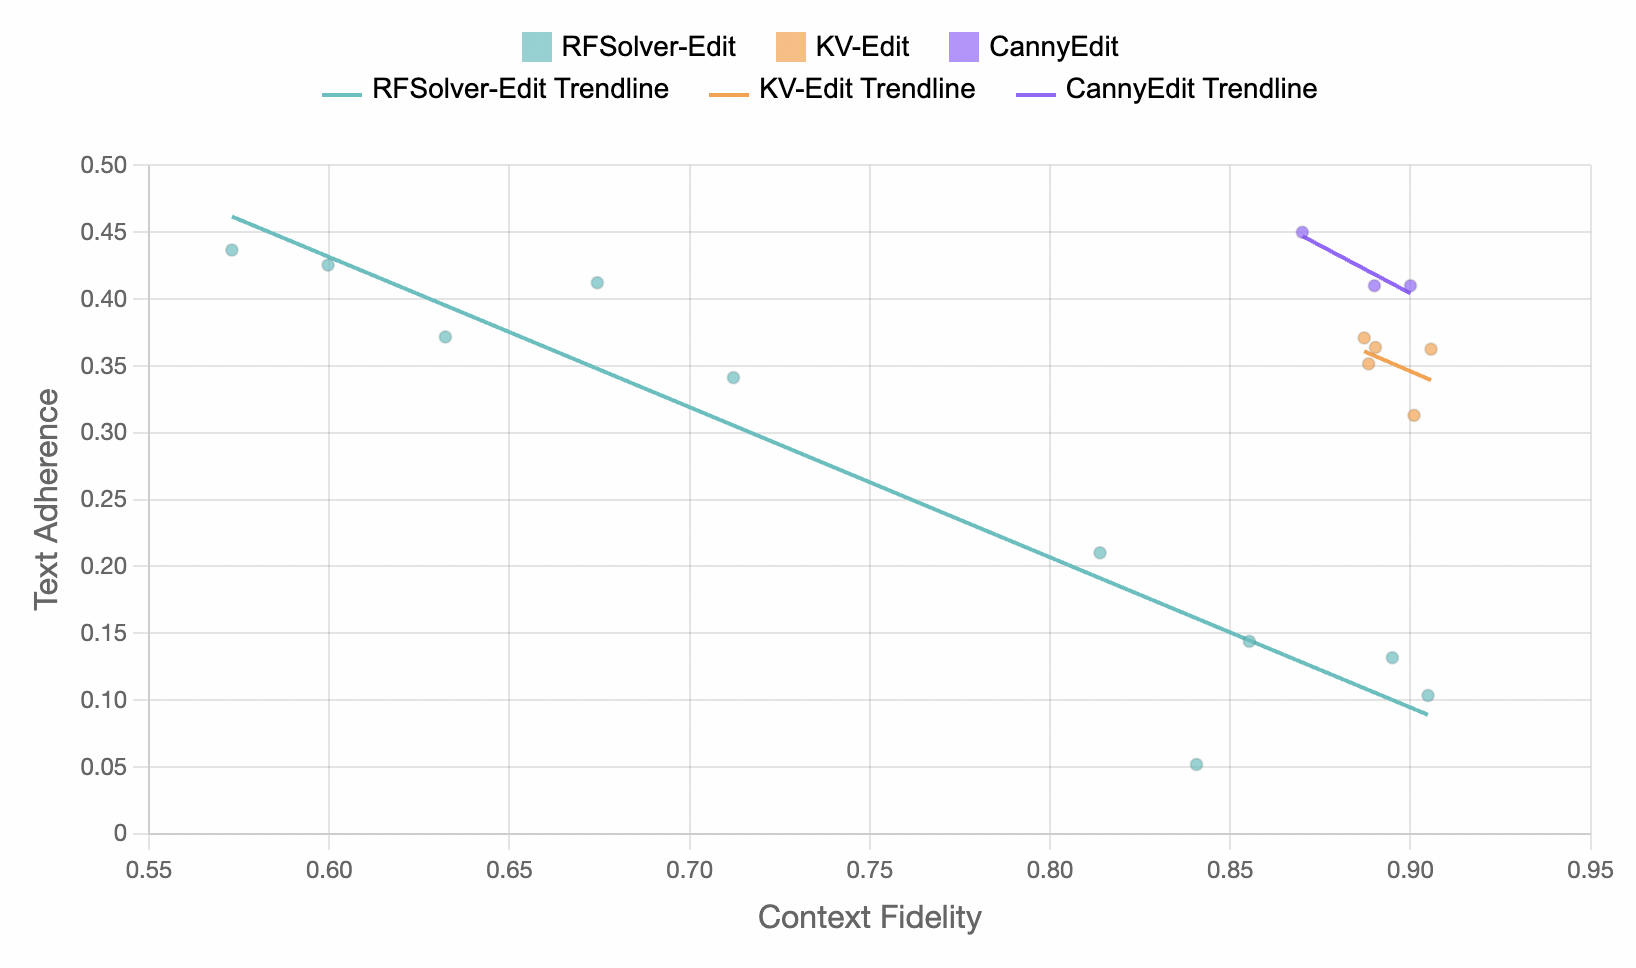
\includegraphics[width=0.7\linewidth]{figures/trendline.png}
   %  (a)
   % \caption{Quantitative comparison of context fidelity (cosine similarity of DINO \citep{caron2021emerging} embeddings between source and target images) and text adherence (quantified as \( p_{\text{gdino}}(\textit{edited}) - p_{\text{gdino}}(\text{source}) \), where \( p_{\text{gdino}} \) is GroundingDINO's \citep{liu2024grounding} top-1 bounding box probability for the added subject) for RFSolver-Edit, KV-Edit, and our CannyEdit, evaluated on 15 examples of adding human subjects. Different points for one method represent different hyperparameter settings}



%(RFSolver-Edit: attention injection steps; KV-Edit: skip steps, reinitialization).

%Achieving all three simultaneously is inherently challenging because the objectives often conflict. For instance, leaving an image untouched yields perfect contextual fidelity but offers no adherence to the given target text prompt. Conversely, forcing the background region to remain identical to its original appearance may safeguard fidelity, yet it can impair seamlessness—e.g., removing a person while leaving the cast shadow makes the edit conspicuous.


%A small-scale study involving the 20 images of human insertion edited by KV-Edit, mixed with original images, was presented to 100 first-year undergraduate students without a technical background in T2I generation.\footnote{Note that participants were not shown both the source image and its edited counterpart simultaneously in one run of the study.} The participants were asked to judge if each image was AI-edited. The study revealed that KV-Edit produced images with noticeably low editing seamlessness, as the rate of participants identifying the images as AI-edited (xxx\%) was significantly high compared to a baseline rate for the unedited images (xxx\%).


% Canny-\underline{Rx}: Selective Canny Control and \underline{R}egional Te\underline{x}t Guidance for Training-free Image {E}diting


%for the text adherence and seamless editing

%Our key innovation lies in selective masking: by masking ControlNet’s outputs in user-specified editable regions before their addition to the T2I model, we relax structural constraints in regions where edits occur (thereby enabling text-guided edits) while strictly preserving the original layouts elsewhere.  To further enhance context fidelity, we also incorporate the Canny ControlNet during the inversion of the source image. The ControlNet's outputs that are masked and added into the generation of the edited image are obtained from this inversion process.

 %Our method emphasizes the importance of applying regional text guidance at different levels for effective and seamless editing:


%================================================================

% Building on the challenges faced by attention-based methods and inspired by KV-Edit’s use of user-provided masks for improved balance, we propose a novel training-free editing method to achieve a better trade-off between editability and context fidelity. To avoid unnatural results caused by disconnected attention computations, our approach retains the core attention mechanisms while introducing a key innovation: the selective use of Canny ControlNet’s outputs \citep{zhang2023adding} for image editing.




\kcc{Building upon these insights, we propose a novel training-free image editing method, \emph{CannyEdit}, that achieves the state of the art in editability-fidelity trade-off, in addition to a significant qualitative improvement in seamlessness as validated by comprehensive user studies.
Specifically, our approach involves three key innovations.
First, we \textcolor{red}{selectively use} \emph{Canny ControlNet's outputs}~\citep{zhang2023adding} to relax the structural constraints in the desired edit region while preserving the original image layout elsewhere.
Second, we propose a dual-prompt strategy that uses a \emph{local prompt} to provide fine guidance to edited regions along with a global \emph{target prompt} to ensure coherence between the edited regions and the context.
Last but not least, we adopt soft masking at the boundary region of the user-specified mask to enable smooth and seamless transitions across regions in complex scenes. \textcolor{red}{[We don't use forceful attention injection like previous methods. Instead, we only change the input conditions and the attention masks to achieve natural edits.]}}

% Canny edge maps \citep{canny1986computational} extract structural information from images by detecting edges, effectively capturing key layout details. Canny ControlNet, a plug-and-play module for foundation T2I models, processes these input edge maps using copied denoising block structures, injecting layout guidance by adding its outputs to corresponding blocks in the base T2I model. Our method proposes to integrate Canny ControlNet with a selective masking strategy. Specifically, masking features corresponding to edited regions in the ControlNet's output relaxes structural constraints in user-defined editable areas (enabling text-guided edits) while preserving the original layout elsewhere. \textcolor{orange}{To ensure smooth transitions between the edited and background regions, in addition to masking the Canny control on the edit region, we also relax the control strength on the boundary region by lowering the control strength parameter.}
\begin{figure}[t]

    \centering
    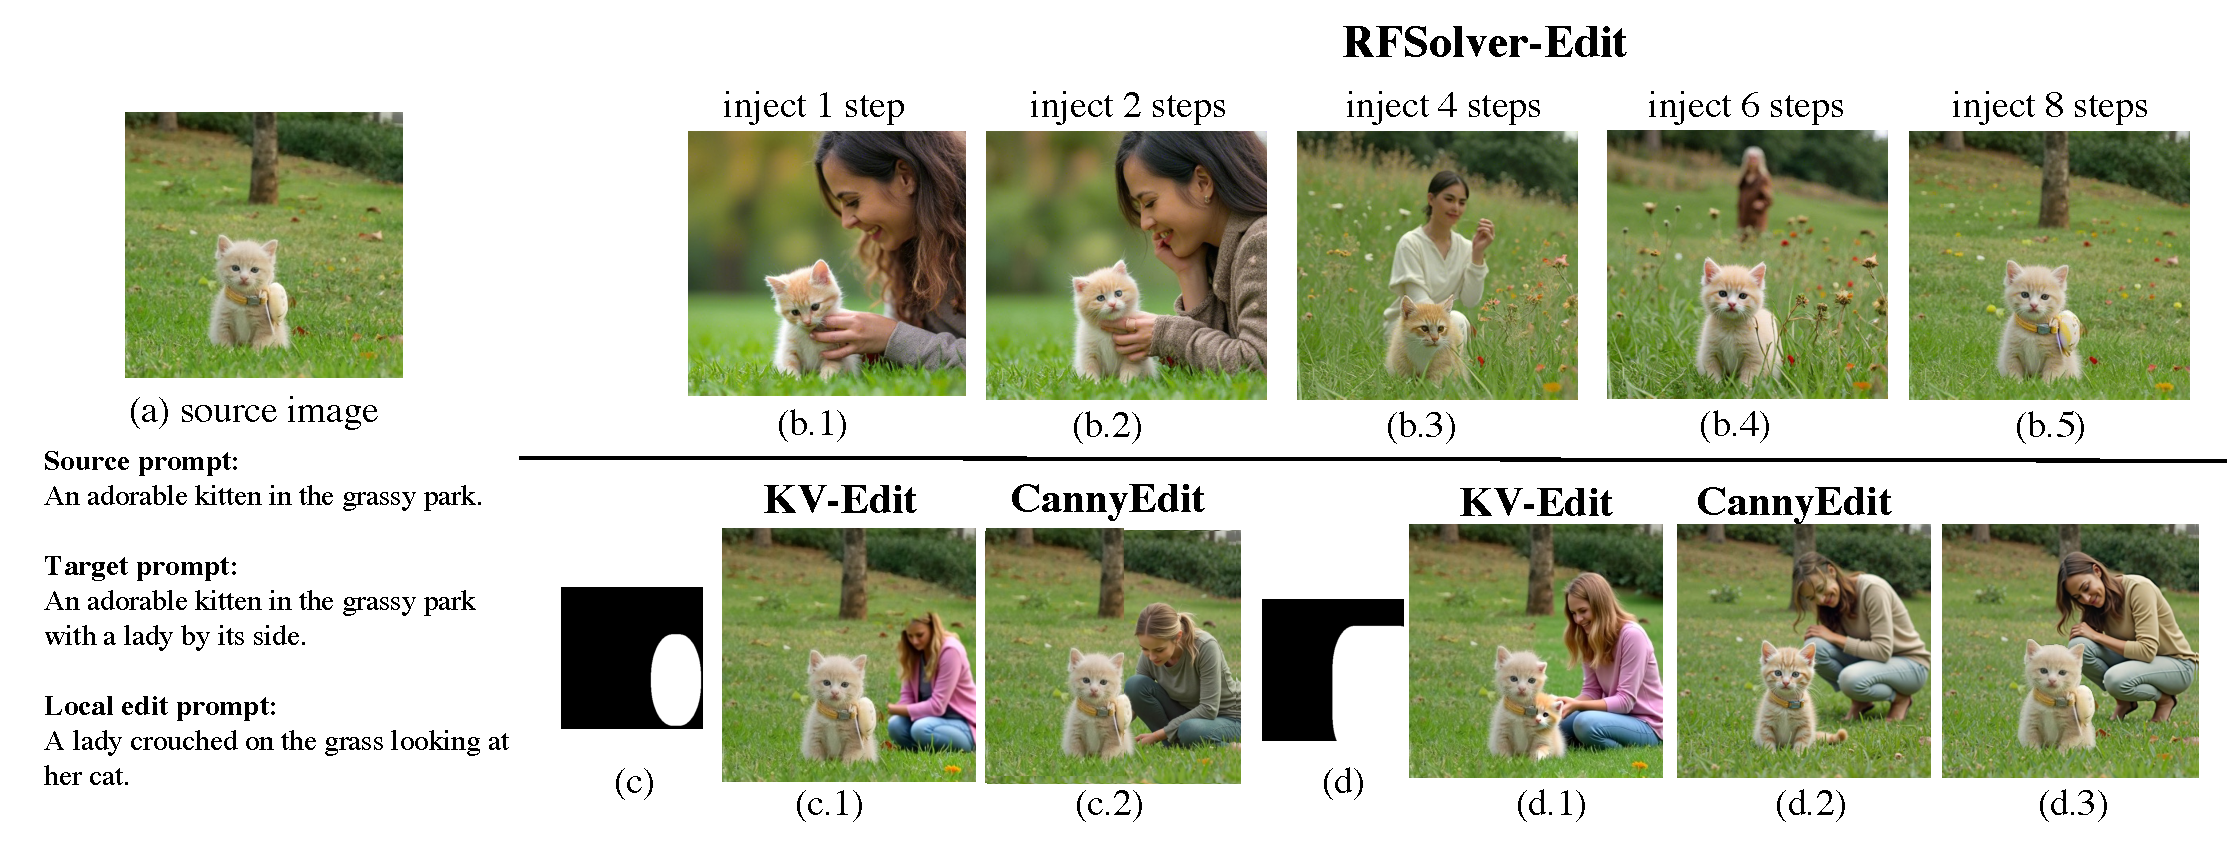
\includegraphics[width=0.9\linewidth]{figures/cat3.pdf}
      \caption{Editing results of different methods: RFSolver-Edit's outputs fail to balance context fidelity and successful addition simultaneously. While KV-Edit and CannyEdit deliver a better trade-off, CannyEdit results in the more natural and seamless editings while KV-Edit's results introduce artifacts such as a {partially cropped subject} in (c.1), and {a partially generated extra cat} in (d.1).}
  %  \caption{(a) Quantitative Comparison of context preservation and text adherence for RFSolver-Edit, KV-Edit, and our proposed CannyEdit, evaluated on 15 examples of adding human subjects. Different points for one method represent different hyperparameter settings. RFSolver-Edit struggles to balance context preservation and text adherence effectively, while KV-Edit achieves a notably improved trade-off. Our CannyEdit method further improves this trade-off, significantly increasing text adherence while maintaining comparable context preservation (the largest point for CannyEdit represents our default setting, and the other two points are created by applying additional blending with the source image on the background regions). (b-e) shows visual examples of different methods: apart from the context preservation and text adherence, we can see that our CannyEdit results in the more natural and seamless editings while KV-Edit's results introduce artifacts such as a {partially cropped subject} in (d.1), and {a partially generated extra cat} in (e.1). }
  % \caption{(a) Quantitative comparison of context fidelity vs. text adherence for RFSolver-Edit, KV-Edit, and our CannyEdit on 15 human addition tasks. RFSolver-Edit shows poor balance, KV-Edit improves the trade-off, and CannyEdit achieves the best results—boosting text adherence while preserving context. Different points for one method represent different hyperparameter settings. Largest CannyEdit point denotes default setting; smaller points reflect applying additional cyclical blending with the source image on the background regions in a higher frequency. (b–e) Visual examples: RFSolver-Edit's outputs fail to balance context fidelity and successful addition simultaneously. While KV-Edit and CannyEdit deliver a better trade-off, CannyEdit results in the more natural and seamless editings while KV-Edit's results introduce artifacts such as a {partially cropped subject} in (d.1), and {a partially generated extra cat} in (e.1).}
    \label{fig2}
\end{figure}

%As ControlNet’s outputs are optional for T2I models, this approach does not interfere with their core attention computations.

% With selective masking removing structural constraints in editable regions, textual guidance becomes critical for directing edits. To address this, we propose a dual-prompt strategy: \emph{local prompts} confine edits to user-specified regions, ensuring precise object generation, while a \emph{target prompt}, describing the global image context after editing, ensures coherence between edited areas and their surroundings. Figure~\ref{fig2} illustrates an example of local and target prompts, both of which are essential for high-quality editing. Following prior work \citep{chen2024training}, we implement text control via attention masks, enforcing spatial constraints in a training-free manner. \textcolor{orange}{Departing from the typical attention mask in \citep{chen2024training}, we additionally allow the boundary region to attend to both the edited and background regions to achieve a smooth transition. Further adjustments to the form of attention masks to enhance their applicability across various editing tasks will be detailed in the method section. }


In summary, we make the following key contributions in this paper:

\vspace{-1mm}
\begin{itemize}[leftmargin=5mm]
\item We propose CannyEdit, a novel region-based image editing method leveraging foundation T2I models and their Canny ControlNet components in a training-free manner. By introducing selective Canny control and soft boundary masking, CannyEdit enables high-quality region-based edits that seamlessly blend in with the context. Combined with dual-prompt guidance, CannyEdit achieves text-adherent, context-aware edits with a strong editability-fidelity balance.
% \textcolor{orange}{Our special treatments on the mask boundary further ensures seamless integration between edited and unedited regions.}

\vspace{-1mm}

\item CannyEdit serves as a flexible and versatile editing framework applicable to various regional image editing tasks, including insertion, replacement, removal, object transfer, and context modifications.
\kc{In principle, our framework can also be easily extended to incorporate other forms of control unit such as IP-Adapter~\cite{}, ....}

\vspace{-1mm}

\item CannyEdit outperforms strong training-free baselines like KV-Edit~\citep{zhu2025kv}, with 2.93\%, 5.35\%, and 10.49\% improvements in terms of editability-fidelity trade-off on object replacement, addition, and removal on real-world images. It also surpasses open-source training-based methods such as BrushEdit \citep{li2024brushedit} and PowerPaint \citep{zhuang2023task}. User study results demonstrate that CannyEdit's results are more natural with a significant lower likelihood to be identified as AI-edited.  %In a user study on editing seamlessness, only 49.20\% of the general public and 42.00\% of AIGC experts identified CannyEdit's outputs as AI-edited when the edited results were paired with unedited real-world images. This is much lower compared to 76.08\% and 82.00\% for the next best method. This shows that our edits are more natural and less detectable.

\end{itemize}

%The ControlNet outputs, masked and added during generation, are derived from the source image's inversion to enhance context fidelity.

% Witnessing the challenge in the attention-based methods and following the way in KV-Edit to apply an user-given mask for a bettering balance maintenance, we propose a novel training-free  editing method to allow a better balance between editability and context fidelity. To avoid the unnatural results cased by the disconnected attention computation, we instead seek a way without altering the core attention mechanisms. The key innovation of our method lies on the selective use of Canny ControlNet's outputs \cite{zhang2023adding} for image editing. Canny ControlNet is a plug-and-play module for foundation T2I models, employing copied denoising blocks’ structures to process input edge maps. It injects layout guidance by adding its outputs to corresponding blocks in the base T2I model. To maintain a good balance on the editability-fidelity trade-off By integrating Canny ControlNet \citep{zhang2023adding} with a selective masking strategy, we relax structural constraints in user-specified editable regions (enabling text-guided edits) while strictly preserving original layouts elsewhere. The ControlNet’s outputs, masked and added during generation, are derived from the inversion of the source image to enhance context fidelity. 

% Witnessing the imperfections of previous methods, in this work, We introduce \textbf{\textit{CannyEdit}}—a training-free pipeline for image editing based on pretrained diffusion models and their Canny ControlNet components \citep{zhang2023adding}. The method is designed to reconcile the three competing goals of {text adherence}, {context fidelity}, and {editing seamlessness}. 

% CannyEdit relies on two complementary mechanisms: (1) \textbf{Selective Canny control}.  Canny ControlNet \citep{zhang2023adding} is a plug-and-play module for foundation T2I models, employing mirrored denoising blocks’ structures to process input edge maps. It injects layout guidance by adding its outputs to corresponding blocks in the base T2I model. By integrating Canny ControlNet \citep{zhang2023adding} with a selective masking strategy, we relax structural constraints in user-specified editable regions (enabling text-guided edits) while strictly preserving original layouts elsewhere. The ControlNet’s outputs, masked and added during generation, are derived from the inversion of the source image to enhance context fidelity. (2) \textbf{Dual-Prompt Guidance}. As selective masking eliminates structural constraints in editable regions, textual guidance becomes critical for directing edits. For this,  we propose a dual-prompt strategy: \emph{local prompts} are confined to user-specified edit regions, ensuring the desired objects are generated precisely within the specific areas, while a \emph{target prompt}, describing the global image context after editing, applies to the entire image, maintaining coherent interactions between edited region and other image contexts. Figure \ref{fig2}(a) shows an example of local and target prompts. We will show that both prompts are important in editing.  Following prior work \citep{chen2024training}, the text control is implemented via attention masks to enforce spatial constraints in a training-free manner.




% 

% \vspace{-1mm}
% \begin{itemize}
% \item Divergent from previous training-free methods that rely on attention features to maintain source image information. In this work, we propose another possibility, to preserve the image context via source image's ControlNet information and propose selective Canny control to allow editabiity on the speciifc image region. Combined with regional text guidance that provides precise text control for the edit region, our approach can achieve more seamless edits without  requiring retraining;
% %altering the T2I model’s core attention mechanisms or
% \item The proposed CannyEdit serves as an editing framework, can flexibly apply to different regional image editing tasks, including adding, replacement, removal, object transfer (replacement with shape exactly unchanged) context change and so on. As it does not altering the T2I model’s core attention mechanisms, it has potentials to combine with other modules like IP-Adapter, Pose ControlNet and so on to support more tasks;
% \item Performance. Compared to the training-free editing methods that maintain the editability-fidelity trade-off best, KV-edit, our method enjoy 2.75\%, 5.11\% 10.49\%  improvement on the trade-off score in terms of replacement, adding and remvoal on the real-world image editing involving complex interaction with context. Also, our method beat the open-souce training-based methods (like BrushEdit \citep{li2024brushedit}, Powerpaint\\citep{zhuang2023task}). In terms of editing seamlessness, we conduct an user study. when paired with our editing results with the real-world images, we ask which image is more likely to be AI-edited, the users hardly random pick the previous while users pick results of other methods as AI-edited easily. The pick rate as AI-edited on our method for general public and AIGC expert users is 49.2\% and 42.0\% respectively while the second-best number achieved on evaluated previous open-source methods are 76.08\% and 82.0\% respectively. 


% \end{itemize}

% tasks, performance



% In summary, we make the following key contributions in this paper:
% \vspace{-1mm}
% \begin{itemize}
%     %\item To the best of our knowledge, our proposed CannyEdit is the first Canny-guided regional image editing method, incorporating the selective Canny control to enable both the local editability and background fidelity;
%     \item To the best of our knowledge,  our proposed CannyEdit CannyEdit is the first Canny-guided regional image editing framework built on foundation T2I models. We introduce a selective Canny masking mechanism that flexibly suppresses edge guidance in user-specified regions, enabling precise local edits while preserving the structural layout. %and background fidelity of unedited areas through image inversion with integrated Canny ControlNet signals.
%     \item CannyEdit is highly flexible, being able to apply different regional image editing tasks, including object transfer, adding, replacement, removal; context change and object personalization;
%     \item We show that CannyEdit maintains high level of image quality, background preservation and text alignment on the PIE-Bench \citep{brooks2023instructpix2pix}. Since there is lack of benchmark that evaluates the editing seamlessness performance in real-world image editing, we construct a ``real-world editing seamlessness'' benchmark and conduct user study to evaluate if the users can discern the edited region or notice that the image has been modified by a model. CannyEdit shows significantly improved seamlessness compared to previous training-based and training-free methods \textcolor{red}{[Need exact numbers]}. 
% \end{itemize}








% \begin{figure}[t]
%     \centering
%     \includegraphics[width=0.5\linewidth]{image2.png}
%     \caption{Group Space-Progress2504-paperfigures-figure2_v0428.png.}
%     \label{fig2}
% \end{figure}



\section{Related work}
\subsection{Training-based image editing methods}


A significant number of studies focus on training-based methods for image editing, which rely on synthetic data generated via large language models and T2I models \citep{brooks2023instructpix2pix, hui2024hq}. While beneficial for teaching models to follow instructions, these methods may not capture all real-world nuances, potentially limiting performance on complex edits. Alternatively, some works collect real-world images and manually annotate data or use task specialists to generate target images \citep{zhang2023magicbrush, wasserman2024paint, wei2024omniedit}. However, scaling these datasets is challenging, and both dataset construction and model training incur considerable computational costs.

The challenge of dataset scalability limits the generalization performance of training-based methods. We argue that training-free methods could be viable alternatives, as they are computationally efficient and preserve the generated image quality of the foundation T2I model, reducing the risk of overfitting or degradation in image quality.



% A significant number of studies focus on training-based methods for image editing. Although it is beneficial to teach model to learn to follow instructions, it is very expensive to collect high-quality image editing data. Therefore, many works propose to use synthetic data. For example, InstructPix2Pix \citep{brooks2023instructpix2pix} uses a language model (GPT-3 \citep{brown2020language}) and a T2I model (Stable Diffusion \citep{rombach2022high}) to generate a synthetic dataset of image editing examples. Similarly, HQ-Edit \citep{hui2024hq} uses GPT-4V \citep{openai2023gpt4v} and DALL-E 3 \citep{ramesh2021zero}. These methods, which reply on synthetic data, may not capture all real-world nuances, potentially limiting performance on complex edits.

% A different line of work collects real-world images and invites humans to manually annotate data or use task specialists (pre-trained image-editing models) to generate target images. MagicBrush \citep{zhang2023magicbrush} features 10K manually annotated image editing triplets (source image, instruction, target image), yet scaling this dataset is challenging. PIPE (Paint by Inpaint Edit) \citep{wasserman2024paint} comprises around 1 million pairs, focusing exclusively on object addition tasks using an inpainting model. OmniEdit \citep{wei2024omniedit}, a generalist model, is trained on over 1 million diverse pairs, utilizing feedback from seven specialist models. However, both dataset construction and model training incur considerable computational costs, which escalate with the models' complexity and the volume of data processed.

% The challenge of dataset scalability limits the generalization performance of training-based methods. We argue that training-free methods could be viable alternatives—not only because they are computationally efficient, but also because they preserve the image quality of the original T2I model, reducing risk of overfitting or degradation on image quality.

%MagicBrush \citep{zhang2023magicbrush} consists of 10K manually annotated real image editing triplets (source image, instruction, target image), but it is very difficult to scale it up.  PIPE (Paint by Inpaint Edit) \citep{wasserman2024paint} contains approximately 1 million image pairs, where objects are removed from source images using an inpainting model, but it is only focused on object adding task. OmniEdit \citep{wei2024omniedit} is a generalist model trained on over 1 million pairs covering diverse editing skills, leveraging the supervision from seven specialist models. The computational costs of constructing the datasets and training the model are significant, as they scale with the complexity of the models and the volume of data being processed. 



\vspace{-2mm}

\subsection{Training-free image editing methods}

%Existing training-free methods typically follow a two-stage attention-based editing pipeline: (1) Inversion: the source image is inverted into the DiT’s latent space to extract attention features at each denoising step; (2) Source-attention injection: these features are injected into the attention computation during the generation of the target image.

% For training-free methods, it is crucial to select a strong text-to-image model as foundation. The modern text-to-image models change from diffusion-based UNet models (e.g., Stable Diffusion 1.5 \citep{rombach2022high}) to rectified-flow-based transformer models (e.g., FLUX.1-dev \citep{blackforest2024FLUX}). Prompt-to-Prompt \citep{hertz2022prompt} and MasaCtrl \citep{cao2023masactrl} are  two of the early works which manipulated the cross-attention maps in the UNet model between text tokens and image regions. Attention manipulation, particularly cross-attention or self-attention, becomes a common practice in many training-free image editing methods\citep{rout2024semantic,deng2024fireflow,tewel2025addit,zhu2025kv}.

% Inversion is another important strategy to improve the integrity of unedited regions. Methods like RFSolver-Edit \citep{wang2024taming} and FireFlow \citep{deng2024fireflow} enhance inversion precision for rectified flow (ReFlow) models (e.g., FLUX) with more precise numerical solvers. The inverted noise is adopted in early stage of the denoising process to preserve the structural information of the source image. KV-Edit \citep{zhu2025kv} provides better preservation of background because the background tokens were preserved rather than regenerated during the denoising process. Furthermore, the attention features (query, key and value) during inversion process will be extracted and further used in the denoising process. However, these methods may struggle with dissimilar source and target prompts, as mutual attention alignment between source tokens in inversion and the target tokens in denoising assumes some structural similarity. This problem becomes severe when the target prompt attempts to change the source image layout dramatically.



Training-free editing methods typically use a two-stage attention-based pipeline: (1) Inversion: the source image is inverted into the diffusion model's latent space to extract attention features during each denoising step; (2) Source-attention injection: these features are injected into text-image cross-attention during target image generation. Early works like Prompt-to-Prompt \citep{hertz2022prompt} and MasaCtrl \citep{cao2023masactrl} manipulated cross-attention maps in the UNet model between text tokens and image regions. Recent methods \citep{rout2024semantic,wang2024taming,deng2024fireflow,tewel2025addit,zhu2025kv} extend this to more advanced rectified-flow-based transformer models, such as FLUX.1-[dev] \citep{blackforest2024FLUX}. As discussed in Section \ref{Sec:intro}, balancing text adherence in edited regions, preserving unedited context, and achieving seamless integration remain key challenges for existing methods. This work introduces a novel approach that diverges from the attention-based pipeline, without altering the core attention computation process.



% UNet-based: P2P;
% DiT-based: how to do inversion, how to do source-attention injection.

\vspace{-2mm}

\subsection{Controllability in T2I generation}



Introducing controllability in T2I generation is a significant advancement, as it enables precise manipulation of images, paving its way to broad applications \citep{zhang2023adding,li2024controlnet++,li2024unimo,zhao2023uni}. ControlNet \citep{zhang2023adding} is a pivotal framework that integrates multiple conditional inputs, for example, using Canny edge map for image's layout control, using depth map for spatial control, and using skeleton map for pose control. We identify the Canny ControlNet as an effective tool for image editing. As an optional plug-and-play module for foundational T2I models, it ensures that generation in targeted regions adheres to both text prompts and structural details from the Canny edges  \citep{canny1986computational} when the ControlNet's oututs are added into the T2I models. We, therefore, recommend selective Canny control in image editing to enable editability in specific regions while preserving the image layout in unedited areas.

% Spatial control has been extensively explored in traditional T2I generation tasks \citep{li2023gligen,chen2024training,yang2024mastering,feng2024ranni,wu2024self,ma2024hico,zhang2024creatilayout,chen2024region} to enable region-wise compositional generation. Similarly, region-based image editing requires specifying what to edit in specific regions. We propose a dual-prompt strategy, employing both local prompts and a global target prompt to provide object-specific editing instructions and context-aware global information for the edited region.





%Our poposed relaxing canny control over specific regions allows for local editability while preserving the layout of other areas.

%, especially when we need to preserve the structural similarity.

%Although some other methods like \citep{feng2024ranni} provide solutions for image generation given layout control (boxes and descriptions), they finetuned the base model on custom datasets. we think Canny ControlNet may better preserve the generation capacity of the original T2I model as it only finetunes the ControlNet branch.

%\textcolor{red}{[Add related works of layout control]}

 
% layout control in \citet{feng2024ranni,yang2024mastering} and the subject control in \citet{ye2023ip,wang2024instantid}. 

\section{Method}
\subsection{Preliminaries}


\begin{wrapfigure}{r}{0.5\textwidth}
  \vspace{-12pt} % Optional: to pull the figure up slightly
    \includegraphics[width=1\linewidth,height=3.35cm]{figures/FLUX-double-controlnet.pdf}
    \caption{The architecture of Multi-stream block in FLUX and in FLUX-ControlNet.}
    \label{fig:FLUX_controlnet}
      \vspace{-5pt} % Optional: reduce space below the figure
\end{wrapfigure}

We base our method on FLUX \citep{blackforest2024FLUX}, a leading open-source T2I foundation model using the Diffusion Transformer (DiT) architecture  \citep{peebles2023scalable}  with Rectified Flow (RF) to model data-to-noise transformations \citep{liu2022flow}. FLUX processes multi-modal inputs via sequential multi-stream (use separate projection matrices for text and image tokens) and single-stream (shared projection matrices) layers. The Canny ControlNet \citep{xlabsai2025fluxcontrolnet} for the FLUX model incorporates copies of two multi-stream blocks, injecting structural layout guidance into FLUX's corresponding layers, as illustrated in Figure \ref{fig:FLUX_controlnet}.

% We describe our method based on the leading open-source T2I foundation model, FLUX \citep{blackforest2024FLUX},  which employs a Diffusion Transformer (DiT) architecture  \citep{peebles2023scalable} and uses Rectified Flow (RF) \citep{liu2022flow} to model transformations between real data and Gaussian noise distributions. FLUX processes multi-modal inputs with single-stream blocks (shared text/image projection matrices) and multi-stream blocks (separate projection matrices), arranged sequentially as a series of  multi-stream followed by a series of single-stream layers. The Canny ControlNet \citep{xlabsai2025fluxcontrolnet} for the FLUX model is implemented based on the copies of two FLUX's multi-stream blocks and their outputs are added into the corresponding multi-stream blocks of the FLUX model for passing the structural layout guidance. To better visualize the the FLUX-ControlNet architecture, we show one FLUX's multi-stream block in Figure \ref{fig:FLUX_controlnet}(a) and its ControlNet counterpart in Figure \ref{fig:FLUX_controlnet}(b).






% \begin{figure}[h!]
%     \centering
%     \includegraphics[width=0.5\linewidth]{figures/FLUX-double-controlnet.pdf}
%     \caption{The architecture of Multi-stream block in FLUX and in FLUX-ControlNet.}
%     \label{fig:FLUX_controlnet}
% \end{figure}

%Timesteps, positional embeddings, and guidance inputs are ignored for simplicity. The green tokens are image tokens (or Canny edge map tokens), and yellow tokens are text tokens.

% We describe our method based on the leading open-source T2I foundation model, FLUX \citep{blackforest2024FLUX},  which employs a Diffusion Transformer (DiT) architecture  \citep{peebles2023scalable} and uses Rectified Flow (RF) \citep{liu2022flow} to model transformations between real data and Gaussian noise distributions. FLUX processes multi-modal inputs with single-stream blocks (shared text/image projection metrics) and multi-stream blocks (separate projection metrics), arranged sequentially as a series of  multi-stream followed by a series of single-stream blocks. The Canny ControlNet \citep{xlabsai2025fluxcontrolnet} for the FLUX model is implemented based on the copies of FLUX's two multi-stream blocks, providing the structural layout to the FLUX model by adding the outputs of its two blocks alternately into FLUX's odd and even multi-stream blocks. To better visualize the the FLUX-ControlNet architecture, we show one FLUX's multi-stream block in Figure \ref{fig:FLUX_controlnet}(a) and its ControlNet counterpart in Figure \ref{fig:FLUX_controlnet}(b).

% Canny ControlNet, a plug-and-play module for foundation T2I models,65
% processes these input edge maps using copied denoising block structures, injecting layout guidance by66
% adding its outputs to corresponding blocks in the base T2I model. 

%However, the ControlNet of FLUX only includes copies of two multi-stream blocks. To better visualize the FLUX-ControlNet structure, we show one multi-stream block in Figure \ref{fig:FLUX_controlnet}(a) and its ControlNet counterpart in Figure \ref{fig:FLUX_controlnet}(b).

%As shown in Figure \ref{fig:FLUX_controlnet}(a), the image tokens and text tokens are fed into different $(W_Q, W_K, W_V)$ to obtain queries, keys, and values. Afterwards, the concatenated tensors are fed into the Attention module, as represented by:

The attention module in Figure \ref{fig:FLUX_controlnet}(a) computes the cross-attention between the image and text tokens:
% \begin{equation}
% \mathcal{A} = \mathrm{softmax}\left(\frac{[Q_\text{txt}, Q_\texttt{I}] [K_\text{txt}, K_\texttt{I}]^\top}{\sqrt{d_k}}\right),\quad 
% h =  \mathcal{A} \cdot [V_\text{txt}, V_\texttt{I}],\quad 
% h_\texttt{I} = \mathcal{A}_\texttt{I} \cdot [V_\text{txt}, V_\texttt{I}].
% \label{eq:FLUX_attention}
% \end{equation}
% Here, $\mathcal{A}_\texttt{I}$ corresponds to the rows of $\mathcal{A}$ associated with the image tokens. 
\begin{equation}
Z = \begin{bmatrix} Z_\texttt{I}\\Z_\texttt{T}\end{bmatrix} = \mathrm{softmax}\left(\frac{Q K^\top}{\sqrt{d_k}}\right)V,\quad \text{where }
Q = \begin{bmatrix}Q_\texttt{I}\\Q_\texttt{T}\end{bmatrix},\ 
K = \begin{bmatrix}K_\texttt{I}\\K_\texttt{T}\end{bmatrix},\ 
V = \begin{bmatrix}V_\texttt{I}\\V_\texttt{T}\end{bmatrix}.\ 
\label{eq:FLUX_attention}
\end{equation}
%$[Q_\text{txt}, Q_\texttt{I}]$ denotes the concatenated tensor of the text and image queries, obtained by multiplying the text embeddings and image embeddings with their respective query matrices. The term $d_k$ represents the dimension of the key vectors. $\mathcal{A}_\texttt{I}$ corresponds to the rows of $\mathcal{A}$ associated with the image tokens. The same logic applies to the keys and values.

In Figure \ref{fig:FLUX_controlnet}(b), the dashed lines illustrate the computation flow of the Canny ControlNet. The ControlNet takes the embeddings of the Canny edge map tokens and the text tokens as conditions. Additionally, the image embedding input from the FLUX block is added to the Canny embedding. The outputs of the image tokens from the FLUX block and the ControlNet block are then combined using the following equation:
\begin{equation}
Z_{\texttt{I}} \gets Z_{\texttt{I}} + \beta \cdot \mathrm{conv}(Z^{\prime}_{\texttt{I}}),
\label{eq:controlnet_add}
\end{equation}
where $\mathrm{conv}$ is a $1\times1$ convolution layer and $\beta$ is a hyperparameter that determines the strength of the Canny layout control.
%% ODE-related
% Rectified Flow (ReFlow) \citep{liu2022flow} is a generative method that transforms a Gaussian noise distribution to a real data distribution. Unlike DDIM, which relies on stochastic differential equations (SDEs), RF defines a deterministic transport map between distributions via ordinary differential equations (ODEs).

% In the discretized denoising process, suppose that the RF model starts from Gaussian noise $\mathbf{z}_{t_{N}}\in\mathcal{N}(0,\boldsymbol{I})$, where $t=\{t_{N},...,t_{0}\}$. The RF model is parameterized by $v_{\theta}$, and its inputs are the timestep $t_{i}$, the sample at this timestep $\mathbf{z}_{t_{i}}$, and the condition $C$ (i.e., textual prompt). The RF model predicts $\boldsymbol{v}_\theta(C,\mathbf{z}_{t_i},t_i)$ and takes one step towards the target $\mathbf{z}_{t_{0}}$. Suppose $\Delta t=  t_{i} - t_{i-1}$, the ODE of the denoising process is represented by $\mathbf{z}_{t_{i-1}}=\mathbf{z}_{t_i}-\Delta t\cdot \boldsymbol{v}_\theta(C,\mathbf{z}_{t_i},t_i)$.

% Similarly, we can derive the ODE of the inversion process, which starts from the target distribution and transforms it to a Gaussian noise distribution. To differentiate the intermediate states, we denote the sample during inversion as $\mathbf{x}_{t_{i}}$, where $t=\{t_{0},...,t_{N}\}$. The ODE of the inversion process is represented by $\mathbf{x}_{t_{i}}=\mathbf{x}_{t_{i-1}}+\Delta t \cdot \boldsymbol{v}_\theta(C,\mathbf{x}_{t_i},t_i)$.

% The ReFlow ODEs are solved using the Euler method, which is first-order. RFSolver-Edit \citep{wang2024taming} argues that using a second-order solver for ODEs can provide more precise results. Taking inversion process as an example, RFSolver-Edit introduces an acceleration term:

% \begin{equation}
% \mathbf{x}_{t_{i}}=\mathbf{x}_{t_{i-1}}+\Delta t \cdot \boldsymbol{v}_{\theta}(C, \mathbf{x}_{t_{i-1}}, t_{i-1}) + \frac{1}{2} \Delta t^{2} \cdot \boldsymbol{v}^{(1)}_{\theta}(C, \mathbf{x}_{t_{i-1}}, t_{i-1})
% \label{eq:rf_solver_inversion}
% \end{equation}

% $\boldsymbol{v}^{(1)}_{\theta}(C, x_{t_{i-1}}, t_{i-1})$ is the first-order derivative. Equation \ref{eq:rf_solver_inversion} improves the precision but increases the computational cost.

% To reduce computational cost while preserving the precision of the second-order method, Fireflow \citep{deng2024fireflow} proposes to use the midpoint cache from memory. Each inversion step is divided into two sub-steps:


% \begin{equation}
% \mathbf{\hat{x}}_{t_{i-1} + \frac{\Delta t}{2} }=\mathbf{x}_{t_{i-1}}+ \frac{\Delta t}{2} \cdot \underbrace{\boldsymbol{v}_{\theta}(C, \mathbf{x}_{t_{i-2}+\frac{\Delta t}{2}}, t_{i-2}+\frac{\Delta t}{2})}_{\text{load from memory}}
% \label{eq:fireflow_step1}
% \end{equation}


% \begin{equation}
% \mathbf{x}_{t}=\mathbf{x}_{t_{i-1}}+ \Delta t \cdot \underbrace{\boldsymbol{v}_{\theta}(C, \mathbf{\hat{x}}_{t_{i-1} + \frac{\Delta t}{2}}, t_{i-1} + \frac{\Delta t}{2})}_{\text{run \& save to memory}}
% \label{eq:fireflow_step2}
% \end{equation}

% To balance the inversion precision and computational cost, we adopt Fireflow solver in our method. 

\subsection{Inversion-denoising framework}

%%% mention cyclinic blending
%% Why we need inversion.


In  the  $N$-step discrete denoising process for T2I generation, denoising starts from random Gaussian noise $\mathbf{z}_{t_{N}}\in\mathcal{N}(\mathbf{0}, I)$. For image editing, we initialize denoising with the inverted noise of the source image, $\mathbf{x}_{t_N}$, to preserve its information. The inversion maps observed data back to latent representations, denoted as $\mathbf{x}_{t}$ at each timestep $t$. Ideally, $\mathbf{z}_{t_0}$ should match $\mathbf{x}_{t_0}$ when reconstructed from $\mathbf{x}_{t_N}$. Multiple inversion methods have been proposed for the RF-based models \citep{rout2024semantic, wang2024taming, deng2024fireflow}, we apply the FireFlow \citep{deng2024fireflow}  as it makes a good balance of inversion precision and computation costs.

% Normal T2I task starts the denoising from a random noise. In a $N$-step discrete denoising process, suppose that the RF model starts from a Gaussian noise 
% $\mathbf{z}_{t_{N}}\in\mathcal{N}(0,\boldsymbol{I})$, and the predicted noise sample during each denoising step $t$ is denoted as $\mathbf{z}_{t}$ where $t=\{t_{N},...,t_{0}\}$. In the context of image editing, to maintain the information of the source image, we follow previous practice to start the denoising from the inverted noise of the source image as prior knowledge for editing. The inversion is a process to map observed data
% back to its latent representations. We denote the sample at each timestep obtained via inversion as $\mathbf{x}_{t}$, where $t=\{t_{0},...,t_{N}\}$. Ideally, $\mathbf{z}_{t_0}$ should be identity with $\mathbf{x}_{t_0}$ when directly reconstructed from $\mathbf{x}_{t_N}$. Multiple inversion methods have been proposed for the Rectified Flow-based models \citep{rout2024semantic, wang2024taming, deng2024fireflow}. We here apply the FireFlow \citep{deng2024fireflow}  as it maintains a good balance of the inversion precision and computational cost. 

Since our method leverages Canny ControlNet, we integrate it into the inversion process. Specifically, we cache the source image's Canny ControlNet outputs, $\tilde{Z}^{\prime}_{\texttt{I}}$\footnote{Block index and timestep notation are omitted for simplicity.}, at each block and timestep throughout denoising. The immediate inverted noise latent $\mathbf{x}_t$ at each timestep $t$ can also be optionally cached for enhancing the preservation of image context.


Unlike in the inversion process, the full Canny ControlNet outputs are added into to the FLUX model, during the denoising for generating the edited image, we propose selective Canny control: given a user-provided mask indicating the edit region, the cached Canny ControlNet outputs in the unedited region are added into the FLUX model, while those in the edited region are masked out (detailed in Section \ref{sec:cannycontrol}). With the structural relaxation in the edit region, the text signal becomes crucial for directing the edits. We introduce a dual-prompt strategy that uses local prompts and a global target prompt to maintain text alignment and harmonious editing results, further explained in Section \ref{sec:dualprompt}.


% $\{\mathbf{x}_{t_0},\mathbf{x}_{t_{1}},\cdots,\mathbf{x}_{t_N}\}$ 

\begin{cyanpar}
%As our method involves the use of the Canny ControlNet, we also incorporate it into the inversion process. The final inverted noise $\mathbf{x}_{t_N}$ is used as as the starting point for generating the edited image. To preserve image context, we cache the source image's Canny ControlNet outputs, $\tilde{h}'_{\texttt{I}}$, at each block across denoising steps\footnote{Block index and timestep notation are omitted for simplicity.}. 
%
%Unlike the inversion process that adds the full Canny ControlNet's outputs to the FLUX model, we propose selective Canny control via a user-provided mask in the denoising generation process of the edited region. This approach helps provide structural guidance for the unedited region while allowing editability in the desired area (detailed in Section \ref{sec:cannycontrol}). With the structural relaxation through selective Canny control on the desired edit region, the text signal becomes crucial for directing the edits. We introduce a dual-prompt strategy that employs local prompts and a global target prompt to maintain both text-aligned and harmonious editing results, which will be further explained in Section \ref{sec:dualprompt}.



%Unlike the inversion process, which adds the full Canny ControlNet outputs to the FLUX model, we propose a selective Canny control strategy: given a user-provided mask indicating the edit region, the cached Canny ControlNet outputs in the unedited region are added into the FLUX model, while the outputs in the edited region are masked out (detailed in Section \ref{sec:cannycontrol}). With this structural relaxation through selective Canny control in the desired edit region, the text signal becomes crucial for directing the edits. We introduce a dual-prompt strategy that employs both local prompts and a global target prompt to maintain text alignment and harmonious editing results, which will be further explained in Section \ref{sec:dualprompt}.

%Since our method leverages Canny ControlNet, we also integrate it into the inversion process. Specifically, we cache the source image’s Canny ControlNet outputs, $\tilde{h}'{\texttt{I}}$, at each block and timestep throughout denoising\footnote{Block index and timestep notation are omitted for simplicity.}. The final inverted noise $\mathbf{x}{t_N}$ then serves as the initialization for generating the edited image.
%
%Unlike the inversion process that adds the full Canny ControlNet's outputs to the FLUX model, we propose a selective Canny control strategy: given a user-provided mask that indicates the edit region, the cached Canny ControlNet's outputs in the unedited region are added into the FLUX model while the outputs in the edited region are masked out (detailed in Section \ref{sec:cannycontrol}). With the structural relaxation through selective Canny control on the desired edit region, the text signal becomes crucial for directing the edits. We introduce a dual-prompt strategy that employs local prompts and a global target prompt to maintain both text-aligned and harmonious editing results, which will be further explained in Section \ref{sec:dualprompt}.



\end{cyanpar}

% $\mathbf{x}^\text{edit}_{t_N}=\mathbf{x}_{t_N}$

% The use of $\tilde{h}'_{\texttt{I}}$ and $\mathbf{x}_t$ is detailed in Sections \ref{sec:cannycontrol} and~\textit{xx}. 



\begin{figure}[t]
    \centering
    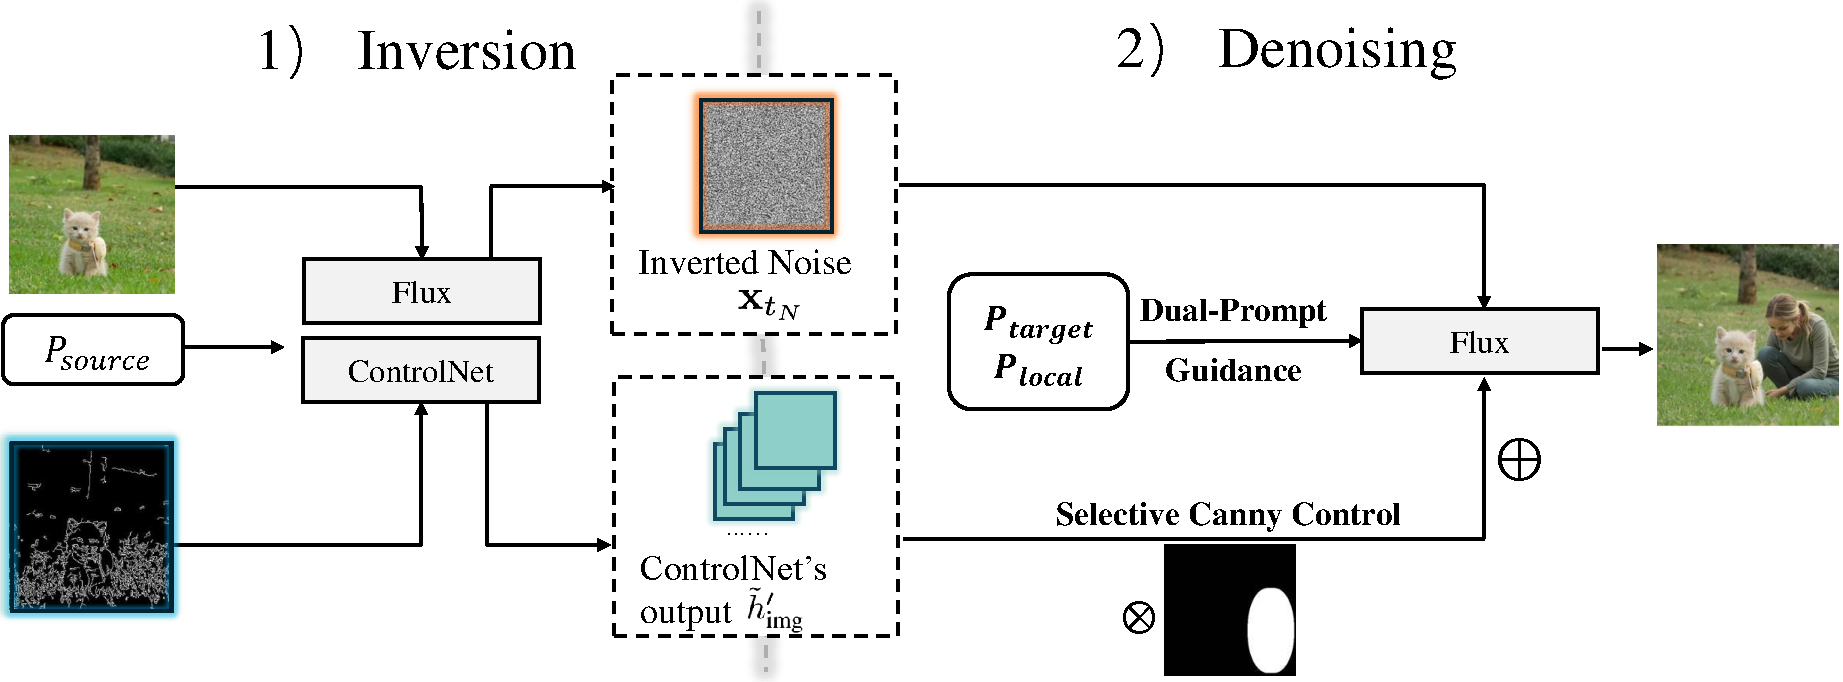
\includegraphics[width=0.8\linewidth]{figures/framework3.pdf}
    \vspace{-1mm}
    \caption{The inversion-denoising process of CannyEdit. 1) \textbf{Inversion}: Starting from the source image, source prompt \( P_\text{source} \), and its Canny edge map, we use FireFlow~\citep{deng2024fireflow} to obtain the inverted noise \( \mathbf{x}_{t_N} \). We also cache the Canny ControlNet outputs \( \tilde{Z}^{\prime}_{\texttt{I}} \) for context preservation. 2) \textbf{Denoising}: Using the inverted noise \( \mathbf{x}_{t_N} \), we perform guided generation with selective Canny control (via a mask), and use local prompts \( P_\text{local} \), and a global target prompt \( P_\text{target} \) to provide multi-level text guidance for editing.}
   % \caption{\textcolor{red}{change notations} The inversion-denoising process of CannyEdit consists of two processes. 1) The inversion process starts with the source image, the source prompt $P_\text{source}$, and the Canny edge map of the source image. With FireFlow \citep{deng2024fireflow}, we transform source image into the inverted noise $\mathbf{x}_{t_N}$. We also cache the Canny ControlNet's outputs $\tilde{Z}^{\prime}_{\texttt{I}}$ for the use of context preservation later. 2) The denoising process starts with the final inverted noise $\mathbf{x}_{t_N}$ from process 1). The additional inputs include the mask for selective Canny control, and local prompts $P_\text{local}$ as well as a global target prompt $P_\text{target}$ for providing multi-level text guidance to the editing.}   %Using model prediction, we transform source image to the inverted noise $\mathbf{x}_{t_N}$. 
   % \caption{The framework of CannyEdit in \textbf{objection insertion task} consists of two process. 1) The inversion process starts with source image (the background), the source prompt $P_\text{source}$, and the Canny edge map of the source image. Using model prediction, we transform source image to the inverted noise. 2) The denoising process starts with the inverted noise from process 1), the Canny edge map of the source image, and additional inputs. The additional inputs include the mask for selective Canny control, and the $P_\text{source}$, $P_\text{target}$, and $P_\text{local}$ for regional text guidance. With denoising process, we transform the inverted noise to the target image.}
    \label{fig:framework}
\end{figure}


%\textcolor{red}{To do: Mention FireFlow and Figure 4 is not precise.}

% The ReFlow ODEs are solved using the Euler method, which is first-order. RFSolver-Edit \citep{wang2024taming} argues that using a second-order solver for ODEs can provide more precise results.
% To reduce computational cost while preserving the precision of the second-order method, Fireflow \citep{deng2024fireflow} proposes to use the midpoint cache from memory. 


%The framework of CannyEdit in \textbf{object insertion task} is shown in Figure \ref{fig:framework}. The frameworks in other tasks, like removal and replacement, are similar to Figure \ref{fig:framework}, with some variances in the textual prompts inputs and mask inputs. More details will be discussed in Sec. \ref{sec:other_tasks}. 







%regional Canny relaxation

% The Canny edge map is a source of guidance for layout preservation. In object insertion task, the background needs to be preserved. Therefore, we always apply Canny control for the background region. However, in object insertion task, the user provides a coarse oval mask indicating the region where the subject should be inserted, and we call it the editable region. In this region, we aim to relax the Canny control as that the target subject can be inserted into the editable region.


\subsection{Selective Canny control}
\label{sec:cannycontrol}

Given a user-provided binary mask \( E \in \{0,1\}^{h \times w} \), where $h \times w$ is the number of image patches, and \( E_{ij} = 1 \) denotes editable regions.  We propose a selective Canny control mechanism that restricts layout guidance to the unedited region while eliminating the guidance signal to the edited region.

This selective control is conducted by selectively masking the Canny ControlNet's outputs before adding them to the FLUX model:
\begin{equation}
Z_{\texttt{I}} \gets Z_{\texttt{I}} + \beta\cdot (1-E) \odot \mathrm{conv}({Z}^{\prime}_{\texttt{I}}).
\label{eq:selective_Canny}
\end{equation}
In the generation of the edited image, ${Z}^{\prime}_{\texttt{I}}$ is the attention output from the Canny edge map tokens, text tokens of the target prompt, and noisy image tokens of the edited image. 

%embedding of the Canny edge map tokens, text tokens of target prompt and the immediate image embedding of the edited image from the FLUX model. 

In the context of image editing, we not only wish to preserve the general layout of the unedited region but also its visual details. In this scenario, the $\tilde{Z}^{\prime}_{\texttt{I}}$ derived from the inversion process serves as a more suitable choice. This is because it includes both the layout information provided by the Canny edge map and the visual features of the source image captured by the noisy image tokens of the source image during the inversion process. We therefore tweak Equation (\ref{eq:selective_Canny}) to:
\begin{equation}
Z_{\texttt{I}} \gets Z_{\texttt{I}} + \beta\cdot (1-E) \odot \mathrm{conv}(\tilde{Z}^{\prime}_{\texttt{I}}).
\label{eq:selective_Canny2}
\end{equation}
The $\tilde{Z}^{\prime}_{\texttt{I}}$ for different denoising blocks across various denoising steps are computed and cached during the inversion process. Thus, the Canny ControlNet can be discarded in the denoising process for efficient consideration. As an optional operation to supplement the background context information provided by $\tilde{Z}^{\prime}_{\texttt{I}}$, when the $\{\mathbf{x}_{t_{1}},...,\mathbf{x}_{t_{N}}\}$ is cached, cyclical blending can be applied to the unedited region:  $\mathbf{x}^\text{edit}_{t_\text{blend}}\gets \alpha\cdot\mathbf{x}^\text{edit}_{t_\text{blend}}+(1-\alpha)\cdot\mathbf{x}_{t_\text{blend}}$ where $t_\text{blend}$ is sampled at a pre-defined frequency.


Besides selectively masking on the edited region, we also propose to reduce the control strength on the mask boundary in the background region by lowering the $\beta$ value according its distance to the center of the mask (details in Appendix A.1). This allows for layout flexibility on the boundary, enabling smooth transitions between edited and unedited regions.  

% While the user-provided mask may not be precise, especially in editing where something new is added to the image, we apply mask refinement via segmentation models \citep{kirillov2023segment,ravi2024sam,medeiros2024langsegmentanything} to obtain the mask of the added object and refine the generation based on this mask (details are in Appendix A.2). This approach helps reduce unnecessary changes to the image context caused by the large mask. 






% $M$ is the mask indicating the editable region which is applied to the ControlNet output. The zero values in $M$ correspond to the background region, and the non-zero values correspond to the editable region. $\odot$ denotes element-wise multiplication.


\subsection{Dual-prompt guidance}
\label{sec:dualprompt}

\subsubsection{General form}
To provide text guidance for directing the text-aligned and seamless editing, we propose a dual-prompt guidance strategy. This approach combines local prompts, which provide region-specific textual signals, with a global target prompt, which incorporates complementary global context by integrating interactions between edited regions and the overall image. While ``dual-prompt'' refers to these two types of prompts, it can involve multiple local prompts to support edits across multiple regions simultaneously. For simplicity, we describe the implementation using two local prompts for providing guidance to two distinct regions, and it can easily extend to the case involving more local prompts.

We denote the two image regions, their corresponding local prompts and global prompt  as $\texttt{I}_\texttt{1}$,  $\texttt{I}_\texttt{2}$,  $\texttt{T}_\texttt{1}$, $\texttt{T}_\texttt{2}$ and $\texttt{T}_\texttt{*}$, respectively, and \sout{the embedding length} \kc{the number of corresponding tokens} is denoted with $|\cdot|$. The query tensor is a concatenated tensor of the image tokens of two image regions and the text tokens of three prompts. We denote the query tensor as the concatenated features $ Q= [Q_{\texttt{I}_\texttt{1}}, Q_{\texttt{I}_\texttt{2}}, Q_{\texttt{T}_\texttt{1}}, Q_{\texttt{T}_\texttt{2}}, Q_{\texttt{T}_\texttt{*}}]$. So are the keys $K$ and values $V$. 

To apply multi-level and multi-region text guidance in a training-free manner, we apply the regional text control via attention mask in  the self-attention module of FLUX blocks (Equation (\ref{eq:FLUX_attention})), which is following prior work \citep{chen2024training}. With the involvement of an attention mask $M$, The attention computation in Equation (\ref{eq:FLUX_attention}) operation is changed to be a masked attention operation:
\begin{equation}
Z = \mathrm{softmax}\left(\frac{QK^\top}{\sqrt{d_k}} \odot M\right)V, \quad\text{where }M = \begin{bmatrix}
        M_{\texttt{I}\to\texttt{I}} &  M_{\texttt{I}\to\texttt{T}} \\
        M_{\texttt{T}\to\texttt{I}} &  M_{\texttt{T}\to\texttt{T}}
    \end{bmatrix}
\label{eq:masked_attention}
\end{equation}
is the attention mask between the concatenated image-text tokens.
% Given the modality correspondence, $ M$ can be denoted as:
% \begin{equation}
    
% \end{equation}
For the text-to-text (T2T) attention, To prevent information leakage of local guidance, each text prompt is restricted to attend only to its own tokens. We enforce this by using a block-diagonal attention mask: $M_{\texttt{T}\to\texttt{T}}=\mathrm{diag}(\mathbf{1}_{|\texttt{T}_\texttt{1}| \times |\texttt{T}_\texttt{1}|}, \mathbf{1}_{|\texttt{T}_\texttt{2}| \times |\texttt{T}_\texttt{2}|},\mathbf{1}_{|\texttt{T}_\texttt{*}| \times|\texttt{T}_\texttt{*}|})$, where the diagonal blocks  in the block-wise diagonal matrix are all-ones matrices that enable full self-attention inside each individual prompt, while all off-diagonal blocks are zero (masked), disabling cross-prompt interactions.


For the attention between the text and the image (T2I), as we intend to use local prompts to provide guidance for specific region, and use a global target prompt to pass the interaction information among different regions, the $M_{\texttt{T}\to\texttt{I}}$ is designed to be:
\begin{equation}
    M_{\texttt{T}\to\texttt{I}} = \begin{bmatrix}
        \mathbf{1}_{|\texttt{T}_\texttt{1}|\times|\texttt{I}_\texttt{1}|} &  \mathbf{0}_{|\texttt{T}_\texttt{1}|\times|\texttt{I}_\texttt{2}|}\\
        \mathbf{0}_{|\texttt{T}_\texttt{2}|\times|\texttt{I}_\texttt{1}|} &  \mathbf{1}_{|\texttt{T}_\texttt{2}|\times|\texttt{I}_\texttt{2}|}\\
         \mathbf{1}_{|\texttt{T}_\texttt{*}|\times|\texttt{I}_\texttt{1}|} &  \mathbf{1}_{|\texttt{T}_\texttt{*}|\times|\texttt{I}_\texttt{2}|}
    \end{bmatrix},
\end{equation}
and symmetrically we let $M_{\texttt{I}\to\texttt{T}}=(M_{\texttt{T}\to\texttt{I}})^\top$, allowing the bidirectional flow of information between the image and text modalities.

For the attention among image tokens (I2I), by default we allow attention only within each region: $M_{\texttt{I}\to\texttt{I}}=\mathrm{diag}(\mathbf{1}_{|\texttt{I}_\texttt{1}| \times |\texttt{I}_\texttt{1}|}, \mathbf{1}_{|\texttt{I}_\texttt{2}| \times |\texttt{I}_\texttt{2}|})$, maintaining the integrity of region-specific edits.

\subsubsection{Tweaking from general form to practical editing tasks}

By default, $M_{\texttt{I}\to\texttt{I}}$ is designed to function as a block-diagonal attention mask when all regions are considered editable. In the practical implementation of editing tasks, this design can be adjusted based on the nature of the regions. For instance, in the case of adding new content where $\texttt{I}_\texttt{1}$ is the edit region and $\texttt{I}_\texttt{2}$ is the background region,
% (e.g., $I_1=I_{bg}$, $I_2=I_{edit}$)
% where we aim to preserve its context,
% the local prompt for the background region could be taken as the source prompt, $T_1=P_\text{source}$.
the local prompt $\texttt{T}_\texttt{2}$ for the background region could be taken as the source prompt.
In this scenario, the $M_{\texttt{I}\to\texttt{I}}$ can be modified as follows:

\begin{equation}
    M_{\texttt{I}\to\texttt{I}}(\texttt{I}_\texttt{1}\to\texttt{I}_\texttt{2})%(\texttt{I}_\texttt{1}, \texttt{I}_\texttt{2})
    % = \mathrm{diag}(\mathbf{1}_{|\texttt{I}_\texttt{1}|^2}, \mathbf{1}_{|\texttt{I}_\texttt{2}|^2})+ \begin{bmatrix}
    %     \mathbf{0}_{|\texttt{I}_\texttt{1}|\times|\texttt{I}_\texttt{1}|} &  \mathbf{0}_{|\texttt{I}_\texttt{1}|\times|\texttt{I}_\texttt{2}|}\\
    %     \mathbf{1}_{|\texttt{I}_\texttt{2}|\times|\texttt{I}_\texttt{1}|} &  \mathbf{0}_{|\texttt{I}_\texttt{2}|\times|\texttt{I}_\texttt{2}|}
    % \end{bmatrix}
    =
    \begin{bmatrix}
        \mathbf{1}_{|\texttt{I}_\texttt{1}|\times|\texttt{I}_\texttt{1}|} &  \mathbf{1}_{|\texttt{I}_\texttt{1}|\times|\texttt{I}_\texttt{2}|}\\
        \mathbf{0}_{|\texttt{I}_\texttt{2}|\times|\texttt{I}_\texttt{1}|} &  \mathbf{1}_{|\texttt{I}_\texttt{2}|\times|\texttt{I}_\texttt{2}|}
    \end{bmatrix},
    \label{eq:i2i_1}
\end{equation}

where we additionally allow the edit region $\texttt{I}_\texttt{1}$ to attend to the background region $\texttt{I}_\texttt{2}$ through $\mathbf{1}_{|\texttt{I}_\texttt{1}|\times|\texttt{I}_\texttt{2}|}$. This adjustment allows the model to integrate contextual information from the background region into the edited region, allowing the more context-aware edit. This masking approach can also be simply extended to multiple editable regions while preserving the background.

% To seamlessly blend the edited and background regions, we further refine the I2I attention related to the background region near the boundary of the edited part. The region is denoted as $\texttt{I}_\texttt{:}$ and the region not in the boundary as ${I}_{\text{bg(nbd)}}$. Define the $M_{\texttt{I}\to\texttt{I}}(\texttt{I}_\texttt{1},\texttt{I}_\texttt{:}, \texttt{I}_\texttt{2})$ as:
% \begin{equation}
% M_{\texttt{I}\to\texttt{I}}(\texttt{I}_\texttt{1},\texttt{I}_\texttt{:}, \texttt{I}_\texttt{2}) =   \begin{bmatrix}
%         \mathbf{1}_{|\texttt{I}_\texttt{1}|\times|\texttt{I}_\texttt{1}|} &  \mathbf{1}_{|\texttt{I}_\texttt{1}|\times|\texttt{I}_\texttt{:}|}&\mathbf{0}_{|\texttt{I}_\texttt{1}|\times|\texttt{I}_\texttt{2}|}\\

% \mathbf{1}_{|\texttt{I}_\texttt{:}|\times|\texttt{I}_\texttt{1}|} &  \mathbf{1}_{|\texttt{I}_\texttt{:}|\times|\texttt{I}_\texttt{:}|}&\boxed{\mathbf{1}_{|\texttt{I}_\texttt{:}|\times|\texttt{I}_\texttt{2}|}}\\
% \mathbf{1}_{|\texttt{I}_\texttt{2}|\times|\texttt{I}_\texttt{1}|} &  \mathbf{1}_{|\texttt{I}_\texttt{2}|\times|\texttt{I}_\texttt{:}|}&\mathbf{1}_{|\texttt{I}_\texttt{2}|\times|\texttt{I}_\texttt{2}|}\\
%     \end{bmatrix}.
% \label{eq:i2i_2}
% \end{equation}
To seamlessly blend the edited and background regions, we further refine the I2I attention related to the background region near the boundary of the edited part. The region is denoted as $\texttt{I}_\texttt{:}$ and the background region not at the boundary as $\texttt{I}_\texttt{2}$. Define $M_{\texttt{I}\to\texttt{I}}(\texttt{I}_\texttt{1}\to\texttt{I}_\texttt{2};\  \texttt{I}_\texttt{1}\leftrightarrow\texttt{I}_\texttt{:}\!\leftrightarrow \texttt{I}_\texttt{2})$ as:
\begin{equation}
M_{\texttt{I}\to\texttt{I}}(\texttt{I}_\texttt{1}\to\texttt{I}_\texttt{2};\  \texttt{I}_\texttt{1}\leftrightarrow\texttt{I}_\texttt{:}\!\leftrightarrow \texttt{I}_\texttt{2}) =   \begin{bmatrix}
        \mathbf{1}_{|\texttt{I}_\texttt{1}|\times|\texttt{I}_\texttt{1}|} &  \mathbf{1}_{|\texttt{I}_\texttt{1}|\times|\texttt{I}_\texttt{:}|}&\mathbf{1}_{|\texttt{I}_\texttt{1}|\times|\texttt{I}_\texttt{2}|}\\

\boxed{\mathbf{1}_{|\texttt{I}_\texttt{:}|\times|\texttt{I}_\texttt{1}|}} &  \mathbf{1}_{|\texttt{I}_\texttt{:}|\times|\texttt{I}_\texttt{:}|}&\mathbf{1}_{|\texttt{I}_\texttt{:}|\times|\texttt{I}_\texttt{2}|}\\
\mathbf{0}_{|\texttt{I}_\texttt{2}|\times|\texttt{I}_\texttt{1}|} &  \mathbf{1}_{|\texttt{I}_\texttt{2}|\times|\texttt{I}_\texttt{:}|}&\mathbf{1}_{|\texttt{I}_\texttt{2}|\times|\texttt{I}_\texttt{2}|}\\
    \end{bmatrix}.
\label{eq:i2i_2}
\end{equation}
The change from Equation (\ref{eq:i2i_1}) to Equation (\ref{eq:i2i_2}) lies in the boxed block $\mathbf{1}_{|\texttt{I}_\texttt{:}|\times|\texttt{I}_\texttt{1}|}$.
With this modification, background region on the boundary of the mask region can now attends to the edit region,  enabling the model to  incorporate contextual cues from the edited region into the boundary areas. As a result, the boundary areas can better align visually and semantically with the edits, reducing artifacts and improving the overall coherence of the image.

% This approach can be simply extended to multiple editable regions while preserving the background:
% \begin{equation*}
% M_{\texttt{I}\to\texttt{I}} = {\mathrm{diag}}(\mathbf{1}_{|\texttt{I}_\texttt{1}|^2}, \mathbf{1}_{|I_{\text{edit1}}|^2}, \dots, \mathbf{1}_{|I_{\text{editn}}|^2}) + \begin{bmatrix}
% \mathbf{0}_{|\texttt{I}_\texttt{1}|\times|I_\text{edit1}|} & \mathbf{0}_{|\texttt{I}_\texttt{1}|\times|I_\text{edit2}|} & \dots & \mathbf{0}_{|\texttt{I}_\texttt{1}|\times|I_\text{editn}|} \\
% \mathbf{1}_{|I_\text{edit1}|\times|\texttt{I}_\texttt{1}|} & \mathbf{0}_{|I_\text{edit1}|\times|I_\text{edit2}|} & \dots & \mathbf{0}_{|I_\text{edit1}|\times|I_\text{editn}|} \\
% \vdots & \vdots & \ddots & \vdots \\
% \mathbf{1}_{|I_\text{editn}|\times|\texttt{I}_\texttt{1}|} & \mathbf{0}_{|I_\text{editn}|\times|I_\text{edit2}|} & \dots & \mathbf{0}_{|I_\text{editn}|\times|I_\text{editn}|}
% \end{bmatrix}
% \end{equation*}
\subsubsection{Prompting for different editing tasks}

The local prompts vary across different editing tasks. In addition and replacement tasks, the local prompts specify the objects to be added or those replacing the existing ones. For removal tasks, we default to using ``empty background" as the local prompt. To more effectively remove existing objects, we employ class-free guidance \citep{ho2022classifier}, incorporate descriptions of the target objects to be removed as negative local prompts, A more detailed introduction of how these techniques can be applied to different editing tasks, such as object transfer with preserved object shapes or modification on the environment or atmosphere of a specific region is provided in \textcolor{red}{Appendix B}. The Appendix also delves into how our method can be extended to handle multiple edits in a single generation pass.

%thereby improving their suppression during editing.
% Furthermore, the local prompts used in different editing tasks differ. In the adding and replacement task, the local prompts represent the objects to add or to replace the existing objects. In the removal task, we use ``empty background'' as the local prompt by default. To more effectively eliminate existing objects, we apply class-free guidance \citep{ho2022classifier}, which incorporates descriptions of the target removal objects as negative local prompts, thereby enhancing their suppression during the editing process. The more details of the application of our proposed techniques to different editing tasks are given in \textcolor{red}{Appendix B}.

% The application of the techniques to other editing tasks, like in the replacement and removal, requires some other minor tweaking. For instance, in the replacement and removal, there is no readily available description for the background region (the source prompt is not aligned with the background region), we do not apply a local prompt for the background area and only apply local prompts to the edit area. The local 


% $M_{\texttt{T}\to\texttt{T}}$ ignored;
% only write $M_{\texttt{I}\to\texttt{I}}$ and $M_{\texttt{I}\to\texttt{I}}$

%\textcolor{red}{involving two mask notation $M$ and $M$, how to connect or distinguish them.}

% To apply multi-level and multi-region text guidance, we apply Region-Aware Attention \citep{xxx} in the self-attention module of FLUX blocks (Equation (\ref{eq:FLUX_attention})). The query tensor is a concatenated tensor of the image tokens of two image regions and the text tokens of three prompts. We denote the query tensor as the concatenated features $ Q= [Q_{I_A}, Q_{I_B}, Q_{P_A}, Q_{P_B}, Q_{P_{AB}}]$. So are the keys $K$ and values $V$. The masked attention operation becomes:


% $ M$ is a self-attention mask between the concatenated image-text features. Given the modality correspondence, $ M$ can be denoted as:

% \begin{equation}
%     M = \begin{bmatrix}
%         M_{\texttt{I}\to\texttt{I}} &  M_{I2P} \\
%         M_{P2I} &  M_{P2P} 
%     \end{bmatrix}
% \end{equation}

% Suppose the text tokens lengths of $P_A$, $P_B$, and $P_{AB}$ are denoted by $L_{P_A}$, $L_{P_B}$, $L_{P_{AB}}$, we can write $M_{P2P}$ as:

% \begin{equation}
%     M_{P2P} = \mathrm{diag}(\mathbf{1}_{L_{P_A}\times L_{P_A}}, \mathbf{1}_{L_{P_B} \times L_{P_B}}, \mathbf{1}_{L_{P_{AB}} \times L_{P_{AB}}})
% \end{equation}

% This text-to-text attention mask prevents information leakage among different text prompts. $\mathbf{1}_L$ is an all-ones matrix with shape $L \times L$.

% Suppose the image tokens lengths of $I_A$, $I_B$ are denoted by $L_{I_A}$, $L_{I_B}$, we write $M_{P2I}$ as:

% \begin{equation}
%     M_{P2I} = \begin{bmatrix}
%         \mathrm{diag}(\mathbf{1}_{L_{P_A} \times L_{I_A}}, \mathbf{1}_{L_{P_B} \times L_{I_B}})  \\
%         \mathbf{1}_{L_{P_{AB}} \times (L_{I_{A}} + L_{I_{B}})}
%     \end{bmatrix}
% \end{equation}

% $\mathrm{diag}(\mathbf{1}_{L_{P_A} \times L_{I_A}}, \mathbf{1}_{L_{P_B} \times L_{I_B}})$ indicates the local prompt tokens only attend to the local image tokens with correspondence: $P_A \rightarrow I_A$ and $P_B \rightarrow I_B$. $\mathbf{1}_{L_{P_{AB}} \times (L_{I_{A}} + L_{I_{B}})}$ indicates that the global prompt tokens attend to every region: $P_{AB} \rightarrow I_A, I_B$.  $M_{I2P}$ follows the symmetric correspondence, therefore, $M_{I2P} =  M_{P2I}^\top$.


% \begin{equation}
%     M_{\texttt{I}\to\texttt{I}} = \mathrm{diag}(\mathbf{1}_{L_{I_A}\times L_{I_A}}, \mathbf{1}_{L_{I_B} \times L_{I_B}})  + \begin{bmatrix}
%          \mathbf{0}_{L_{I_A}\times L_{I_A}} & \mathbf{0}_{L_{I_A}\times L_{I_B}} \\
%          \mathbf{1}_{L_{I_A}\times L_{I_B}}  & \mathbf{0}_{L_{I_B}\times L_{I_B}} 
%     \end{bmatrix}
%     \label{eq:i2i_attention_mask}
% \end{equation}

% The first term in Equation (\ref{eq:i2i_attention_mask}) indicates that image tokens only attend to each other within each region. However, we allow information leakage from the non-editable region to editable region for better affordance. Therefore, we introduce the second term in Equation (\ref{eq:i2i_attention_mask}). This allows information leakage from region $A$ to region $B$, but not in the reverse direction.

% In object insertion task, $P_A$ is the source prompt describing the background region $I_A$, $P_B$ is the local prompt describing the subject to be inserted in the editable region $I_B$. Finally, the target prompt is the global prompt $P_{AB}$ describing the whole target image.


% \subsection{Extensions to other tasks} \label{sec:other_tasks}
% \begin{table}[h!]
% \centering
% \caption{The mask and prompts inputs for different image editing tasks}
%  \vskip 1em
% \resizebox{\textwidth}{!}{%
% \begin{tabular}{l l l}
% \toprule
% Task & Mask for Canny Control & Prompts for Regional Guidance \\
% \midrule
% Object Insertion & coarse mask or &  $P_\text{source} \leftrightarrow I_{non-edit}$,\\
%  & segmentation mask  &  $P_\text{local} \leftrightarrow I_{edit}$,  $P_\text{target} \leftrightarrow  [I_{non-edit}, I_{edit}]$  \\\midrule 

% Object Replacement & segmentation mask & $P_\text{local} \leftrightarrow I_{edit}$,  $P_\text{target} \leftrightarrow [ I_{non-edit}, I_{edit}]$   \\  \midrule
% Object Removal & segmentation mask  & Positive prompts:  \\
% & & \text{"empty background"} $\leftrightarrow I_{edit}$, $P_\text{target} \leftrightarrow  [I_{non-edit}, I_{edit}]$  \\  
% & & Negative prompts:  \\
% & &  $P_\text{local} \leftrightarrow I_{edit}$,  $P_\text{source} \leftrightarrow  [I_{non-edit}, I_{edit}]$ \\ 

% \bottomrule
% \end{tabular}}
% \label{tab:tasks}
% \end{table}



% Our method is naturally extendable to other image editing tasks, like object replacement and object removal. In both tasks, the target object to be edited needs to be located and segmented ahead. We used out-of-box instance segmentation tool, Language SAM \citep{xx}, to get the segmentation mask of the target object. More details about extracting segmentation masks can be found in Appendix.


% Table \ref{tab:tasks} lists the mask and prompts inputs for different image editing tasks. The object insertion task can accept a coarse mask (brush-like or oval mask) or a refined segmentation mask for selective Canny control, and three prompts for regional text guidance. 

% \subsubsection{Object replacement}

%  For the object replacement task, the source prompt is only used in the inversion process, not applied in the denoising process. In other words, we only use the local prompt and the target prompt for regional text guidance.

 
% %\subsection{Object transfer with full Canny control}

% %\textcolor{red}{Examples (Figure \ref{fig2}) to showcase that direct regional control cannot make edits. However, selective Canny masking can allow the local editability.}


% %\subsection{Regional image editing with selective Canny control}

% % \subsubsection{Object adding with mask refinement}

% % Preservation of original information in edited region
% % Mask acquisition of the generated objects
% % Synthetic Canny
% % Cyclical blending 
% %To allow the generation of collateral objects but maintain the background mainly unchanged, we do the cyclical blending with partial blending on the background region with the inversion latent.

% \subsubsection{Object removal}

% We use classifier-free guidance (CFG) for the object removal task. The positive prompts consist of a default local prompt (i.e., "empty background") and a target prompt. The negative prompts consist of the local prompt and the source prompt. 


% \subsubsection{Personalization with copy-paste synthesis}
% %\subsection{Extension to different tasks}


%
%\subsection{Cyclic blending}
%\label{sec:blend}
%% 


% \begin{table}[h!]
% \centering
% \caption{Technical Summary}
%  \vskip 1em
% \resizebox{\textwidth}{!}{%
% \begin{tabular}{l l l l l}
% \toprule
% Task & Definition & Inputs & Canny Guidance & Regional Control\\
% \midrule
% Object Transfer & Replace an object with another, & source prompt, target prompt, local prompt,  & full Canny control& target prompt - whole image,  \\
%  & preserving the original shape or structure. & source image + mask of object to be replaced. & & local prompt - edit region. \\ \midrule
% Replacement &Replace an object with another, & source prompt, target prompt, local prompt, & selective Canny masking& target prompt - whole image,  \\
% & \textbf{without} preserving the original shape or structure. & source image + mask of object to be replaced. & &local prompt - edit region.  \\\midrule
% Context Change & Modify the environment or atmosphere of a specific region,&source prompt, target prompt, local prompt, &selective Canny weakening  & target prompt - whole image, \\
% & like changing clouds to rain or making the sky sunny.& source image + mask of  environment to be changed. & &local prompt - edit region.  \\ \midrule
% Adding &Introduce a new object into a specific region of the scene.  &source prompt, target prompt, local prompt,   &selective Canny masking & target prompt - whole image,   \\
% &&source image + a rough mask for region of added object to be added. & &source prompt - BG region, local prompt - edit region. \\\midrule
% Removal & Remove a specific object from the scene.& source prompt, target prompt, & selective Canny masking &  {Pos.}:  target prompt - whole image, \\
%  & & neg. local prompt, (pos. local prompt), &   & pos. local prompt (default, `empty background') - edit region; \\

%  && source image + mask of object to be removed.&&Neg.: source prompt - whole image, neg. local prompt - edit region. \\\midrule



% Copy-paste Synthesis & Make the affordance-aware copy-pasted object insertion. & source prompt, target prompt, local prompt,& synthesis Canny control +  & target prompt - whole image,\\
%  & &source image + synthesis image w/ reference object pasted. &selective Canny masking & source prompt - BG region, local prompt - edit region.\\
% \bottomrule
% \end{tabular}}
% \label{tab:tasks}
% \end{table}





\section{Experiments}
\label{Sec:experiment}


\subsection{Experimental setup}

\textbf{Baselines.} Two kinds of methods are compared with CannyEdit: (1) Training-based approaches including BrushEdit~\cite{li2024brushedit} based on UNet diffusion models, FLUX Fill~\cite{blackforest2024FLUX} and PowerPaint-FLUX~\cite{zhuang2023task} based on FLUX~\cite{blackforest2024FLUX}. Note that the original PowerPaint in \cite{blackforest2024FLUX} is based on UNet diffusion model, for a fairer comparison, we trained a new version based on FLUX with the provided training dataset. (2) Training-free approaches including P2P~\cite{hertz2022prompt}, MasaCtrl~\cite{cao2023masactrl} based on DDIM \citep{song2022denoisingdiffusionimplicitmodels}, and RF-Inversion~\cite{rout2024semantic}, RFSolver-Edit~\cite{wang2024taming}, KV-Edit~\cite{zhu2025kv} based on Rectified
Flow. %In summary, there are eight prevalent image inpainting and editing methods for evaluation. 

\textbf{Datasets.} We introduce the \textbf{R}eal \textbf{I}mage \textbf{C}omplex \textbf{E}diting Benchmark ({RICE-Bench}) to address the lack of realistic interactions among objects in existing real-world image editing benchmarks~\citep{sheynin2024emu,gu2024multi}. RICE-Bench consists of 80 images depicting real scenes and complex editing scenarios for adding, replacement, and removal tasks. It is designed to better evaluate \textit{context fidelity}, \textit{text adherence}, and \textit{editing seamlessness} in real-world editing tasks. Example images from the benchmark are shown in \textcolor{red}{FigureXX}, with details of data curation provided in \textcolor{red}{AppendixXX}. We also conduct evaluations on PIE-Bench~\cite{ju2024pnp}, a dataset of 620 real-world and synthetic images spanning 9 diverse editing tasks, excluding the style transfer task to focus on region-based image editing, consistent with \cite{li2024brushedit, xu2023infedit, zhu2025kv}.

%In this work, we focus on real-world image editing scenarios that involve complex interactions between the edited region and the surrounding image context. However, existing real-world image benchmarks~\citep{sheynin2024emu,gu2024multi} primarily involve edits to minor objects and lack realistic interactions among objects (e.g., ``add a glass of water on the table''). To address this limitation, we introduce the \textbf{R}eal \textbf{I}mage \textbf{C}omplex \textbf{E}diting Benchmark ({RICE-Bench}), designed to better evaluate \textit{context fidelity}, \textit{text adherence}, and \textit{editing seamlessness} in real-world editing tasks. RICE-Bench consists of 80 images depicting real scenes and complex editing scenarios for adding, replacement and removal tasks (the 15 adding examples used for the quantitative study in Figure \ref{fig2}(a) are a subset of the RICE-Bench). Example images from the benchmark are shown in \textcolor{red}{Figure~XX}, with details of the data curation and additional samples provided in \textcolor{red}{Appendix~XX}. Following prior works, we conduct evaluations on PIE-Bench~\cite{ju2024pnp}, a dataset of 620 real-world and synthetic images spanning 9 diverse editing tasks. Consistent with \cite{li2024brushedit, xu2023infedit, zhu2025kv}, we exclude the style transfer task from our evaluation, as our focus is on region-based image editing.

\textbf{Implementation Details.} We implement our method based on FLUX.1-[dev]\cite{blackforest2024FLUX} and FLUX-Canny-ControlNet\cite{xlabsai2025fluxcontrolnet}, using 50 denoising steps and a guidance value of 4.0. The strength parameter of Canny control $\beta$ is set to 0.8 in the inversion and for the non-mask-boundary background region. We apply cyclical blending with $\alpha=0.5$ every 5 steps. Other methods were implemented based on their official code releases' default settings unless otherwise specified. More details, including machines used, hyperparameters, and a computational cost analysis for CannyEdit, are provided in \textcolor{red}{Appendix C}.
% \textbf{Implementation Details.} We implement our method based on FLUX.1-[dev]~\cite{blackforest2024FLUX} and FLUX-Canny-ControlNet~\cite{xlabsai2025fluxcontrolnet}. Most hyperparameters are consistent with FLUX-Canny-ControlNet, using 50 denoising steps and guidance value as 4.0. The strength parameter of Canny control $\beta$ is set to be 0.8 in the inversion and for the background region not in the boundary of the mask region. We apply the cyclical blending with $\alpha=0.5$ in a frequency of every 5 steps. The implementation of other methods was based on the default settings in their official code releases unless otherwise specified. More implementation details, including the machines used and the detailed hyperparameters, are provided in \textcolor{red}{Appendix C}. An analysis of the computational cost for CannyEdit is also provided in the same appendix. %In short, compared to previous training-free methods based on FLUX \cite{rout2024semantic,wang2024taming}, our method does not involve significant computational overhead.

%For RICE-Bench, we resize images to resolution of 1024, while 512 in PIE-Bench.

%\textbf{Metrics.} For RICE-Bench, we evaluate edits using three metrics: \textbf{Context Fidelity (CF)}, \textbf{Text Adherence (TA)}, and \textbf{Trade-off Score (TO Score)}. CF measures the cosine similarity between the DINO embeddings~\citep{caron2021emerging} of the original and edited images. TA quantifies how well the edited image follows the text prompts via GroundingDINO~\citep{liu2024grounding} top-1 bounding-box prediction confidence for the specified object, $p_{\text{gdino}}(\textit{image}, \textit{object name})$. For {addition} and {replacement} edits, $\text{TA} = p_{\text{gdino}}(\textit{edited}, A) - p_{\text{gdino}}(\textit{source}, A)$ where $\textit{edited}$/$\textit{source}$  denote edited/source image and $A$ is the object to be added or to replace existing objects, while for {removal} edits, $\text{TA} = p_{\text{gdino}}(\textit{source}, A) - p_{\text{gdino}}(\textit{edited}, A)$ where $A$ is the object to be removed.  TO Score assesses the balance between editability and fidelity, calculated as $\text{TO Score} = \text{CF} + \text{TA}$. A user study was conducted based on RICE-Bench to evaluate editing seamlessness by comparing the extent to which users can discern AI-edited results. For PIE-Bench, following \citet{zhu2025kv}, we report seven metrics: HPSv2 \citep{wu2023human} and aesthetic scores \citep{schuhmann2022laionb} for image quality; PSNR \citep{huynh2008scope}, LPIPS \citep{zhang2018perceptual}, and MSE for background preservation accuracy; and CLIP score \citep{radford2021learning} and Image Reward \citep{xu2023imagereward} for text adherence.


% \textbf{Metrics.}  For RICE-Bench, we evaluate edits using three metrics: \textbf{Context Fidelity (CF)}, \textbf{Text Adherence (TA)}, and \textbf{Trade-off Score (TO Score)}. CF measures cosine similarity between original and edited images using DINO embeddings~\citep{caron2021emerging}. TA assesses adherence to text prompts via GroundingDINO~\citep{liu2024grounding} top-1 bounding-box prediction confidence for the edited object, defined as the confidence difference between edited and source images (positive for addition/replacement edits, reversed for removal edits to measure the successful elimination of the object). TO Score balances fidelity and editability, computed as $\text{TO Score} = \text{CF} + \text{TA}$. RICE-Bench also includes a user study evaluating editing seamlessness by gauging users' ability to identify AI-generated edits. For PIE-Bench, following \citet{zhu2025kv}, we use seven metrics: HPSv2~\citep{wu2023human} and aesthetic scores~\citep{schuhmann2022laionb} (image quality), PSNR~\citep{huynh2008scope}, LPIPS~\citep{zhang2018perceptual}, and MSE (background preservation), and CLIP score~\citep{radford2021learning} and Image Reward~\citep{xu2023imagereward} (text adherence).

\textbf{Metrics.}  For RICE-Bench, we evaluate edits using three metrics: \textbf{Context Fidelity (CF)}, \textbf{Text Adherence (TA)}, and \textbf{Trade-off Score (TO Score)}. CF measures cosine similarity between original and edited images using DINO embeddings~\citep{caron2021emerging}. TA assesses adherence to text prompts via GroundingDINO~\citep{liu2024grounding} top-1 bounding-box prediction confidence $p_{\text{gdino}}(\textit{image}, \textit{edited object})$ for the edited object, defined as the confidence difference between edited and source images: positive in $p_{\text{gdino}}(\textit{edited}, \textit{edited object})-p_{\text{gdino}}(\textit{source}, \textit{removed object})$ for addition/replacement edits and reversed in $p_{\text{gdino}}(\textit{source}, \textit{removed object})-p_{\text{gdino}}(\textit{edited}, \textit{removed object})$ for removal edits to measure the successful elimination of the object. TO Score balances fidelity and editability, computed as $\text{TO Score} = \text{CF} + \text{TA}$. RICE-Bench also includes a user study evaluating editing seamlessness by gauging users' ability to identify AI-generated edits. For PIE-Bench, following \citet{zhu2025kv}, we use seven metrics: HPSv2~\citep{wu2023human} and aesthetic scores~\citep{schuhmann2022laionb} (image quality), PSNR~\citep{huynh2008scope}, LPIPS~\citep{zhang2018perceptual}, and MSE (background preservation), and CLIP score~\citep{radford2021learning} and Image Reward~\citep{xu2023imagereward} (text adherence).

% \textbf{Metrics.} For RICE-Bench, we evaluate edits using two primary metrics: \textbf{context fidelity (CF)} and  \textbf{Text Adherence (TA)}. CF is quantified by calculating the cosine similarity between the DINO embeddings~\citep{caron2021emerging} of the original and edited images. TA measures how successfully the edited image follows the provided textual instruction, utilizing GroundingDINO~\citep{liu2024grounding} bounding-box prediction confidence. Specifically, for {addition} and {replacement} editing (where subject \(A\) is inserted into or replaces an existing subject, TA is computed as: $\text{TA} = p_{\text{gdino}}(\textit{edited}, A) - p_{\text{gdino}}(\textit{source}, A)$ where \(p_{\text{gdino}}(\text{image}, A)\) indicates GroundingDINO's~\citep{liu2024grounding} top-1 bounding-box probability for the subject \(A\). For {removal} instructions (where subject \(A\) is to be removed from the image), TA is inversely defined as: $\text{TA} = p_{\text{gdino}}(\textit{source}, A) - p_{\text{gdino}}(\textit{edited}, A)$. Additionally, we introduce the \textbf{Trade-off Score (TO Score)} to comprehensively assess the balance between editability and fidelity, calculated as the sum of CF and TA: $\text{TO Score} = \text{CF} + \text{TA}$. To evaluate the editing seamlessness, we designed and conducted a user study comparing the extent to which users can discern whether results from different methods have been edited by AI.

%based on editing results from different methods and ground-truth editing results (a subset of evaluation source images (30) is created by manually removing a subject from the image and thus the target image 




\subsection{Experiment results on RICE-bench}



\begin{table*}[t]
\begin{center} 
\footnotesize
\setlength{\tabcolsep}{1.70mm} %
\caption{{Results of Automatically computed metrics comparing with representative methods on RICE-Bench.} The  ``inject'' for RFSolver-Edit denotes the number of denoising steps where the source image's attention features are injected. The metrics are context fidelity (CF), Text Adherence (TA) and Trade-off Score (TO Score) which measures the trade-off for editability and fidelity. \textbf{Bold} and \underline{underlined} values represent the best and second-best TO scores respectively.}

\resizebox{0.95\textwidth}{!}{
\begin{tabular}{lcccccccccc}
\toprule
 & \multicolumn{3}{c}{Add} & \multicolumn{3}{c}{Removal} &\multicolumn{3}{c}{Replace} & Avg.\\
\cmidrule(lr){2-4} \cmidrule(lr){5-7} \cmidrule(lr){8-10} \cmidrule(lr){11-11}
Metrics & $\textup{CF}_{\times 10^2}^{\uparrow}$ & $\textup{TA}_{\times 10^2}^{\uparrow}$ & TO Score& $\textup{CF}_{\times 10^2}^{\uparrow}$ & $\textup{TA}_{\times 10^2}^{\uparrow}$ & TO Score& $\textup{CF}_{\times 10^2}^{\uparrow}$ & $\textup{TA}_{\times 10^2}^{\uparrow}$ & TO Score& TO Score\\
\midrule
RFSolver-Edit ($\textup{inject}=2$)~\cite{wang2024taming} & 71.77 & 22.65 & 94.42 & 42.99 & 39.05 & 82.04 & 47.44 & 9.22 & 56.66 & 77.71\\
RFSolver-Edit ($\textup{inject}=8$)~\cite{wang2024taming} & 99.13 & 2.14 & 101.27 & 79.34 & 2.94 & 82.28 & 67.89 & 5.03 & 72.92 & 85.49\\
KV-Edit~\cite{zhu2025kv} & 93.91 & 17.25 & \underline{111.16} & 69.81 & 16.62 & 86.43 & 64.72 & 12.36 & \underline{77.08} & \underline{91.56}\\
BrushEdit~\cite{li2024brushedit} & 87.26 & 18.98 & 106.24 & 63.43 & 31.29 & \underline{94.72} & 59.11 & 7.40 & 66.51 & 89.16\\
FLUX Fill~\cite{blackforest2024FLUX} & 88.21 & 21.62 & 109.83 & 70.94 & 10.91 & 81.85 & 60.20 & 8.13 & 68.33 & 86.67\\
Powerpaint-FLUX~\cite{zhuang2023task} & 84.63 & 24.34 & 108.97 & 62.31 & 21.40 & 83.71 & 60.75 & 8.92 & 69.67 & 87.45\\
\midrule
\textbf{CannyEdit (Ours)} & 88.72 & 28.12 & \textbf{116.84} & 63.28 & 34.22 & \textbf{97.50} & 64.43 & 16.77 & \textbf{81.20} & \textbf{98.51}\\
\bottomrule
\end{tabular}}
\label{tab:rice-comparison}
\end{center}

\begin{center} 
\footnotesize
\setlength{\tabcolsep}{1.85mm} %
\caption{{Results of user study comparing with representative methods on RICE-Bench ({\scriptsize $\pm${}} represents 95\% confidence interval).}   In Task~1, AI-generated images (\emph{Gen}) and real, unedited images (\emph{Real}) are paired to ask which image has been edited by AI. Seamless edits should yield pick ratios close to the random choices (i.e., 50\%), which can be witnessed in our CannyEdit. In Task~2, CannyEdit's results are paired with those from other methods. Lower ratios for ``ours'' indicate the better editing seamelessness of our methods.}

\

\resizebox{1.\textwidth}{!}{
\begin{tabular}{lcccccccc}
\toprule
 & \multicolumn{4}{c}{General Public (96 participants)} & \multicolumn{4}{c}{Expert (41 participants)} \\
 \cmidrule(lr){2-5}\cmidrule(lr){6-9}
%\midrule
& \multicolumn{2}{c}{{Generated vs. Real}} & \multicolumn{2}{c}{CannyEdit vs. Others} &\multicolumn{2}{c}{Generated vs. Real} & \multicolumn{2}{c}{CannyEdit vs. Others}\\
%\midrule
 \cmidrule(lr){2-3} \cmidrule(lr){4-5}\cmidrule(lr){6-7}\cmidrule(lr){8-9}
 Ratio regarded as AIGC (\%) & $\textup{Gen}^{\downarrow}$ & $\textup{Real}^{\uparrow}$ & $\textup{Ours}^{\downarrow}$ & $\textup{Itself}^{\downarrow}$ & $\textup{Gen}^{\downarrow}$ & $\textup{Real}^{\uparrow}$ & $\textup{Ours}^{\downarrow}$ & $\textup{Itself}^{\downarrow}$\\
\midrule
%Random choices & 50.00  & 50.00 & 50.00 & 50.00 & 50.00 & 50.00 & 50.00 & 50.00\\
%\midrule
KV-Edit~\cite{zhu2025kv} & 86.96{\scriptsize $\pm${7.19}}  & 13.04{\scriptsize $\pm${7.19}} & \textbf{37.50}{\scriptsize $\pm${5.72}} & 62.50{\scriptsize $\pm${5.72}} & 89.09{\scriptsize $\pm${9.24}} & 10.91{\scriptsize $\pm${9.24}} & \textbf{37.69}{\scriptsize $\pm${10.2}} & 62.31{\scriptsize $\pm${10.2}}\\
BrushEdit~\cite{li2024brushedit} & 79.20{\scriptsize $\pm${8.99}} & 20.80{\scriptsize $\pm${8.99}} & \textbf{30.00}{\scriptsize $\pm${4.90}} & 70.00{\scriptsize $\pm${4.90}} & \underline{82.00}{\scriptsize $\pm${12.1}} & \underline{18.00}{\scriptsize $\pm${12.1}} & \textbf{19.29}{\scriptsize $\pm${9.99}} & 80.71{\scriptsize $\pm${9.99}}\\
Powerpaint-FLUX~\cite{zhuang2023task} & \underline{76.08}{\scriptsize $\pm${5.49}} & \underline{23.92}{\scriptsize $\pm${5.49}} & \textbf{38.08}{\scriptsize $\pm${6.66}} & 61.92{\scriptsize $\pm${6.66}} & 88.00{\scriptsize $\pm${6.57}} & 12.00{\scriptsize $\pm${6.57}} & \textbf{33.85}{\scriptsize $\pm${7.32}} & 66.15{\scriptsize $\pm${7.32}}\\
\midrule
\textbf{CannyEdit (Ours)} & \textbf{49.20}{\scriptsize $\pm${3.56}} & \textbf{50.80}{\scriptsize $\pm${3.56}} & N/A & N/A & \textbf{42.00}{\scriptsize $\pm${8.12}} & \textbf{58.00}{\scriptsize $\pm${8.12}} & N/A & N/A\\
\bottomrule
\end{tabular}}
\label{tab:rice-human-study} 
\end{center}
\end{table*}

Table~\ref{tab:rice-comparison} compares our method with others using automatic metrics. Achieving the highest TO score across three editing tasks, our method demonstrates the best balance between editability and fidelity. RFSolver-Edit either attains high text adherence but disrupts image context with fewer feature injection steps, or preserves context but fails to apply the desired edits with more steps. KV-Edit preserves context better but at the cost of considerably lower text adherence. Training-based methods also struggle to achieve a comparable balance.

Moreover, We conducted a simple yet effective user study to systematically evaluate the editing seamlessness of different methods. A total of 137 participants were recruited and divided into two groups: the general public (96 first-year undergraduates with no AIGC background) and experts (41 participants with formal AIGC training or experience).

The study consisted of two tasks. In each, participants were shown two images and asked to answer the following question: \emph{``Please select the image (a) or (b) you believe is most likely to have been edited by an AI model''}. The tasks differ from the image pairs provided: \textbf{Task 1:} An AI-edited image was compared with a real, unedited image; \textbf{Task 2:} An image generated by CannyEdit was compared with the one from another editing method, using the same source image and editing instruction. To reduce bias, image and question order were randomized, and each participant saw 20 randomly selected questions. Only successfully edited examples (with high TA scores) were included in the study. A screening test ensured data quality: participants were required to evaluate 10 individual images (including images from different editing methods and unedited real images) as AI-edited or real, and those with poor accuracy (correct rate <50\%) were excluded (2 from the public group). Further study details are provided in \textcolor{red}{Appendix D}.

As shown in Table~\ref{tab:rice-human-study}, participants in Task 1 had difficulty distinguishing CannyEdit outputs from real, unedited images. When presented alongside real-world images without edits, the general public identified CannyEdit images as AI-edited only 49.20\% of the time, while experts did so at an even lower rate of 42.00\%. In contrast, images produced by alternative methods were more frequently flagged as AI-generated, with detection rates ranging from 76.08\% to 89.09\%. Similarly, in Task 2, CannyEdit-generated images were consistently less likely to be recognized as AI-edited compared to those from other methods, highlighting the superior seamlessness of CannyEdit's editing capabilities.

% As shown in Table~\ref{tab:rice-human-study}, in Task1, participants struggled to distinguish CannyEdit outputs from real images, with   49.20\% for the general public and 42.00\% for experts to considered as AI-edited when paired with a real-world image without edits. In contrast, images from other methods were identified as AI-edited more frequently, with rates ranging from 76.08\% to 89.09\%. In Task2, CannyEdit images were consistently less likely to be flagged as AI-edited compared to those from other methods, demonstrating its superior editing seamlessness.

% As shown in Table~\ref{tab:rice-human-study}, in Task~1, participants struggled to distinguish CannyEdit outputs from real images (AI pick rates: 49.20\% for the general public, 42.00\% for experts), while images from other methods were identified as AI-edited more frequently (76.08\%--89.09\%). In Task~2, CannyEdit images were consistently less likely to be flagged as AI-edited than those from other methods, demonstrating its superior editing seamlessness.

% Table~\ref{tab:rice-comparison} presents a comparison with other methods using automatically computed metrics. As indicated by the best TO score, our method significantly improves the balance of the editability-fidelity trade-off overall. For other methods, RFSolver-Edit either follows the text prompt well with a high TA but fundamentally changes the image context with a significantly low CF when injecting two steps of the source image's features, or maintains the image context well but fails to make the desired edit when injecting more steps. KV-Edit maintains a better CF but at the cost of a significantly worse TA. The training-based methods also fall short of maintaining a good balance compared to ours.

%we present comparison with other methods in automatically computed metrics. Across three editing tasks, CannyEdit can maintain a high-level of CF while TA achieves the best in Add and Replace, and second in Removal. Although a variant(inject=2) of RFSolver-Edit is the first in TA, it has a poor corresponding performance of CF, which indicates that it generates many samples having little connection with original image. To better measure the trade-off between editability and fidelity, we sum up CF and TA across three tasks as the TO score. Clearly, CannyEdit saliently outperforms others with a new level of balance.

% Moreover, we designed a simple yet effective user study to systematically evaluate the editing seamlessness of different methods.  In total, we recruited 137 participants, divided into two groups: the general public group (96 participants) and the expert group (41 participants). The general public group consisted of first-year undergraduate students from a university, with no technical background in AI-Generated Content (AIGC). The expert group comprised individuals who at least had either studied AIGC models in a credit-bearing course or trained an AIGC-related model.

% The user study involve two tasks. In both tasks, the participants were provided two images and asked the same question \emph{``Please select the image (a) or (b) you believe is most likely to have been edited by an AI model.''}. For Task 1 (AI-edited vs. real-world images), each question provided an AI-edited image and a real-world image without edits. Task 2 (CannyEdit vs. another AI editing method) presented a pair of images, one generated by CannyEdit and the other by a different editing method, using the same source image and editing instruction. To minimize order bias, we randomized the image order in the questions, the question order in both tasks, and users were shown 20 random questions. Only examples with successful editing, as indicated by high $\text{TA}$, were included. To ensure study quality, we included a screening test before tasks 1 and 2. Users were shown 10 images (a mix of AI-edited and real-world images) and asked if each was AI-edited. Two participants from the general public group were excluded for having a correct ratio below 50\% on real-world images. Further details, including the study interface, are provided in \textcolor{red}{Appendix C}.

% The results in Table~\ref{tab:rice-human-study} show that in Task 1, participants in both groups had difficulty differentiating CannyEdit-generated images from real-world images, choosing almost randomly (pick ratio of AI-edited is 49.20\% and 42.00\%, respectively). In contrast, images from other methods were more likely to be identified as AI-edited (76.08\%-89.09\%). For Task 2, CannyEdit's outputs were consistently less likely to be regarded as AI-edited compared to other methods' ouptuts. These results demonstrate that CannyEdit achieves significantly seamless editing performance.

%The results in Table~\ref{tab:rice-human-study} show that in both groups, participants almost randomly give choices between images generated by CannyEdit and real-world images, which demonstrates it is hard for users to differentiate edited images by our method from real images. In contrast, results from other methods have a much higher ratio of picking as AI-edited (76.08\%-89.09\%) For Task 2, compared to results from other evaluated methods, the outputs from our CannyEdit are all less likely to be regarded as AI-edited by the users. All the results elucidate that CannyEdit achieves a significant performance of seamlessness. 

%based on editing results from different methods and ground-truth editing results (a subset of evaluation source images (30) is created by manually removing a subject from the image and thus the target image 


% basic knowledge. Each group is asked to finish the same two tasks. For Task 1, each question randomly sampling a pair of images, which includes a generated(Gen) sample by different editing methods and a ground-truth(GT) real image respectively. The participant needs to answer which one has been more likely edited by an AI model. In Task 2, different from previous one, a pair of images consists of a sample generated by CannyEdit (our method) and a sample from other editing methods based on the same source image and editing instruction. The participant should choose which one has been more likely edited by an AI model. Such a design can help participants concentrate more on intuitive visual sensation rather than worry about additional semantic information utilized in \cite{zhu2025kv}, which deteriorates stability of feedback. \textcolor{red}{Some examples of question are shown in Appendix.}


 

\subsection{Experiment results on PIE-bench}

\begin{table*}[t]

\begin{center} 
\footnotesize
\setlength{\tabcolsep}{1.85mm} %
\caption{{Comparison with other methods on PIE-Bench.} VAE$^*$ denotes the inherent reconstruction error through VAE reconstruction only. Except the result of ours, other results follow \cite{zhu2025kv}.}
\resizebox{0.8\textwidth}{!}{
\begin{tabular}{lccccccc}
\toprule
\multirow{3}{*}[0.8ex]{Metrics} & \multicolumn{2}{c}{Image Quality} & \multicolumn{3}{c}{Masked Region Preservation} &\multicolumn{2}{c}{Text Adherence} \\
\cmidrule(lr){2-3}\cmidrule(lr){4-6}\cmidrule(lr){7-8}   &  $\textup{HPS}_{\times 10^2}^{\uparrow}$ & $\textup{AS}^{\uparrow}$ & $\textup{PSNR}^\uparrow$ & $\textup{LPIPS}_{\times 10^3}^{\downarrow}$ & $\textup{MSE}_{\times 10^4}^{\downarrow}$ & $\textup{CLIP Sim}^{\uparrow}$ & $\textup{IR}_{\times10}^{\uparrow}$\\
\midrule
VAE$^*$ & 24.93 & 6.37 & 37.65 & 7.93 & 3.86 & 19.69 & -3.65\\
\midrule
P2P~\cite{hertz2022prompt} & 25.40 & 6.27& 17.86 & 208.43 & 219.22 & 22.24 & 0.017 \\
MasaCtrl~\cite{cao2023masactrl} & 23.46 & 5.91 & 22.20 & 105.74 & 86.15 & 20.83 & -1.66\\
RF-Inversion~\cite{rout2024semantic} & \textbf{27.99} & \textbf{6.74} & 20.20 & 179.73 & 139.85 & 21.71 & 4.34\\
RFSolver-Edit~\cite{wang2024taming} & \underline{27.60} & \underline{6.56}& 24.44& 113.20& 56.26& 22.08& 5.18\\
KV-Edit~\cite{zhu2025kv} & 27.21 & 6.49 & \textbf{35.87}& \textbf{9.92}& \textbf{4.69}& 22.39 & 5.63\\
BrushEdit~\cite{li2024brushedit} & 25.81 & 6.17 & 32.16 & \underline{17.22} & \underline{8.46} & \underline{22.44} & 3.33\\
FLUX Fill~\cite{blackforest2024FLUX} & 25.76 & 6.31 & \underline{32.53} & 25.59 & 8.55 & 22.40 & \underline{5.71}\\
%Powerpaint-FLUX~\cite{zhuang2023task} & & & & & & & \\
\midrule
\textbf{CannyEdit (Ours)} & 27.19 & 6.38 & 32.18 & 26.38 & 9.79& \textbf{25.36} & \textbf{8.20}\\
\bottomrule
\end{tabular}}
\label{tab:pie-comparison} 
\end{center}

\begin{center} 
\footnotesize
\setlength{\tabcolsep}{1.05mm} %
\caption{{Ablation study for CannyEdit on adding and replacement examples of RICE-Bench.} The evaluation metrics follow these in Table \ref{tab:rice-comparison}. \emph{CC} denotes Canny Control, \emph{DP} is for Dual-Prompt Guidance and  \emph{CB} means cyclical blending. For comparison, we also copy the results of KV-Edit here.}

\

\resizebox{0.7\textwidth}{!}{
\begin{tabular}{llcccccc}
\toprule
&  & \multicolumn{3}{c}{Add} & \multicolumn{3}{c}{Replace}\\
\cmidrule(lr){3-5}\cmidrule(lr){6-8}
 & & $\textup{CF}_{\times 10^2}^{\uparrow}$ & $\textup{TA}_{\times 10^2}^{\uparrow}$ & $\textup{TO Score}^{\uparrow}$ & $\textup{CF}_{\times 10^2}^{\uparrow}$ & $\textup{TA}_{\times 10^2}^{\uparrow}$ & $\textup{TO Score}^{\uparrow}$ \\
\midrule
% Baseline & w/o CC, w/o Rx & 81.4/22.0 & 103.4 & ---- & ---- & 48.7/14.9 & 63.6 \\
KV-Edit (baseline) && 93.91 & 17.25 & 111.16 &64.72&12.36&77.08 \\\midrule
\textbf{CannyEdit (Ours)} &  &{88.72} &{28.12} & \textbf{116.8} & {64.43}&{16.77} & \textbf{81.20} \\
\midrule
\multirow{3}{*}{\begin{tabular}[c]{@{}c@{}}Variants \\ \arraybackslash of CC\end{tabular}} & 
selective CC w/ Eq.(\ref{eq:selective_Canny})   &84.81 &27.93 &112.74 &55.2&13.9x  & 69.1   \\
&w/o CC & 79.73&{26.29} & 106.02 & 51.5&11.8 & 63.3 \\
 & full CC  & {93.41}&19.73 & {113.14} & {68.1}&10.5 & {78.6} \\
\midrule
\multirow{2}{*}{\begin{tabular}[c]{@{}c@{}}Variants \\ \arraybackslash of DP\end{tabular}} & local prompt only  & {93.43}&10.23 & 103.66 & 58.9&{17.1} & 76.0 \\
 & target prompt only& 85.04&24.96 & 109.00& 60.8&15.4 & 76.2 \\
\midrule 
Variant of CB &blend at every step & 93.24&22.09&115.33 &67.4&11.0 & 78.4\\
\bottomrule
\end{tabular}}
\label{tab:ablation-study} 
\end{center}
\end{table*}

% \begin{figure}[htbp]
%     \centering
%     % First image pair
%     \begin{subfigure}[b]{0.2\textwidth}
%         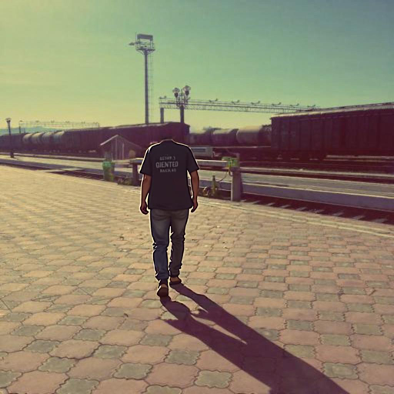
\includegraphics[width=\linewidth]{figures/tm/image1.png}
%         \caption*{(a.1)}
%     \end{subfigure}
%     \begin{subfigure}[b]{0.2\textwidth}
%         \includegraphics[width=\linewidth]{figures/tm/image2.png}
%         \caption*{(a.2)}
%     \end{subfigure}
%     % Second image pair
%     \begin{subfigure}[b]{0.2\textwidth}
%         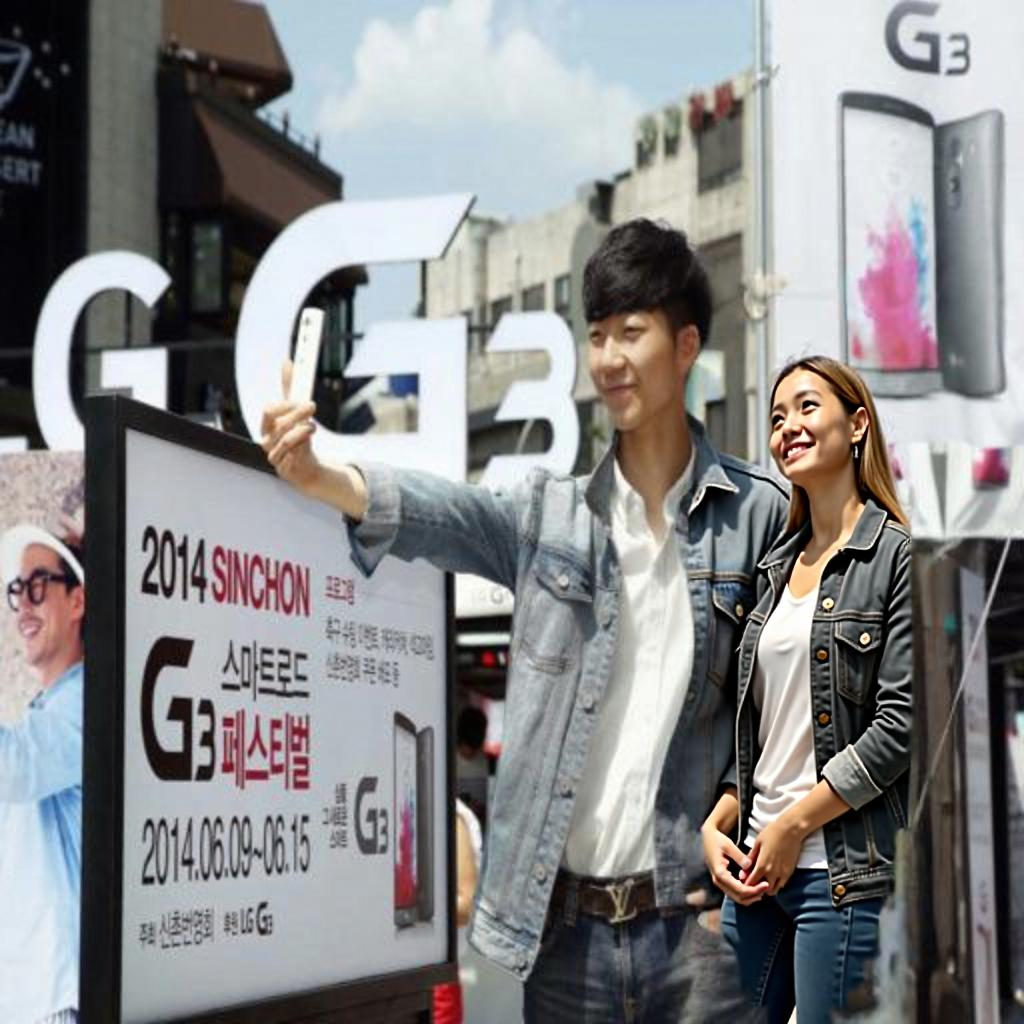
\includegraphics[width=\linewidth]{figures/tm/3941.jpeg}
%         \caption*{(b.1)}
%     \end{subfigure}
%     \begin{subfigure}[b]{0.2\textwidth}
%         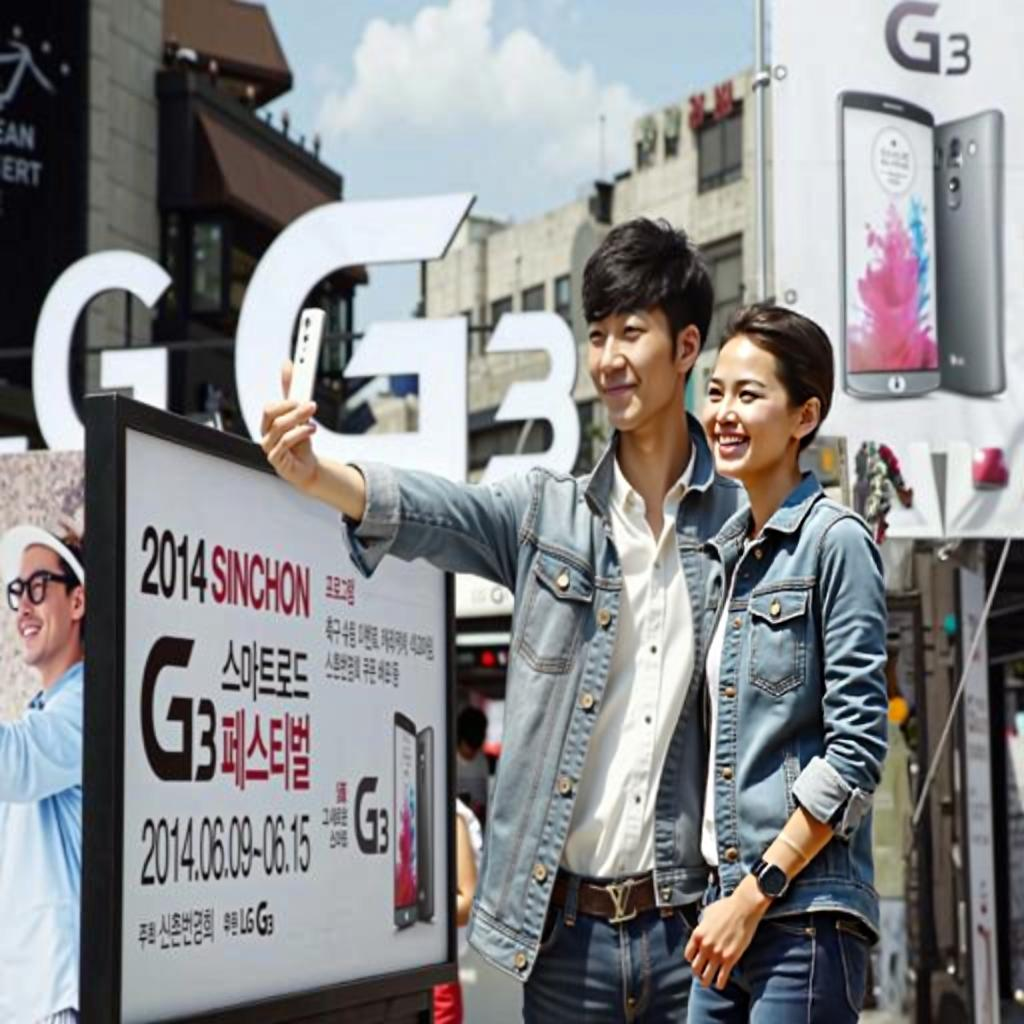
\includegraphics[width=\linewidth]{figures/tm/image5.jpeg}
%         \caption*{(b.2)}
%     \end{subfigure}
%     \caption{Visual examples highlight the importance of special treatments at the boundary between edited and unedited regions. Without treatments, (a.1) and (b.1) show rough transitions, while (a.2) and (b.2) demonstrate smoother results with treatments of reduced canny control and attention adjustment applied.}
%     \label{fig:treaments}
% \end{figure}


Besides, we further expand evaluation to PIE-bench, including more number of images and editing tasks. The result is displayed in Table~\ref{tab:pie-comparison}. As for text alignment, CannyEdit significantly outperforms other methods both in CLIP similarity($22.44\rightarrow \textbf{25.36}$) and Image Reward($5.71\rightarrow \textbf{8.20}$). At the same time, our method also keeps a competitive level in image quality and masked region preservation. 

\subsection{Ablation study}

We validate the effectiveness of key modules in CannyEdit based on adding and replacement examaples in RICE-Bench.  As shown in Table~\ref{tab:ablation-study}, not using cached ControlNet outputs (i.e., applying selective Canny control from Equation~(\ref{eq:selective_Canny})) or omitting Canny control during image generation leads to a noticeable drop in context fidelity. In contrast, applying full Canny control throughout the process improve context preservation but significantly weakens the model's ability to follow the textual editing instructions.  Furthermore, ablations on the dual-prompt guidance indicate that both local prompts and the global target prompt play vital roles in achieving successful edits. CannyEdit also introduces cyclic blending, which merges background features from the original image at a fixed frequency. Although blending at every denoising step better preserves image context, it compromises adherence to the text instructions and reduces editing precision. 

% In the adding task, we apply mask refinement via segmentation models to avoid the change on other objects covered in the user-provided masks. The results of with and without mask refinement in Table~\ref{tab:ablation-study} show that the mask refinement can help with the preservation of image context better. While it would lead to minor desreament on the text adherence, it still lead to a better overall trade-off.


%Mention results of using VLM to estimate masks

CannyEdit introduces special treatments for the boundary region between edited and unedited areas to ensure a smoother visual transition, using reduced Canny control and attention attending to the edited region. Figure \ref{fig:treaments} illustrates the importance of these treatments—without them, noticeable artifacts and unnatural transitions appear at the boundaries. Additional visual examples of various ablations are provided in \textcolor{red}{Appendix G}. For this evaluation and examples shown in the paper, we use an oval-shaped mask for adding by default. In \textcolor{red}{Appendix H}, we further demonstrate that CannyEdit remains robust to different mask shapes, including rectangular and user-drawn styles.

\subsection{Qualitative examples}

\textcolor{red}{In Figure xx, }





Mention results of multiple edits at one pass in Appendix F (show two or three in Figure 1)

Mention results of other editing tasks in Appendix F

Mention results of comparison with GPT-4o and Gemini in Appendix F


% we display some qualitative examples comparing CannyEdit with RFSolver-Edit and KV-Edit, which have higher value in the two aspects. It is clear that samples generated by our method is better aligned with target prompts while having no irrational change in unedited regions from source images.[supplement qualitative samples






%Examples of hard blending every step: collateral effects, more examples of ablation study in Appendix xx




% In this section, we validate effectiveness of key modules in CannyEdit based on Editing tasks Add and Replace in RICE-Bench. Following Table~\ref{tab:ablation-study}, it shows that selective Canny Control(CC) with features corresponding to edited regions masked, outperforms full CC or without CC in terms of Trade-off Score($106.0\rightarrow \textbf{116.8}$). Then, Regional Text guidance(Rx) composing both local prompt within mask and target prompt globally, improves a lot compared with only local prompt or target prompt($109.9\rightarrow \textbf{114.1}$). What's more, Rx also enhances robustness facing unprecise masks, which narrow the gap between results of original mask and with mask refinement($114.1\leftrightarrow 116.8$ for Rx, and $109.9\leftrightarrow 103.6$ for local prompt only).


\section{Conclusion}

\section{Limitations and future improvements}
\label{Sec:limitation}
1. Eliminate the needs of input masks: Use VLM to infer the region to apply Canny masking or weakening;
2. Support different kinds of controls (like pose control in local region, depth control and multiple conditions)? 
3. Interactive editing?
4. Extend to more models.

% \section{Submission of papers to NeurIPS 2025}




% Please read the instructions below carefully and follow them faithfully.


% \subsection{Style}


% Papers to be submitted to NeurIPS 2025 must be prepared according to the
% instructions presented here. Papers may only be up to {\bf nine} pages long,
% including figures.
% % Additional pages \emph{containing only acknowledgments and references} are allowed.
% Additional pages \emph{containing references, checklist, and the optional technical appendices} do not count as content pages.
% Papers that exceed the page limit will not be
% reviewed, or in any other way considered for presentation at the conference.


% The margins in 2025 are the same as those in previous years.


% Authors are required to use the NeurIPS \LaTeX{} style files obtainable at the
% NeurIPS website as indicated below. Please make sure you use the current files
% and not previous versions. Tweaking the style files may be grounds for
% rejection.


% \subsection{Retrieval of style files}


% The style files for NeurIPS and other conference information are available on
% the website at
% \begin{center}
%   \url{https://neurips.cc}
% \end{center}
% The file \verb+neurips_2025.pdf+ contains these instructions and illustrates the
% various formatting requirements your NeurIPS paper must satisfy.


% The only supported style file for NeurIPS 2025 is \verb+neurips_2025.sty+,
% rewritten for \LaTeXe{}.  \textbf{Previous style files for \LaTeX{} 2.09,
%   Microsoft Word, and RTF are no longer supported!}


% The \LaTeX{} style file contains three optional arguments: \verb+final+, which
% creates a camera-ready copy, \verb+preprint+, which creates a preprint for
% submission to, e.g., aRxiv, and \verb+nonatbib+, which will not load the
% \verb+natbib+ package for you in case of package clash.


% \paragraph{Preprint option}
% If you wish to post a preprint of your work online, e.g., on aRxiv, using the
% NeurIPS style, please use the \verb+preprint+ option. This will create a
% nonanonymized version of your work with the text ``Preprint. Work in progress.''
% in the footer. This version may be distributed as you see fit, as long as you do not say which conference it was submitted to. Please \textbf{do
%   not} use the \verb+final+ option, which should \textbf{only} be used for
% papers accepted to NeurIPS.


% At submission time, please omit the \verb+final+ and \verb+preprint+
% options. This will anonymize your submission and add line numbers to aid
% review. Please do \emph{not} refer to these line numbers in your paper as they
% will be removed during generation of camera-ready copies.


% The file \verb+neurips_2025.tex+ may be used as a ``shell'' for writing your
% paper. All you have to do is replace the author, title, abstract, and text of
% the paper with your own.


% The formatting instructions contained in these style files are summarized in
% Sections \ref{gen_inst}, \ref{headings}, and \ref{others} below.


% \section{General formatting instructions}
% \label{gen_inst}


% The text must be confined within a rectangle 5.5~inches (33~picas) wide and
% 9~inches (54~picas) long. The left margin is 1.5~inch (9~picas).  Use 10~point
% type with a vertical spacing (leading) of 11~points.  Times New Roman is the
% preferred typeface throughout, and will be selected for you by default.
% Paragraphs are separated by \nicefrac{1}{2}~line space (5.5 points), with no
% indentation.


% The paper title should be 17~point, initial caps/lower case, bold, centered
% between two horizontal rules. The top rule should be 4~points thick and the
% bottom rule should be 1~point thick. Allow \nicefrac{1}{4}~inch space above and
% below the title to rules. All pages should start at 1~inch (6~picas) from the
% top of the page.


% For the final version, authors' names are set in boldface, and each name is
% centered above the corresponding address. The lead author's name is to be listed
% first (left-most), and the co-authors' names (if different address) are set to
% follow. If there is only one co-author, list both author and co-author side by
% side.


% Please pay special attention to the instructions in Section \ref{others}
% regarding figures, tables, acknowledgments, and references.


% \section{Headings: first level}
% \label{headings}


% All headings should be lower case (except for first word and proper nouns),
% flush left, and bold.


% First-level headings should be in 12-point type.


% \subsection{Headings: second level}


% Second-level headings should be in 10-point type.


% \subsubsection{Headings: third level}


% Third-level headings should be in 10-point type.


% \paragraph{Paragraphs}


% There is also a \verb+\paragraph+ command available, which sets the heading in
% bold, flush left, and inline with the text, with the heading followed by 1\,em
% of space.


% \section{Citations, figures, tables, references}
% \label{others}


% These instructions apply to everyone.


% \subsection{Citations within the text}


% The \verb+natbib+ package will be loaded for you by default.  Citations may be
% author/year or numeric, as long as you maintain internal consistency.  As to the
% format of the references themselves, any style is acceptable as long as it is
% used consistently.


% The documentation for \verb+natbib+ may be found at
% \begin{center}
%   \url{http://mirrors.ctan.org/macros/latex/contrib/natbib/natnotes.pdf}
% \end{center}
% Of note is the command \verb+\citet+, which produces citations appropriate for
% use in inline text.  For example,
% \begin{verbatim}
%    \citet{hasselmo} investigated\dots
% \end{verbatim}
% produces
% \begin{quote}
%   Hasselmo, et al.\ (1995) investigated\dots
% \end{quote}


% If you wish to load the \verb+natbib+ package with options, you may add the
% following before loading the \verb+neurips_2025+ package:
% \begin{verbatim}
%    \PassOptionsToPackage{options}{natbib}
% \end{verbatim}


% If \verb+natbib+ clashes with another package you load, you can add the optional
% argument \verb+nonatbib+ when loading the style file:
% \begin{verbatim}
%    \usepackage[nonatbib]{neurips_2025}
% \end{verbatim}


% As submission is double blind, refer to your own published work in the third
% person. That is, use ``In the previous work of Jones et al.\ [4],'' not ``In our
% previous work [4].'' If you cite your other papers that are not widely available
% (e.g., a journal paper under review), use anonymous author names in the
% citation, e.g., an author of the form ``A.\ Anonymous'' and include a copy of the anonymized paper in the supplementary material.


% \subsection{Footnotes}


% Footnotes should be used sparingly.  If you do require a footnote, indicate
% footnotes with a number\footnote{Sample of the first footnote.} in the
% text. Place the footnotes at the bottom of the page on which they appear.
% Precede the footnote with a horizontal rule of 2~inches (12~picas).


% Note that footnotes are properly typeset \emph{after} punctuation
% marks.\footnote{As in this example.}


% \subsection{Figures}


% \begin{figure}
%   \centering
%   \fbox{\rule[-.5cm]{0cm}{4cm} \rule[-.5cm]{4cm}{0cm}}
%   \caption{Sample figure caption.}
% \end{figure}


% All artwork must be neat, clean, and legible. Lines should be dark enough for
% purposes of reproduction. The figure number and caption always appear after the
% figure. Place one line space before the figure caption and one line space after
% the figure. The figure caption should be lower case (except for first word and
% proper nouns); figures are numbered consecutively.


% You may use color figures.  However, it is best for the figure captions and the
% paper body to be legible if the paper is printed in either black/white or in
% color.


% \subsection{Tables}


% All tables must be centered, neat, clean and legible.  The table number and
% title always appear before the table.  See Table~\ref{sample-table}.


% Place one line space before the table title, one line space after the
% table title, and one line space after the table. The table title must
% be lower case (except for first word and proper nouns); tables are
% numbered consecutively.


% Note that publication-quality tables \emph{do not contain vertical rules.} We
% strongly suggest the use of the \verb+booktabs+ package, which allows for
% typesetting high-quality, professional tables:
% \begin{center}
%   \url{https://www.ctan.org/pkg/booktabs}
% \end{center}
% This package was used to typeset Table~\ref{sample-table}.


% \begin{table}
%   \caption{Sample table title}
%   \label{sample-table}
%   \centering
%   \begin{tabular}{lll}
%     \toprule
%     \multicolumn{2}{c}{Part}                   \\
%     \cmidrule(r){1-2}
%     Name     & Description     & Size ($\mu$m) \\
%     \midrule
%     Dendrite & Input terminal  & $\sim$100     \\
%     Axon     & Output terminal & $\sim$10      \\
%     Soma     & Cell body       & up to $10^6$  \\
%     \bottomrule
%   \end{tabular}
% \end{table}

% \subsection{Math}
% Note that display math in bare TeX commands will not create correct line numbers for submission. Please use LaTeX (or AMSTeX) commands for unnumbered display math. (You really shouldn't be using \$\$ anyway; see \url{https://tex.stackexchange.com/questions/503/why-is-preferable-to} and \url{https://tex.stackexchange.com/questions/40492/what-are-the-differences-between-align-equation-and-displaymath} for more information.)

% \subsection{Final instructions}

% Do not change any aspects of the formatting parameters in the style files.  In
% particular, do not modify the width or length of the rectangle the text should
% fit into, and do not change font sizes (except perhaps in the
% \textbf{References} section; see below). Please note that pages should be
% numbered.


% \section{Preparing PDF files}


% Please prepare submission files with paper size ``US Letter,'' and not, for
% example, ``A4.''


% Fonts were the main cause of problems in the past years. Your PDF file must only
% contain Type 1 or Embedded TrueType fonts. Here are a few instructions to
% achieve this.


% \begin{itemize}


% \item You should directly generate PDF files using \verb+pdflatex+.


% \item You can check which fonts a PDF files uses.  In Acrobat Reader, select the
%   menu Files$>$Document Properties$>$Fonts and select Show All Fonts. You can
%   also use the program \verb+pdffonts+ which comes with \verb+xpdf+ and is
%   available out-of-the-box on most Linux machines.


% \item \verb+xfig+ "patterned" shapes are implemented with bitmap fonts.  Use
%   "solid" shapes instead.


% \item The \verb+\bbold+ package almost always uses bitmap fonts.  You should use
%   the equivalent AMS Fonts:
% \begin{verbatim}
%    \usepackage{amsfonts}
% \end{verbatim}
% followed by, e.g., \verb+\mathbb{R}+, \verb+\mathbb{N}+, or \verb+\mathbb{C}+
% for $\mathbb{R}$, $\mathbb{N}$ or $\mathbb{C}$.  You can also use the following
% workaround for reals, natural and complex:
% \begin{verbatim}
%    \newcommand{\RR}{I\!\!R} %real numbers
%    \newcommand{\Nat}{I\!\!N} %natural numbers
%    \newcommand{\CC}{I\!\!\!\!C} %complex numbers
% \end{verbatim}
% Note that \verb+amsfonts+ is automatically loaded by the \verb+amssymb+ package.


% \end{itemize}


% If your file contains type 3 fonts or non embedded TrueType fonts, we will ask
% you to fix it.


% \subsection{Margins in \LaTeX{}}


% Most of the margin problems come from figures positioned by hand using
% \verb+\special+ or other commands. We suggest using the command
% \verb+\includegraphics+ from the \verb+graphicx+ package. Always specify the
% figure width as a multiple of the line width as in the example below:
% \begin{verbatim}
%    \usepackage[pdftex]{graphicx} ...
%    \includegraphics[width=0.8\linewidth]{myfile.pdf}
% \end{verbatim}
% See Section 4.4 in the graphics bundle documentation
% (\url{http://mirrors.ctan.org/macros/latex/required/graphics/grfguide.pdf})


% A number of width problems arise when \LaTeX{} cannot properly hyphenate a
% line. Please give LaTeX hyphenation hints using the \verb+\-+ command when
% necessary.

% \begin{ack}
% Use unnumbered first level headings for the acknowledgments. All acknowledgments
% go at the end of the paper before the list of references. Moreover, you are required to declare
% funding (financial activities supporting the submitted work) and competing interests (related financial activities outside the submitted work).
% More information about this disclosure can be found at: \url{https://neurips.cc/Conferences/2025/PaperInformation/FundingDisclosure}.


% Do {\bf not} include this section in the anonymized submission, only in the final paper. You can use the \texttt{ack} environment provided in the style file to automatically hide this section in the anonymized submission.
% \end{ack}





\newpage
\bibliography{main}
\bibliographystyle{plainnat}




%%%%%%%%%%%%%%%%%%%%%%%%%%%%%%%%%%%%%%%%%%%%%%%%%%%%%%%%%%%%

% \appendix

% \section{Technical Appendices and Supplementary Material}
% Technical appendices with additional results, figures, graphs and proofs may be submitted with the paper submission before the full submission deadline (see above), or as a separate PDF in the ZIP file below before the supplementary material deadline. There is no page limit for the technical appendices.

%%%%%%%%%%%%%%%%%%%%%%%%%%%%%%%%%%%%%%%%%%%%%%%%%%%%%%%%%%%%

\newpage
\section*{NeurIPS Paper Checklist}

\begin{enumerate}

\item {\bf Claims}
    \item[] Question: Do the main claims made in the abstract and introduction accurately reflect the paper's contributions and scope?
    \item[] Answer: \answerYes{} % Replace by \answerYes{}, \answerNo{}, or \answerNA{}.
    \item[] Justification: We pinpoint the area we are in and list contributions clearly. Please refer to Abstract and Introduction \ref{Sec:intro}.
    \item[] Guidelines:
    \begin{itemize}
        \item The answer NA means that the abstract and introduction do not include the claims made in the paper.
        \item The abstract and/or introduction should clearly state the claims made, including the contributions made in the paper and important assumptions and limitations. A No or NA answer to this question will not be perceived well by the reviewers. 
        \item The claims made should match theoretical and experimental results, and reflect how much the results can be expected to generalize to other settings. 
        \item It is fine to include aspirational goals as motivation as long as it is clear that these goals are not attained by the paper. 
    \end{itemize}

\item {\bf Limitations}
    \item[] Question: Does the paper discuss the limitations of the work performed by the authors?
    \item[] Answer: \answerYes{} % Replace by \answerYes{}, \answerNo{}, or \answerNA{}.
    \item[] Justification: We clarify datasets used in experiment section \ref{Sec:experiment}. Also, we discuss the limitations in section \ref{Sec:limitation}.
    \item[] Guidelines:
    \begin{itemize}
        \item The answer NA means that the paper has no limitation while the answer No means that the paper has limitations, but those are not discussed in the paper. 
        \item The authors are encouraged to create a separate "Limitations" section in their paper.
        \item The paper should point out any strong assumptions and how robust the results are to violations of these assumptions (e.g., independence assumptions, noiseless settings, model well-specification, asymptotic approximations only holding locally). The authors should reflect on how these assumptions might be violated in practice and what the implications would be.
        \item The authors should reflect on the scope of the claims made, e.g., if the approach was only tested on a few datasets or with a few runs. In general, empirical results often depend on implicit assumptions, which should be articulated.
        \item The authors should reflect on the factors that influence the performance of the approach. For example, a facial recognition algorithm may perform poorly when image resolution is low or images are taken in low lighting. Or a speech-to-text system might not be used reliably to provide closed captions for online lectures because it fails to handle technical jargon.
        \item The authors should discuss the computational efficiency of the proposed algorithms and how they scale with dataset size.
        \item If applicable, the authors should discuss possible limitations of their approach to address problems of privacy and fairness.
        \item While the authors might fear that complete honesty about limitations might be used by reviewers as grounds for rejection, a worse outcome might be that reviewers discover limitations that aren't acknowledged in the paper. The authors should use their best judgment and recognize that individual actions in favor of transparency play an important role in developing norms that preserve the integrity of the community. Reviewers will be specifically instructed to not penalize honesty concerning limitations.
    \end{itemize}

\item {\bf Theory assumptions and proofs}
    \item[] Question: For each theoretical result, does the paper provide the full set of assumptions and a complete (and correct) proof?
    \item[] Answer: \answerNA{} % Replace by \answerYes{}, \answerNo{}, or \answerNA{}.
    \item[] Justification: We don't have theoretical results.
    \item[] Guidelines:
    \begin{itemize}
        \item The answer NA means that the paper does not include theoretical results. 
        \item All the theorems, formulas, and proofs in the paper should be numbered and cross-referenced.
        \item All assumptions should be clearly stated or referenced in the statement of any theorems.
        \item The proofs can either appear in the main paper or the supplemental material, but if they appear in the supplemental material, the authors are encouraged to provide a short proof sketch to provide intuition. 
        \item Inversely, any informal proof provided in the core of the paper should be complemented by formal proofs provided in appendix or supplemental material.
        \item Theorems and Lemmas that the proof relies upon should be properly referenced. 
    \end{itemize}

    \item {\bf Experimental result reproducibility}
    \item[] Question: Does the paper fully disclose all the information needed to reproduce the main experimental results of the paper to the extent that it affects the main claims and/or conclusions of the paper (regardless of whether the code and data are provided or not)?
    \item[] Answer: \answerYes{} % Replace by \answerYes{}, \answerNo{}, or \answerNA{}.
    \item[] Justification: We elucidate datasets used, baselines to compare, and implementation details of our method in section \ref{Sec:experiment}.
    \item[] Guidelines:
    \begin{itemize}
        \item The answer NA means that the paper does not include experiments.
        \item If the paper includes experiments, a No answer to this question will not be perceived well by the reviewers: Making the paper reproducible is important, regardless of whether the code and data are provided or not.
        \item If the contribution is a dataset and/or model, the authors should describe the steps taken to make their results reproducible or verifiable. 
        \item Depending on the contribution, reproducibility can be accomplished in various ways. For example, if the contribution is a novel architecture, describing the architecture fully might suffice, or if the contribution is a specific model and empirical evaluation, it may be necessary to either make it possible for others to replicate the model with the same dataset, or provide access to the model. In general. releasing code and data is often one good way to accomplish this, but reproducibility can also be provided via detailed instructions for how to replicate the results, access to a hosted model (e.g., in the case of a large language model), releasing of a model checkpoint, or other means that are appropriate to the research performed.
        \item While NeurIPS does not require releasing code, the conference does require all submissions to provide some reasonable avenue for reproducibility, which may depend on the nature of the contribution. For example
        \begin{enumerate}
            \item If the contribution is primarily a new algorithm, the paper should make it clear how to reproduce that algorithm.
            \item If the contribution is primarily a new model architecture, the paper should describe the architecture clearly and fully.
            \item If the contribution is a new model (e.g., a large language model), then there should either be a way to access this model for reproducing the results or a way to reproduce the model (e.g., with an open-source dataset or instructions for how to construct the dataset).
            \item We recognize that reproducibility may be tricky in some cases, in which case authors are welcome to describe the particular way they provide for reproducibility. In the case of closed-source models, it may be that access to the model is limited in some way (e.g., to registered users), but it should be possible for other researchers to have some path to reproducing or verifying the results.
        \end{enumerate}
    \end{itemize}


\item {\bf Open access to data and code}
    \item[] Question: Does the paper provide open access to the data and code, with sufficient instructions to faithfully reproduce the main experimental results, as described in supplemental material?
    \item[] Answer: \answerNo{} % Replace by \answerYes{}, \answerNo{}, or \answerNA{}.
    \item[] Justification: the code and dataset will be released to public upon the acceptance of the paper.
    \item[] Guidelines:
    \begin{itemize}
        \item The answer NA means that paper does not include experiments requiring code.
        \item Please see the NeurIPS code and data submission guidelines (\url{https://nips.cc/public/guides/CodeSubmissionPolicy}) for more details.
        \item While we encourage the release of code and data, we understand that this might not be possible, so “No” is an acceptable answer. Papers cannot be rejected simply for not including code, unless this is central to the contribution (e.g., for a new open-source benchmark).
        \item The instructions should contain the exact command and environment needed to run to reproduce the results. See the NeurIPS code and data submission guidelines (\url{https://nips.cc/public/guides/CodeSubmissionPolicy}) for more details.
        \item The authors should provide instructions on data access and preparation, including how to access the raw data, preprocessed data, intermediate data, and generated data, etc.
        \item The authors should provide scripts to reproduce all experimental results for the new proposed method and baselines. If only a subset of experiments are reproducible, they should state which ones are omitted from the script and why.
        \item At submission time, to preserve anonymity, the authors should release anonymized versions (if applicable).
        \item Providing as much information as possible in supplemental material (appended to the paper) is recommended, but including URLs to data and code is permitted.
    \end{itemize}


\item {\bf Experimental setting/details}
    \item[] Question: Does the paper specify all the training and test details (e.g., data splits, hyperparameters, how they were chosen, type of optimizer, etc.) necessary to understand the results?
    \item[] Answer: \answerYes{} % Replace by \answerYes{}, \answerNo{}, or \answerNA{}.
    \item[] Justification: We elaborate the implementation details of our method in experiment section \ref{Sec:experiment}.
    \item[] Guidelines:
    \begin{itemize}
        \item The answer NA means that the paper does not include experiments.
        \item The experimental setting should be presented in the core of the paper to a level of detail that is necessary to appreciate the results and make sense of them.
        \item The full details can be provided either with the code, in appendix, or as supplemental material.
    \end{itemize}

\item {\bf Experiment statistical significance}
    \item[] Question: Does the paper report error bars suitably and correctly defined or other appropriate information about the statistical significance of the experiments?
    \item[] Answer: \answerYes{} % Replace by \answerYes{}, \answerNo{}, or \answerNA{}.
    \item[] Justification: We take well-designed user study to evaluate the seamlessness of editing methods. The statistical confidence is also reported in Table~\ref{tab:rice-human-study}.
    \item[] Guidelines:
    \begin{itemize}
        \item The answer NA means that the paper does not include experiments.
        \item The authors should answer "Yes" if the results are accompanied by error bars, confidence intervals, or statistical significance tests, at least for the experiments that support the main claims of the paper.
        \item The factors of variability that the error bars are capturing should be clearly stated (for example, train/test split, initialization, random drawing of some parameter, or overall run with given experimental conditions).
        \item The method for calculating the error bars should be explained (closed form formula, call to a library function, bootstrap, etc.)
        \item The assumptions made should be given (e.g., Normally distributed errors).
        \item It should be clear whether the error bar is the standard deviation or the standard error of the mean.
        \item It is OK to report 1-sigma error bars, but one should state it. The authors should preferably report a 2-sigma error bar than state that they have a 96\% CI, if the hypothesis of Normality of errors is not verified.
        \item For asymmetric distributions, the authors should be careful not to show in tables or figures symmetric error bars that would yield results that are out of range (e.g. negative error rates).
        \item If error bars are reported in tables or plots, The authors should explain in the text how they were calculated and reference the corresponding figures or tables in the text.
    \end{itemize}

\item {\bf Experiments compute resources}
    \item[] Question: For each experiment, does the paper provide sufficient information on the computer resources (type of compute workers, memory, time of execution) needed to reproduce the experiments?
    \item[] Answer: \answerYes{} % Replace by \answerYes{}, \answerNo{}, or \answerNA{}.
    \item[] Justification: We will illustrate the usage of computing resoures in Appendix.
    \item[] Guidelines:
    \begin{itemize}
        \item The answer NA means that the paper does not include experiments.
        \item The paper should indicate the type of compute workers CPU or GPU, internal cluster, or cloud provider, including relevant memory and storage.
        \item The paper should provide the amount of compute required for each of the individual experimental runs as well as estimate the total compute. 
        \item The paper should disclose whether the full research project required more compute than the experiments reported in the paper (e.g., preliminary or failed experiments that didn't make it into the paper). 
    \end{itemize}
    
\item {\bf Code of ethics}
    \item[] Question: Does the research conducted in the paper conform, in every respect, with the NeurIPS Code of Ethics \url{https://neurips.cc/public/EthicsGuidelines}?
    \item[] Answer: \answerYes{} % Replace by \answerYes{}, \answerNo{}, or \answerNA{}.
    \item[] Justification: We review and follow the NeurIPS Code of Ethics.
    \item[] Guidelines:
    \begin{itemize}
        \item The answer NA means that the authors have not reviewed the NeurIPS Code of Ethics.
        \item If the authors answer No, they should explain the special circumstances that require a deviation from the Code of Ethics.
        \item The authors should make sure to preserve anonymity (e.g., if there is a special consideration due to laws or regulations in their jurisdiction).
    \end{itemize}


\item {\bf Broader impacts}
    \item[] Question: Does the paper discuss both potential positive societal impacts and negative societal impacts of the work performed?
    \item[] Answer: \answerYes{} % Replace by \answerYes{}, \answerNo{}, or \answerNA{}.
    \item[] Justification: We will discuss the societal impact of our method in Appendix.
    \item[] Guidelines:
    \begin{itemize}
        \item The answer NA means that there is no societal impact of the work performed.
        \item If the authors answer NA or No, they should explain why their work has no societal impact or why the paper does not address societal impact.
        \item Examples of negative societal impacts include potential malicious or unintended uses (e.g., disinformation, generating fake profiles, surveillance), fairness considerations (e.g., deployment of technologies that could make decisions that unfairly impact specific groups), privacy considerations, and security considerations.
        \item The conference expects that many papers will be foundational research and not tied to particular applications, let alone deployments. However, if there is a direct path to any negative applications, the authors should point it out. For example, it is legitimate to point out that an improvement in the quality of generative models could be used to generate deepfakes for disinformation. On the other hand, it is not needed to point out that a generic algorithm for optimizing neural networks could enable people to train models that generate Deepfakes faster.
        \item The authors should consider possible harms that could arise when the technology is being used as intended and functioning correctly, harms that could arise when the technology is being used as intended but gives incorrect results, and harms following from (intentional or unintentional) misuse of the technology.
        \item If there are negative societal impacts, the authors could also discuss possible mitigation strategies (e.g., gated release of models, providing defenses in addition to attacks, mechanisms for monitoring misuse, mechanisms to monitor how a system learns from feedback over time, improving the efficiency and accessibility of ML).
    \end{itemize}
    
\item {\bf Safeguards}
    \item[] Question: Does the paper describe safeguards that have been put in place for responsible release of data or models that have a high risk for misuse (e.g., pretrained language models, image generators, or scraped datasets)?
    \item[] Answer: \answerNo{} % Replace by \answerYes{}, \answerNo{}, or \answerNA{}.
    \item[] Justification: We will provide related safeguards for the code and dataset which will be released to public upon the acceptance of the paper.
    \item[] Guidelines:
    \begin{itemize}
        \item The answer NA means that the paper poses no such risks.
        \item Released models that have a high risk for misuse or dual-use should be released with necessary safeguards to allow for controlled use of the model, for example by requiring that users adhere to usage guidelines or restrictions to access the model or implementing safety filters. 
        \item Datasets that have been scraped from the Internet could pose safety risks. The authors should describe how they avoided releasing unsafe images.
        \item We recognize that providing effective safeguards is challenging, and many papers do not require this, but we encourage authors to take this into account and make a best faith effort.
    \end{itemize}

\item {\bf Licenses for existing assets}
    \item[] Question: Are the creators or original owners of assets (e.g., code, data, models), used in the paper, properly credited and are the license and terms of use explicitly mentioned and properly respected?
    \item[] Answer: \answerYes{} % Replace by \answerYes{}, \answerNo{}, or \answerNA{}.
    \item[] Justification: We cite related papers and code we refer to in this paper. And we also follow corresponding requirements of license.
    \item[] Guidelines:
    \begin{itemize}
        \item The answer NA means that the paper does not use existing assets.
        \item The authors should cite the original paper that produced the code package or dataset.
        \item The authors should state which version of the asset is used and, if possible, include a URL.
        \item The name of the license (e.g., CC-BY 4.0) should be included for each asset.
        \item For scraped data from a particular source (e.g., website), the copyright and terms of service of that source should be provided.
        \item If assets are released, the license, copyright information, and terms of use in the package should be provided. For popular datasets, \url{paperswithcode.com/datasets} has curated licenses for some datasets. Their licensing guide can help determine the license of a dataset.
        \item For existing datasets that are re-packaged, both the original license and the license of the derived asset (if it has changed) should be provided.
        \item If this information is not available online, the authors are encouraged to reach out to the asset's creators.
    \end{itemize}

\item {\bf New assets}
    \item[] Question: Are new assets introduced in the paper well documented and is the documentation provided alongside the assets?
    \item[] Answer: \answerYes{} % Replace by \answerYes{}, \answerNo{}, or \answerNA{}.
    \item[] Justification: We introduced details of our newly proposed benchmark in experiment section \ref{Sec:experiment}.
    \item[] Guidelines:
    \begin{itemize}
        \item The answer NA means that the paper does not release new assets.
        \item Researchers should communicate the details of the dataset/code/model as part of their submissions via structured templates. This includes details about training, license, limitations, etc. 
        \item The paper should discuss whether and how consent was obtained from people whose asset is used.
        \item At submission time, remember to anonymize your assets (if applicable). You can either create an anonymized URL or include an anonymized zip file.
    \end{itemize}

\item {\bf Crowdsourcing and research with human subjects}
    \item[] Question: For crowdsourcing experiments and research with human subjects, does the paper include the full text of instructions given to participants and screenshots, if applicable, as well as details about compensation (if any)? 
    \item[] Answer: \answerYes{} % Replace by \answerYes{}, \answerNo{}, or \answerNA{}.
    \item[] Justification: We introduced tasks to finish by participants with details in experiment section \ref{Sec:experiment}. And the examples of tasks will be listed in Appendix.
    \item[] Guidelines:
    \begin{itemize}
        \item The answer NA means that the paper does not involve crowdsourcing nor research with human subjects.
        \item Including this information in the supplemental material is fine, but if the main contribution of the paper involves human subjects, then as much detail as possible should be included in the main paper. 
        \item According to the NeurIPS Code of Ethics, workers involved in data collection, curation, or other labor should be paid at least the minimum wage in the country of the data collector. 
    \end{itemize}

\item {\bf Institutional review board (IRB) approvals or equivalent for research with human subjects}
    \item[] Question: Does the paper describe potential risks incurred by study participants, whether such risks were disclosed to the subjects, and whether Institutional Review Board (IRB) approvals (or an equivalent approval/review based on the requirements of your country or institution) were obtained?
    \item[] Answer: \answerNo{} % Replace by \answerYes{}, \answerNo{}, or \answerNA{}.
    \item[] Justification: No risks that could harm human physical and mental health were found in our experimental design.
    \item[] Guidelines:
    \begin{itemize}
        \item The answer NA means that the paper does not involve crowdsourcing nor research with human subjects.
        \item Depending on the country in which research is conducted, IRB approval (or equivalent) may be required for any human subjects research. If you obtained IRB approval, you should clearly state this in the paper. 
        \item We recognize that the procedures for this may vary significantly between institutions and locations, and we expect authors to adhere to the NeurIPS Code of Ethics and the guidelines for their institution. 
        \item For initial submissions, do not include any information that would break anonymity (if applicable), such as the institution conducting the review.
    \end{itemize}

\item {\bf Declaration of LLM usage}
    \item[] Question: Does the paper describe the usage of LLMs if it is an important, original, or non-standard component of the core methods in this research? Note that if the LLM is used only for writing, editing, or formatting purposes and does not impact the core methodology, scientific rigorousness, or originality of the research, declaration is not required.
    %this research? 
    \item[] Answer: \answerNA{} % Replace by \answerYes{}, \answerNo{}, or \answerNA{}.
    \item[] Justification: LLMs are not the core in our method.
    \item[] Guidelines:
    \begin{itemize}
        \item The answer NA means that the core method development in this research does not involve LLMs as any important, original, or non-standard components.
        \item Please refer to our LLM policy (\url{https://neurips.cc/Conferences/2025/LLM}) for what should or should not be described.
    \end{itemize}

\end{enumerate}


\end{document}